\documentclass[twocolumn]{article}

\usepackage{geometry}
\geometry{textwidth = 18cm,textheight = 24cm}

\usepackage{cite}
\usepackage{caption}
\usepackage{graphicx}
\usepackage{amsmath}
\usepackage{amssymb}
\usepackage{textcomp}
\usepackage{lmodern}
\usepackage{authblk}

\newcommand{\onlinecite}[1]{\hspace{-1 ex} \nocite{#1}\citenum{#1}} 

\begin{document}

\twocolumn[
  \begin{@twocolumnfalse}
    %\maketitle
    
\begin{center}
\LARGE{Hardware for General Intelligence}\\ 
%\vspace{0.1em}
%\Large{Device and Architecture Considerations for General Intelligence\\}
\vspace{0.3em}
\large Jeffrey M. Shainline\\
\vspace{0.0em}
\textit{\small National Institute of Standards and Technology, Boulder, CO, 80305}\\
\vspace{0.3em}
\small April 15th, 2019
\end{center}

\begin{abstract}

\end{abstract}
\end{@twocolumnfalse}
]
\vspace{3em}

\setcounter{tocdepth}{4}
\setcounter{secnumdepth}{4}
\tableofcontents

\section{\label{sec:introduction}Introduction}
The relationship between the physical substrate of the brain and the information processing occurring therein has long been and remains among the most significant scientific subjects. From a philosophical perspective, we would like to know whether systems other than biological brains devised through natural selection can give rise to intelligence similar to our own. From a computational perspective, we would like to understand the means by which the brain maps complex and evolving stimulus into a coherent context. From a physical perspective, we would like to know which elements and properties of the universe can be combined to enable the computations of cognition. And from a technological perspective, we would like to know if the candidate systems can be feasibly and reliably produced as well as the magnitude of the scientific and economic impact.

In this review I consider the requirements placed on hardware if it is to achieve information processing in the model of and at the scale of the human brain. The last 30 years have brought tremendous gains in both computing and neuroscience, and as a result we are witnessing a flourishing of brain-inspired computing. Here I draw from the domains of digital computing and device physics as well as the cognitive sciences in an attempt to identify guiding principles to enable the realization of artificial hardware capable of intelligence and broadly useful as a scientific and mainstream technology.

We begin in Sec.\,\ref{sec:history} by reviewing the historical developments that led to the present context. Important concepts from neuroscience are summarized in Sec.\,\ref{sec:neuroscience}, and we use these principles to inform our design of hardware. Section \ref{sec:electronics} describes neural systems based on CMOS microelectronics and discusses motivations for pursuing alternative devices and physics for large-scale neural systems. Among alternatives, I focus in this article on photonic technologies (Sec.\,\ref{sec:photonic_neural_systems}) and superconducting electronic technologies (Sec.\,\ref{sec:superconductors}). The main thesis of this work is that the combination of integrated photonic and superconducting electronic devices will be conducive to the realization of large-scale cognitive systems. Specifically, in Sec.\,\ref{sec:superconducting_optoelectronic} I describe superconducting optoelectronic hardware utilizing photonic communication between neurons that compute with superconducting electronic circuits. Superconducting single-photon detectors enable communication with as few as one quantum of the electromagnetic field, and wafer-scale networks of integrated-photonic waveguides route photonic pulses from each neuron to its thousands of synaptic circuits. Superconducting circuits enable dissipationless memory, and Josephson junctions provide naturally neuromorphic thresholding and spiking behavior. Scaling considerations are presented in Sec.\,\ref{sec:scaling}, and unique application spaces are considered in Sec.\,\ref{sec:applications}. Ramifications of such technology are discussed in Sec.\,\ref{sec:outlook}.

%Optoelectronic neural systems reside at the confluence of multiple disciplines. The subject is derived in large part from the foundations of communication theory and computation, as established by Turing \cite{tu1936}, von Neumann \cite{ne1945}, Shannon \cite{sh1948} and others. Yet the nature of information processing in neural systems is not wholly captured by the mathematical analysis formalized to describe serial communication and computation with digital signals. Concepts from neuroscience dating back to Ramon y Cajal \cite{}, Mountcastle \cite{}, Edeleman \cite{}, and many others during the flourishing of the last 40 years indicate that clean, serial data streams have much to gain from the network concepts of neural systems with complex spatial and temporal behavior, particularly if one seeks a machine that can think like an intelligent being. If one seeks complexity of performance, one must provide complexity in hardware. If one seeks comprehension in the face of ambiguity, the computation must be able to handle shades of gray. Probability and statistics are inherent to neural systems. 

%Conceptually, neural systems contain threads of communication theory, digital logic, probability and statistics. In practice, these systems combine the physics of many devices. The systems envisioned here utilize electrons to compute and photons to communicate. They leverage semiconductors to make light and superconductors to compute. At this confluence of physics and computing, it is possible to conceive of systems with complexity from the chip scale to the globe, employing the logic of neural systems for cognitive information processing across broad reaches of space and time. 

%Why do this now? Why this way? Since the inception of the EDVAC, its limitations were anticipated \cite{}. Yet the microelectronic march delayed the consequences by many decades. The scaling first charted by Moore \cite{} left little impetus for revolutionary concepts. Now that scaling is reaching physical limitations \cite{}, there is an appetite for what new hardware may have to offer. And as computing machines have become deeply integrated in society, we are ready for a sea change in what we ask our machines to do. They can answer any question of fact, but that is no longer all we ask of them. We seek intelligent machines, computers that think, not superficially, but with as deep a wisdom as we can manage to construct. That is why we seek to combine the strengths of superconductors and light. In conjunction, we think, they will lead to the most intelligent machines. To put this discussion in context, we must revisit the origins of computing.

\subsection{\label{sec:history}Historical Context}
As described in the introduction, concepts of cognitive computing lead me to consider superconducting optoelectronic hardware as a primary candidate for large-scale neural systems capable of general intelligence. Superconducting optoelectronic technology for neural computing resides at the confluence of multiple disciplines. The subject is derived in large part from the foundations of communication theory and computation, as established by Turing \cite{tu1936}, von Neumann \cite{ne1945}, Shannon \cite{sh1948} and others. Yet the nature of information processing in neural systems is not wholly captured by the mathematical analysis formalized to describe serial communication and computation with digital signals. Concepts from neuroscience dating back to Ramon y Cajal \cite{ra1908}, Mountcastle \cite{mo1978}, Edeleman \cite{ed1978}, and many others indicate that clean, serial data streams have much to gain from the network concepts of neural systems with complex spatial and temporal behavior, particularly if one seeks a machine that can think like an intelligent being. If one seeks complexity of performance, one must provide complexity in hardware. If one seeks comprehension in the face of ambiguity, the computation must be able to handle shades of gray. Probability and statistics are inherent to neural systems. 

Conceptually, neural systems contain threads of communication theory, digital logic, probability and statistics. In practice, these systems combine the physics of many devices. The systems envisioned here utilize electrons to compute and photons to communicate. They leverage semiconductors to make light and superconductors to compute. At this confluence of physics and computing, it is possible to conceive of systems with complexity from the chip scale to the globe, employing the logic of neural systems for cognitive information processing across broad reaches of space and time. 

Why do this now? Why this way? Since the inception of the EDVAC, its limitations were anticipated \cite{}. Yet the microelectronic march delayed the consequences by many decades. The scaling first charted by Moore \cite{mo1965} left little impetus for revolutionary concepts. Now that scaling is reaching physical limitations \cite{}, there is an appetite for what new hardware may have to offer. And as computing machines have become deeply integrated in society, we are ready for a sea change in what we ask our machines to do. They can answer any question of fact, but that is no longer all we ask of them. We seek intelligent machines, computers that think, not superficially, but with as deep a wisdom as we can manage to construct. That is why we seek to combine the strengths of superconductors and light. In conjunction, we think, they will lead to the most intelligent machines. To put this discussion in context, we must revisit the origins of computing.

\subsubsection{The Origins of Digital Computing}
Much of nature is best described by analog values. The radius of a planet's orbit can take any value across a broad range. The light output from a star is a smoothly varying function. Yet upon close inspection, that light is discrete. A photon is either there, or it is not. The ancient Chinese saw such dichotomies as central to the balance of nature, represented symbolically in the yin-yang. This concept led them to invent binary arithmetic as a representation of the interaction between mutually interdependent opposites \cite{http://www.atimes.com/leibniz-chinese-invented-first-binary-code/}. Francis Bacon extended these ideas in 1623 to establish that two symbols were sufficient for encoding any communication \cite{dy2012}, a concept that was matured by Claude Shannon during and after WWII \cite{sh1948}. Bacon was also well aware 400 years ago that optical communication was advantageous, such as when signaling between ships, although he probably did not anticipate the complex fiber-optic networks that now span the globe. Leibniz further developed ideas related to binary representation \cite{http://www.leibniz-translations.com/binary.htm} with the intention to utilize binary arithmetic for computing \cite{https://hal.archives-ouvertes.fr/ads-00104781/document,dy2012}. In the 1640s, Pascal devices a mechanical calculator intended to aid in the arithemtic related to taxes, and in 1679, Leibniz proposed a mechanical apparatus for digital computing based on marbles passing through holes to perform logical operations.

Charles Babbage was able to build upon the work of Pascal, Leibniz, and others to create something more complex. His goal was to create mechanical apparatus to tabulate transcendental functions. The result was the Difference Engine, an early machine that could approximate the solution to differential equations. Babbage intended to go beyond this, and in 1834 he conceived the Analytical Engine, a general purpose computer that could perform different functions based on input instructions. Additionally, it could change its own operations based on the output of its calculations, foreshadowing the Turing machine. The apparatus took the principles of automation that had been so successful during the industrial revolution (1760-1840) and applied them to mathematics. The Analytical Engine was never successfully constructed, but its influence was significant intellectually. Ada Lovelace was the most ardent supporter of this machine, and she anticipated a wealth of applications. She developed algorithms and means of programming the Analytical Engine, and her published notes on the subject constitute a significant early milestone in computing. Among her insights were the realization of the power of a general-purpose computing machine that could perform a wide variety of mathematical calculations but could also work with other types of symbols and non-mathematical constructs. Her work established the foundation of computer programming, and her thinking initiated concepts related to artificial intelligence (AI). In reflecting on whether the Analytical Engine would ever be capable of thought, she concluded that it would not. As she wrote, ``The Analytical Engine has no pretensions whatever to \textit{originate} anything. It can do whatever we know how to order it to perform...but it has no power of anticipating any analytical relations or truths.'' \cite{is2014}   

%From the earliest intellectual explorations into the digital domain, it has been clear that one of the great strengths of digital information processing is the simplicity of the binary format. Information provides the ability to answer questions, and a bit allows one to answer a single question. This or that? Yes or no? Despite the simplicity, a more rigorous mathematical foundation (provided by Alan Turing) as well as the motivations of war would be required before Leibniz's vision of a digital computer would be realized.

It would be nearly 100 years before further developments in computing occurred. In 1936, Turing published his seminal work ``On Computable Numbers'' \cite{tu1936}, wherein he introduced the concept of a universal computing machine. The machine\textemdash provided sufficient time and memory\textemdash could execute any computation that is possible, in principle, within the framework established by G\"{o}del \cite{}. Turing's contribution was of fundamental mathematical importance in that it further strengthened the arguments made by G\"{o}del regarding the existence of unsolvable problems (the ``entscheidungsproblem'', as laid out by Hilbert), but Turing's contribution was also of practical importance in that it provided a specific vision for the realization of a universal computer. Turing would go on to design a hardware manifestation of such an apparatus, but his system would never be built. Like the ancient Chinese, Bacon, Leibniz, Babbage, and many others to come, Turing was convinced of the necessity of implementing computation with binary symbols. As he stated in 1947, ``Being digital should be of more interest than being electronic.'' \cite{tu1947} 

%Bardeen, Brattain first demonstration of transistor in germanium 1949 at Bell
\cite{babr1949}

%first Si MOS transistor in 1960 at Bell
\cite{ka1976}

Turing's work on decrypting messages encoded by the enigma machine during WWII led to advances in computing hardware, in part by leading to the construction of Colossus, a British machine used for analyzing wartime communications, but also through the influence Turing's ideas had on John von Neumann. Von Neumann appreciated the significance of Turing's universal computer, both for the insights regarding issues of completeness raised by G\"{o}del, and also for the utility of enabling a single machine to be capable of performing any possible calculation. During the war, von Neumann found it imperative that the United States develop an atomic weapon, and he appreciated the necessity of numerically modeling various aspects of the detonation of nuclear weapons. Beginning with the Manhattan Project in Los Alamos, and continuing at the Institute for Advanced Study at Princeton after the war, von Neumann was dedicated to creation of universal calculators in the mold of a Turing machine, the objective being to numerically analyze arbitrary differential equations, represented as difference equations with binary arithmetic. This objective led to the construction of apparatus with a centralized computing unit that could follow arbitrary (clearly articulated) instructions, and could read and store information in a separate memory unit. The memory unit could contain initial conditions, the results of calculations, and instructions that could be modified during the execution of the computation. 

In 1953, a machine at the Institute for Advanced Studies employing this ``von Neumann'' architecture was primarily used for five types of calculations: nuclear explosions, shock waves, meterology, biological evolution, and stellar evolution. Already at that time, the universal machine was analyzing problems across 25 orders of magnitude in time and roughly the same number in space. During the subsequent 70 years, the von Neumann architecture has been used to answer questions regarding essentially every conceivable subject of any concern whatsoever to human beings. This trajectory represents tremendous success regarding von Neumann's initial goal. Nearly all modern computing is based on digital (binary) information processed in a von Neumann architecture, a scheme devised as a means to realize a Turing machine in electronic hardware. 

Over the course of this time, hardware for computation has shifted from vacuum tubes, in which information is represented by the deflection of an electron beam under the influence of a voltage, to silicon microelectronics, in which information is represented by the flow of electrical current through a transistor under the influence of a voltage. This evolution of hardware has been perhaps as important as the original conception of the architecture  in terms of enabling sustained technological evolution. While hardware has advanced tremendously, the underlying concepts regarding the form of computation performed have remained relatively static. In particular, two key traits of the von Neumann architecture have descended to this day from Turing ancestry: serial information processing, and separation of computation and memory. 

John von Neumann would likely be surprised by the constancy of the architecture. As he stated in 1949, ``There is reason to suspect that our predilection for linear codes, which have a simple, almost temporal sequence, is chiefly a literary habit, corresponding to our not particularly high level of combinatorial cleverness, and that a very efficient language would probably depart from linearity.'' \cite{ne1949} Von Neumann did not see the sequential processing performed by Turing's original conceptual apparatus as an ideal way to go about computing, but rather as a convenient way to get started, and certainly a useful tool for numerical investigation. Other limitations of the Turing machine and von Neumann architecture were also well known shortly after their conceptions. Julian Bigelow, the chief engineer of the Electronic Computer Project at the Institute for Advanced studies, articulated that, ``If you actually tried to build a machine the way Turing described it, you would spend more time rushing back and forth to find places on a tape than you would doing actual numerical work or computation.'' Regarding the von Neumann architecture as implemented with vacuum tubes, Bigelow commented, ``The design of an electronic calculating machine...turns out to be a frustrating wrestling-match with problems of interconnectivity and proximity in three dimensions of space and one dimension of time.'' Integrated silicon microelectronics enabled tremendous advances in computer, in large part because of the ability of lithographically defined wires to achieve extraordinary interconnectivity. Yet the challenges of routing information through space and time still form the core motivation for pursuing neural systems with optical interconnectivity.

Beyond hardware constraints, those at the dawn of electronic computation identified logical limitations as well. Describing generations of computers following the EDVAC, Bigelow stated, ``The modern high speed computer, impressive as its performance is, from the point of view of getting the available logical equipment adequately engaged in the computation, is very inefficient indeed.'' Von Neumann went further, beginning to articulate his vision for new types of logic for computation. He claimed, ``Whatever language the central nervous system is using, it is characterized by less logical and arithmetical depth than what we are normally used to.'' \cite{ne1958} Von Neumann anticipated the highly parallel computation performed by neural systems, and was likely influenced by the work of McCulloch and Pitts nearly a decade prior. In 1943, they showed that perceptrons (devices with computational properties loosely based on the nonlinear behavior of neurons in the brain) could be used to represent any logical expression, much like universal computation performed by a Turing machine \cite{mcpi1943}. 

While some were conceiving of how to utilize principles of neural information processing for computation, Alan Turing was contemplating whether any artificial machine could eventually embody the intelligence demonstrated in the brain. In 1950, Turing published ``Computing Machinery and Intelligence'', in which he argued that artificial intelligence should indeed be possible, and he offered a means to determine if it had been achieved, now referred to as the Turing Test \cite{tu1950}. After 70 years of development of hardware, with devices now defined at the nanometer scale, and architectures such as RISC-V that standardize instructions across Turing machines, silicon microelectronic hardware still appears far from achieving general intelligence. Turing was interested from the beginning in constructing a machine that could think, but the Turing Machine as originally conceived is not adept at the task. A silicon digital supercomputer can provide the answer to very hard math problems, and it can search databases, route information over switching networks, and control robots and automobiles. But such an architecture is not conducive to forming a broad concept of what is going on in the world. The digital system struggles with context, with the inter-relations between quantities. It is the intelligence Turing was attempting to emulate that is most difficult to achieve artificially with the serial operation of the Turing machine. 

To achieve the intelligence of a human being, we must depart from the serial operation of a Turing machine, we must step away from the framework of the von Neumann architecture, and we must begin to speak in languages beyond binary. As expressed by von Neumann, ``A new, essentially logical, theory is called for in order to understand high-complication automata and, in particular, the central nervous system. It may be, however, that in this process logic will have to undergo a pseudomorphosis to neurology.'' \cite{ne1951} This statement in 1951 anticipates the development of neuromorphic computing in calling for a form of complex information processing modeled after neural systems. After his untimely death in 1958, little effort was made to pursue this vision. As historian George Dyson explains, ``The reliability of monolithic microprocessors and the fidelity of monolithic storage postponed the necessity for this pseudomorphosis far beyond what seemed possible in 1948.'' \cite{dy2012} The extraordinary success of silicon technology has made innovation in architecture and logic lack urgency.

The aspirations to achieve general intelligence and to incorporate the processes of the brain to enable new forms of computing have persisted. In 1990, Carver Mead introduced the concept of using silicon transistors to perform the operations of neurons \cite{me1990}. Mead's idea was not to use digital logic to numerically step through the differential equations describing neurons, but rather to use the physics of transistors in the sub-threshold regime to embody an approximation of the dynamics inherent to neuronal operation. Such an approach operates MOSFETs as analog integrators. This idea has been important conceptually to establishing the field of neuromorphic computing, but in practice it has been difficult to achieve high performance, due in part to the challenge of achieving consistent performance from analog devices, the same challenge that led to the victory of digital over analog computing for numerical analysis. 

Nevertheless, Mead's perspective marked the beginning of a trend that has been exponential since. The majority of the field of neuromorphic computing at present attempts to combine the silicon hardware that has been so successful for digital computing with the highly parallel, spike-based computation that is observed in biological neural systems. The goal is to use hardware that can be manufactured economically at large scale to implement the new logic von Neumann anticipated when vacuum tubes were still in use. In this paper we argue that such hardware is not well equipped for neural information processing, but that with a different use of silicon microelectronic manufacturing, new devices and systems can be achieved economically that are tailored to this form of computation. Turing, von Neumann, and Lovelace did not live to see the silicon revolution, nor were they privy to insights from modern neuroscience. From the perspective of the present day, we are in a much better position to design technologies that speak the language of the human brain to achieve the vision of machines that think.

%At present, work in in the field of neural computing is largely divided into two categories. One category involves creation of devices that perform neural functions, such as establishing synaptic weights or achieving relaxation oscillations like a spiking neuron. The other category 
 
\vspace{4em}
Turing/von Neumann/digital: I'm going to give you these instructions and this input. I want you to generate an output that is the one and only (existence and uniqueness theorem) correct answer to a mathematically well-posed question.

brain/AGI: I'm going to give you an enormous amount of information regarding the world and all its parts. I want you to distill the essence, identify the salient relationships, and conceive of it all simultaneously across various spatial and temporal scales. And I want you to explain this world to me.

These are very different objectives. A Turing machine is a universal computer in the sense that if a procedure exists to calculate a given number, a Turing machine can do it. However, two aspects of the Turing model make it inefficient for the latter task. First, information processing is serial. Second, memory must be accessed as an independent step from change of internal state (processing).

\vspace{3em}
Goodfellow, Bengio, and Courville state, ``We simply do not have enough information about the brain to use it as a guide.'' On this important point, I respectfully disagree. It is certainly fruitful to continue developing deep learning even without incorporating further principles  of neural information processing, but there is still much more we can implement in hardware based on the wealth of insights gained throu over a century of neuroscience. We do not have a complete and unambiguous understanding of all aspects of the brain and cognition, but collectively we have learned a great deal about the principles of information processing in the brain. Event the simple architecture of a feed-forward neural net with high connectivity borrowed from the first stages of visual cortex have proven extremely useful for deep learning. Such networks are based on the spatial configuration of certain networks in the brain, and we further know that temporal activity is central to neurosystems. Most deep learning ignores the temporal domain altogether. This is certainly reasonable considering the impressive performance that can be obtained without utilizing the temporal processing strategies of cognitive systems. Nevertheless, the fact that most deep learning to date neglects insights from the brain regarding the time domain means the crucial insight of neural information processing\textemdash that space and time are intertwined\textemdash has gone underutilized by the artificial intelligence community. 

However, it is true that our knowledge of the brain remains incomplete, and we cannot yet build a general-purpose neuromorphic computer based on the operation of the brain that is as trainable and broadly useful for solving important computational problems as deep learning. Computing based on the principles of neural information processing remains a scientific endeavor. 

This article reviews principles of neuroscience as well as neuromorphic hardware, beginning with a summary of neuroscientific literature. The summary of neuroscience is an attempt to identify the basic outline of an intelligent computing architecture. I am a device physicist, not trained in the cognitive sciences, so the picture sketched here is undoubtedly incomplete. Still, I argue that broad strokes of the emerging vision of cognition are sufficient to inform our design of artificial hardware capable of general intelligence. 

\vspace{3em}
bit of history on neural nets, deep learning, disambiguate machine learning, deep learning, reservoir computing, neuromorphic computing

\subsection{\label{sec:keyes}Strengths of semiconductors for digital logic (Keyes)}
\cite{ke1985a,ke1985b}
\begin{itemize}
\item Keyes in detail
\item good logic device:
\begin{itemize}
\item binary
\item output-input isolation
\item fan-out/fan-in
\item high gain
\item low cost
\item miniaturization/compaction
\item power density
\item reliability
\item the ability to continue to scale
\end{itemize}
\item digital logic will always be more appropriate for arithmetic and high-arithmetic-depth calculations. Neural processing is more appropriate for contextualizing disparate information. the two are complimentary
\item i do not expect that Si microelectronics will be displaced by an alternative hardware platform for digital logic. it may continue to evolve toward the asymptotic physical limit, but a completely different digital system that outperforms Si is unlikely. Si is optimal for the task (digital at 300K) given the possibilities contained in the periodic table
\item transistor can be nonlinear resistor. JJ can be nonlinear inductor. how much do we make of this parallel? what does it teach us?
\item high gain present in all stages of loop neurons
\item input-output isolation observed from synapses to axon hillock (hTron)
\item inversion through flux of the opposite circulation or MIs of opposite sign
\item electromigration eliminated in superconductors, JJs and loops make better synapses than memristors because is's based on the quantum wave function, not the motion of atoms. electromigration in contacts to LEDs minimal due to infrequent firing and low current
\item variability of operating temperature needs addressing (low power density, liquid helium coolin)
\item multi-input logic gates not a problem in neuro like in digital. analog can be utilized to great advantage
\item output impedance-matching problems in JJ circuits eliminated with photonic communication
\item he estimates 4x increase from JJ logic. a factor of several hundred may be possible in theory. in practice, it is probably more like 10x, and there are other complicating factors. I agree with his assessment that JJs will not displace Si transistors for logic, though JJ logic is likely to be useful in other cryo computing systems
\item writing in 1985 was pre-likharev and pre-soref
\item optical computation based on optical bistability requires nonlinear optics, completely at odds with the requirements for energy efficiency as well as memory storage and reconfigurability. light for communication, not computation. do not use light to influence light. use light to influence electrons, and electrons to generate light.
\item his comments on high gain in DC squid do not apply to our circuits. The way we use loops with MIs and JTLs does achieve high gain
\item his comments on optical fanout limitations also do not apply with integrated waveguides
\item our circuits satisfy all of his relevant criteria. At this point the key uncertainty regards to fabricaiton process (how many back-end planes, JJ Ic variation, light-production efficiency)
\item level restoration in loop neuron synapses and dendrites also established by power lines, as with transistors (noise margins)
\item ability to scale enabled with neural architecture and dedicated photonic connections because systems can continue to scale without being limited by communication bandwidth. the architecture itself is scalable due to the fractal concepts discussed in the neural section
\item must compare to moving goalposts of continued si developments. we do this by comparing to systems envisioned to have full 3d integration of processing and memory at the wafer scale \cite{kuwa2017}. we're comparing the asymptotic limits of superconducting optoelectronic at 4K to the asymptotic limits of semiconducting optoelectronic and whatever operating temperature desired. we hope for significant opportunities for semiconductor-superconductor hybrid systems, discussed in sec \ref{sec:applications}.
\item the use of JJs in loops effectively makes them more than two-terminal devices. bias, ground, and MI inputs. output-input isolation is achieved. synapses do not experience cross talk or feedback from the dendrite (-30dB, include calculation) due to high inductance of SI loops. DR loop doesn't receive feedback from the DI loop because of JTL, at least until saturation, which is actually advantageous, because that establishes it enforces high signal level.
\item reset of hTron, slow, occurs during the refractory period, perhaps is limiting factor in speed, but it is the same as SPDs, so unless a faster single-photon detector is invented (that still meets all other criteria), this is the practical limit.
\item threshold logic - AND is a threshold device. threshold logic works well in neural information processing, just incompatible with digital logic. we do not require such precise establishing of thresholds. we anticipate noise, and allow threshold to drift based on learning. 
\item laser cavity dynamics and optical bistability for logic have failed for four decades, but even without investigating the reasons why, this approach to large-scale neural systems can be ruled out based on power considerations. 
\item \cite{ke1985b} quote on pg 533 re conviction. The goal of my work right now is to discover evidence to build this conviction for soens.
\item as keyes points out, many are lured to the promise of extremely high speed, and sacrifice other critical elements to get there. we do not fall prey to that temptation. timescales of the brain inform us that activity from 100 Hz to 0.1 Hz can lead to complex cognitive function. If we can achieve anything faster that this in artificial hardware while maintaining the connectivity, device complexity, and hierarchical, modular architecture, it would be a tremendous achievement. Approaches to developing artificial neurons that fire a rates above gigahertz often must sacrifice other aspects of system performance. Superconducting optoelectronic networks appear capable of activity at least ten thousand times faster than our own brains. The device complexity, architectural scalability, and low power density are more important than higher speed. 
\end{itemize}


\subsubsection{\label{sec:neuroscience_history}}
\begin{itemize}
\item neuron doctrine, tissue comprised of cells in 1839, Ramon y Cajal, Golgi, and others in 1890s describe neurons as cells of nervous system
\item Mountcastle/Hubel and Wiesel identify columns and slabs of cortical cells as cortical building blocks
\end{itemize}

%Silicon: the Semiconductor Material
\cite{heza2004}

\section{\label{sec:neuroscience}Information Processing in Neural Systems}
Information processing in a Turing machine is a serial operation. The state of the machine is updated in a sequential manner based on instructions and the contents of memory. Neural computation departs markedly from this approach. Enormous numbers of operations in the brain occur simultaneously, with many neurons receiving communications from many neighbors and independently accessing local synaptic memory. The essence of neural information is to share the burden of computation across a large network of processors, while connecting them and signaling in such a way to enable the information of the disparate elements to be efficiently integrated in system-wide operations. Where a bit in a digital system enables one to answer a single binary question, the large number of synapses input to a neuron enable one to answer a large number of simple analog questions. Whereas the von Neumann architecture requires external memory to be read and written at each computational step, processing and memory are not distinct in neural systems. Whereas digital computing with a Turing apparatus can integrate information from separate calculations in a serial manner, neural information is, by its nature, integrated across a spatial and temporal hierarchy.

Here I review the concepts of neural information processing. One central concept is the ability for systems to achieve differentiated local processing combined with information integration across space and time. Each neuron is receptive to a certain subset of information, and it will pulse in response to presentation of that information, while remaining quiescent under other stimuli. The response of the neurons in a network is differentiated, so they each express different signals, yet a simultaneous interpretation of a broad array of information can be gained through the network as a whole. A broad range of information can be simultaneously received and processed due to the manner in which neural systems efficiently move information across space and time. Here I summarize the spatial properties of networks that enable this modality of information processing, and then discuss temporal considerations from the device to systems levels. The final subsection within this section summarizes concepts pertinent to system-wide information processing that enables cognition.

\subsection{Spatial Structure of Neural Systems}
The core principle behind the ability of neural systems to efficiently move information across space is that networks are comprised of specialized modules arranged in a hierarchical configuration. This modular and hierarchical architecture repeats in a self-similar manner from the scale of neurons up to the scale of the system as a whole. To understand these spatial principles quantitatively, we begin by summarizing the relevant concepts from graph theory \cite{eskn2015}.

\subsubsection{Adjacency matrix}
In order for the neurons to differentiate their responses while efficiently exchanging information across the network, certain structural network considerations are pertinent \cite{rusp2010}. The structures of neural systems are analyzed in the framework of network theory \cite{eskn2015}. In network theory, a system is discussed as a set of nodes connected by a set of edges. To facilitate mathematical analysis, the system is represented by an adjacency matrix, $\mathbf{A}$. Each column of $\mathbf{A}$ represents a node in the network, and if an edge connects node $i$ to node $j$, $A_{ij} = 1$, otherwise $A_{ij} = 0$. Connections can be directed, in which case $\mathbf{A}$ will be, in general, non-symmetric. Connections can also we weighted, in which case the adjacency matrix becomes a weight matrix, $\mathbf{W}$, whose elements represent not only the presence of edges, but also their strength.

To analyze a network, we label each node with an index $1\le i\le N$, where $N$ is the total number of nodes in the network. If we know all the connections between the nodes in the network, we can proceed to construct the adjacency matrix. In neural systems, we may use network theory to analyze the system at various scales. At the smallest (device) scale, each neuron may be represented a node, and each synapse by a directed edge. Alternatively, at the system scale, brain regions may be represented by nodes and the connections between these regions by edges. Across these scales, certain network metrics are important for analyzing performance. 

\subsubsection{Node Degree and Degree Distribution}
A simple yet important quantity that can be calculated from the adjacency matrix is the number of connections made by each node. If the network has directed connections, the number of outgoing edges (out-degree) will, in general, be different from the number of incoming edges (in-degree). The out-degree is given by $k^{\mathrm{out}}_i = \sum_jA_{ij}$, and the in-degree is given by $k^{\mathrm{out}}_j = \sum_iA_{ij}$. At the scale of devices, the in-degree represents the number of synaptic connections terminating on a given neuron, and the out-degree represents the number of synaptic connections made by a given neuron. The function describing the degrees of all nodes in network is referred to as the degree distribution.

\subsubsection{Path Length}
One reason the node degree is important is that it enables us to calculate the average minimum path length across the network. To calculate this quantity, we find the minimum path length (number of edges that must be traversed) for each pair of nodes in the network, and we take the average over all pairs. This average minimum path length is a coarse, global metric that provides information regarding the ability of information to be efficiently exchanged across the network. In constructing a neural system, one would like to keep path lengths as short as possible to facilitate efficient communication from any neuron to any other neuron. In general, network path lengths are minimized in random networks \cite{baal1999}, wherein edges between nodes are assigned at random. Therefore, by considering the average minimum path length of a random network, we can estimate the connectivity required between neurons in order to maintain efficient communication across a neural system of a given size. This average path length can be calculated in closed form \cite{frfr2004}. This quantity is plotted in Fig.\,\ref{fig:data}(a), where we show the number of edges required per node ($\bar{k}$) to achieve a given average path length ($\bar{L}$) as a function of the number of nodes in the network \cite{frfr2004}. Consider the case of a network with one million nodes. We see from this plot that if we wish to maintain a path length of two, each node must make, on average, one thousand connections. For the case of a network with 100 million nodes, each node must make 10,000 connections. This is similar to the case of the hippocampus in the human brain, with nearly 100 million neurons, each with 10,000 or more synaptic connections \cite{bu2006}. Maintaining a short average path length across the network is critical to enable efficient information integration, and this appears to be a major factor driving the extensive connectivity of biological neural systems, and our design of neural hardware for cognition must account for the requirement of many connections to enable efficient communication across the network.  
\begin{figure} 
    \centering{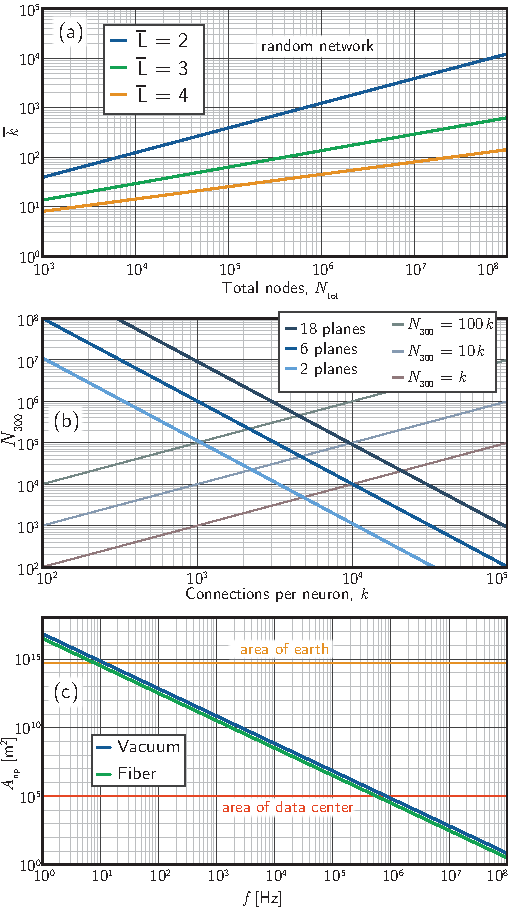
\includegraphics[width=8.6cm]{data_plots.pdf}}
	\captionof{figure}{\label{fig:data}Scaling considerations for optoelectronic neural systems. (a) The average number of connections per node required to maintain a give average path length across a random network as a function of the total number of nodes in the system. (b) The total number of nodes that can fit on a 300\,mm wafer as a function of the number of connections per node in the wire-limited regime \cite{ke1982}. (c) The area of the neuronal pool as a function of the frequency of neuronal oscillations assuming light-speed communication \cite{shICRC2018}.}
\end{figure}

\subsubsection{Clustering}
This analysis of average path length is relevant for quantifying a network's potential for information integration, but as we stated above, a neural system also depends on the ability for differentiated processing. Let us consider differentiation across various scales of the network. Ideally, no two neurons would behave identically, because this would not provide new information. Each neuron will fire preferentially in response to stimulus according to a tuning curve \cite{daab2001}. In practice, some redundancy is advantageous if a network is to rapidly gain confidence regarding the nature of a stimulus. Neural systems employ populations of neurons to represent certain pieces of information. The net activity across the population represents the presence or absence of a stimulus, and the variation in activity across the population represents uncertainty about the interpretation of the stimulus. In order for a certain population of neurons to predominantly exchange information locally and rapidly establish a consensus interpretation of a stimulus, the neurons in that population should comprise a preponderance of connections within the population. Groups of neurons with an abundance of connections within the group relative to connections external to the group form a community, and a clustering coefficient \cite{eskn2014,fa2007} is the simplest network metric. If node $a$ is connected to node $b$ and to node $c$, the clustering coefficient quantifies the fraction of cases in which node $b$ is also connected to node $c$. This metric provides insight into the tendency of neurons to form specialized communities with information processing differentiated from other parts of the network, and is first step toward analyzing the modularity of the system. 

\subsubsection{Small-World Networks}
A random network has a low clustering coefficient, as the presence or absence of a connection between nodes $b$ and $c$ is, by definition, completely independent of the presence or absence of any connections to or from node $a$. Yet the networks of the brain\textemdash from the scale of neurons to the scale of connections between regions\textemdash show a high degree of clustering relative to a random network. As we have emphasized, neural information processing relies on both differentiated processing by local clusters and efficient integration of information across the network. We therefore expect neural systems to simultaneously achieve a high clustering coefficient and short average path length. A small-world networks is one with both of these traits \cite{wast1998}. We can introduce the small-world index (SWI) \cite{hugu2008} given by  $\mathrm{SWI} = \frac{\bar{C}/\bar{L}}{\bar{C}_{\mathrm{r}}/\bar{L}_{\mathrm{r}}}$, where $\bar{C}$ is the average clustering coefficient, $\bar{L}$ is the average shortest path, and the subscript, $\mathrm{r}$, refers to a random graph. Whether analyzed at the scale of populations of a few thousand neurons or at the scale of large regions of the brain, the networks demonstrate large $\mathrm{SWI}$, indicating that different populations of neurons represent different information, the activities of these populations can be efficiently communicated across the network, and  giving hints that brain architecture is hierarchical and modular.

\subsubsection{\label{sec:modularity_and_hierarchy}Modularity and Hierarchy}
Anatomically, clusters in the brain were thoroughly described by Mountcastle in 1978 \cite{mo1978} before the concept of a small-world network had been introduced \cite{wast1998}. Mountcastle referred to the communities of neurons as mini-columns and columns. Imaging of biological neural systems with various techniques across all relevant length scales indicates modularity persists across multiple levels of hierarchy \cite{beba2017}. The clustering coefficient discussed above can be generalized to the modularity, $Q$, quantifying the degree to which the connections of a network depart from what would be expected of a random network to form partitioned communities \cite{rusp2010,beba2017}. For example, clusters of neurons are partitioned into mini-columns. At the next level of hierarchy, clusters of mini-columns are partitioned into columns. Clusters of columns are partitioned into brain regions. At the highest level of hierarchy in the brain, regions exchange information throughout the cerebral cortex and the thalamocortical complex that controls and coordinates operation of the largest modules comprising the brain. Neurons predominantly contribute to activity within their module, but they also must be able exchange information across partitions and up the information-processing hierarchy. Again we find differentiated, local processing combined with information integration across the hierarchical structure of the network. This neural information processing is enabled by a small-world architecture.

(probably need more here. make sure it is well set up for neuronal avalanches section and fractal use of space and time. define modular and hierarchical)

\subsubsection{Rentian Analysis}
%\begin{figure} 
%    \centering{\includegraphics[width=8.6cm]{rentian_analysis.pdf}}
%	\captionof{figure}{\label{fig:rentian_analysis}Caption.}
%\end{figure}
We can quantify the ability of information to be communicated up the hierarchy by analyzing the number of connections penetrating various partitions of the network, referred to as Rentian analysis. Rent's rule states that the number of edges crossing the boundary of a partition ($k$) is related to the number of nodes within the partition ($n$) by a power law of the form
\begin{equation}
\label{eq:Rent}
\varepsilon = \varepsilon_1 n^p,
\end{equation}
where $\varepsilon_1$ is the number of edges emanating from each node (first level of hierarchy), and $p$ is referred to as the Rent exponent. Rent's rule (Eq.\,\ref{eq:Rent}) was first observed in the context of VLSI circuits, and has also been shown to hold for biological neural circuits ranging from \textit{C. elegans} to the human brain \cite{bagr2010}. 

Depending on the system under study, the Rent exponent may vary, but is generally around 0.75 \cite{bagr2010}. We will demonstrate the use of Eq.\,\ref{eq:Rent} in Sec.\,\ref{sec:scaling}. The significance of the Rent exponent can be seen in its relation to the topological dimension, $D$. In Euclidean geometry, the surface area of a structure embedded in $d$-dimensional space is given by a power law of the form $s\sim v^p$. In general, the surface area $s$ scales as a length to the power of $d-1$, while the volume scales as a length to the power of $d$. Thus, in Euclidean geometry, $p = 1-1/d$, or $d = (1-p)^{-1}$. The same expression holds in fractal geometry \cite{ma1983,sc1991}, and in the case of Rentian scaling the topological dimension is related to the Rent exponent by $D = (1-p)^{-1}$, with $0 \le p \le 1$, so that $1 \le D \le \infty$. For $p > 2/3$, the topological dimension is larger than the embedding dimension, indicating that through a judicious implementation of input and output ports, information can flow through a network as if its components were connected in a higher-dimensional space. In the case of the brain, we find $D \approx 4$.

In any real network, it will only be possible to adhere to Eq.\,\ref{eq:Rent} across a certain domain of $n$. In the brain, consideration can apply from a single neuron up to the brain as a whole. Yet across this domain, Eq.\,\ref{eq:Rent} applies only piecewise, with discontinuities at certain partitions \cite{oz2004}. For example, we may expect Eq.\,\ref{eq:Rent} to hold from the scale of a single neuron up to the scale of a cortical column, but the connectivity patterns between columns are quite different than within, so we may expect a discontinuity at the scale of cortical columns, followed by a new expression of Eq.\,\ref{eq:Rent} with a different value of $p$, and perhaps a new interpretation of $n$ as the number of columns within a partition. Similarly in the domain of microelectronics, a multicore processor on a chip may obey Eq.\,\ref{eq:Rent} within each processor, with a discontinuity at the scale of the connections between processors. The wiring organization of VLSI circuits and the brain is statistically fractal, but not infinitely so. The limitations are purely physical.  

How does Rentian analysis inform our design of neural hardware? As we have emphasized, neural information is processed across a modular hierarchy. Rentian analysis quantifies the ability of information to be transmitted across partitions in the hierarchy. We conjecture that the ability for a neural system transmit more information across more levels of hierarchy will improve general intelligence. Therefore, between the neurons within a module, we expect that neural hardware should achieve high values of $D$ over a large range of $n$ before a discontinuity is necessary, so that multiple levels of hierarchy can be traversed efficiently within a module. Further, upon encountering a discontinuity, hardware must have a means of establishing another domain of Rentian scaling to efficiently collect and distribute information across more orders of hierarchy. Finally, we conjecture that the most intelligent neural hardware will provide this fractal scaling across as many levels of hierarchy as possible until the system finally reaches the limits set by the speed of communication. In Sec.\,\ref{sec:scaling} we will discuss these large-scale limits in biological and optical systems.

\subsubsection{Summary of Spatial Considerations}
The spatial structure of a neural system must comprise nodes with many edges to enable short path length across large networks. These nodes must also have high clustering to enable differentiated processing within modules. The information from these modules must be integrated across the hierarchy of the network, and the ability to do so is quantified by the topological dimension. Neural systems efficiently process information through the fractal use of space. Let us now consider their operation in time.

\subsection{Temporal Dynamics of Neural Systems}
We emphasize that neural systems make use of space and time in a coordinated manner. We have described the spatial properties of neural systems in the preceding subsection, and here we describe the temporal dynamics. In the following subsection we describe how neural systems process information across space and time to enable cognition. 

Due to the complexity of neural information processing, multiple different perspectives have emerged that emphasize different aspects of observed phenomena. These perspectives are not necessarily mutually exclusive, and a complete understanding of neural systems may require all of these concepts. This situation is analogous to the parable of the blind men and the elephant, in which several individuals attempt to understand the full nature of an elephant with access to only a subset of the relevant physical data. This analogy leads us to identify the neural elephant, depicted in Fig.\,\ref{fig:neural_elephant}. This analogy illustrates that the challenge of understanding neural information processing at the scale of the human brain is challenging enough that multiple perspectives are required to grapple with the phenomena observed to date. Here I discuss three primary perspectives that have been brought to bear on the problem. These three perspectives are: 1) oscillations and synchrony; 2) the mathematical framework of dynamical systems; and 3) neuronal avalanches and criticality. All three of these perspectives emphasize the interplay between space and time, and in Sec.\,\ref{sec:cognition} we will argue that they are all related phenomena, but like different parts of the same neural elephant.
%\begin{figure} 
%    \centering{
\includegraphics[width=8.6cm]{neural_elephant.pdf}}
%	\captionof{figure}{\label{fig:neural_elephant}Caption.}
%By Hanabusa Itchō - This is a retouched picture, which means that it has been digitally altered from its original version. Modifications: rotated, cleaned, cropped, centerline fold/crease removed (original Ukiyo-e print was on two pages), and scan fog haze removed., Public Domain, https://commons.wikimedia.org/w/index.php?curid=2265247
%\end{figure}

Before exploring these three perspectives on dynamical activity in neural systems, it is necessary to review basic behaviors at the device level. In the next subsection we describe neuronal device dynamics, including relaxation oscillations, neuronal communication mechanisms, synaptic plasticity mechanisms, and computations performed by synapses and dendrites. 

\subsubsection{Device Dynamics}
A neuron is a dynamical entity. It receives input from many afferent synapses, identifies coincidences and sequences between the activities on multiple synapses, and integrates various inputs over time. In a biological neuron, activity on a synapse results in a post-synaptic current into the receiving neuron. This current reduces the magnitude of the voltage across the neuron's cell membrane, usually with an exponential decay in time, and if that voltage is reduced below a threshold, the neuron produces an action potential, often referred to as a spike or pulse. This dynamical process of signal accumulation followed by bursting activity qualifies a neuron to be considered a relaxation oscillator. Before describing the temporal dynamics of neural systems in more detail, let us consider for a moment why relaxation oscillators are particularly well suited for cognition.

\paragraph{Relaxation Oscillators}
As we have mentioned, a defining aspect of cognitive systems is the ability to differentiate locally to create many sub-processors, but also to integrate the information from many small regions into a cohesive system, and to repeat this architecture across scales. A network of many dynamical nodes, each with the capability of operating at many frequencies, gives rise to a vast state space. As computational primitives that can enable such a dynamical system, oscillators are ideal candidates. In particular, relaxation oscillators \cite{st2015,mist1990,soko1993,lued1997,huya2000,bu2006,gile2011,vepe1968,cacl1981} with temporal dynamics on multiple time scales \cite{soko1993} have many attractive properties for neural computing, which is likely why the brain is constructed of such devices \cite{ll1988}. We define a relaxation oscillator as an element, circuit, or system that produces rapid surges of a physical quantity or signal as the result of a cycle of accumulation and discharge. Relaxation oscillators are energy efficient in that they generally experience a long quiescent period followed by a short burst of activity. Timing between these short pulses can be precisely defined and detected \cite{bu2006}. Relaxation oscillators can operate at many frequencies \cite{huya2000,more} and engage with myriad dynamical interactions \cite{lued1997}. The oscillator's response is tunable \cite{huya2000}, they are resilient to noise because their signals are effectively digital \cite{stgo2005}, and they can encode information in their mean oscillation frequency as well as in higher-order timing correlations \cite{pasc1999,thde2001,sase2001,stse2007,brcl2010,haah2015}.

\paragraph{Information Coding by Relaxation Oscillators}
The spiking nature of relaxation oscillators enables them to encode information in several ways. Most simply, they can encode information in their average firing rate, which gives rise to the standard expression used in deep learning and neural networks:
\begin{equation}
\label{eq:standard_neural_network_activation} 
y_i = f(\sum_{ij}w_{ij}y_j),
\end{equation}
where $y_i$ represents the ``activation'' of the $i$th neuron, $w_{ij}$ is the synaptic weight from neuron $j$ to neuron $i$, and $f(\cdot)$ is a nonlinear function representing the input-rate-to-output-rate transfer function of a simple point neuron. Equation \ref{eq:standard_neural_network_activation} is an extremely simple model of a neuron in the sense that only the average firing rate is considered, so no information regarding the precise times of spikes is retained. Further, $w_{ij}$ is assumed to be independent of frequency, so the model assumes synapses and dendrites perform no spectral filtering. Also, all input synapses are assumed to terminate on a single integrating body, assumed to be the soma, so no information regarding the spatial location of the synapse on the dendritic tree is retained. Nevertheless, Eq.\,\ref{eq:standard_neural_network_activation} has proven remarkably useful as a starting point for deep learning. 

Beyond the rate-coded, point neuron model, relaxation oscillators can also encode information through several other means. These include the time-to-first-spike after the onset of a stimulus, the phase of a spike relative to sinusoidal background oscillations, and the time interval between the firings of two or more neurons (see Sec. 4.5 in Ref.\,\cite{geki2002}). Thus, while information coding in digital computing is simple (bits are transmitted one at a time on a clock), information processing in neural systems with relaxation oscillators as computational primitives is complex. Neurons and networks do not speak a single, simple language, but rather send various types of spike-based messages with different information encoding and decoding in different contexts. We will explore these various strategies for coding in more detail shortly, but first we note one simplifying factor: the spikes that are used to communicate between neurons are binary. No information is conveyed in the amplitude of a single spike.

\paragraph{Binary communication and post-synaptic response}
We expect that any cognitive computing platform will be based on spiking neurons that behave as relaxation oscillators. Communication between these relaxation oscillators is effectively binary\textemdash all or nothing. When a neuron produces an action potential, it propagates down the axon and branches throughout the axonal arbor. The signal propagates as a section of depolarization between the interior of the axon and the surrounding extracellular fluid. This depolarization opens pores in the membrane of the axon, allowing the flow of ions from the extracellular fluid into the axon, thus providing the electrical signal that will reach the synapses. Each time the action potential is generated, the behavior is nearly identical: the speed of propagation of the signal is set by the physical properties of the axon; the number of pores that open is very large, so the signal propagating down the axon is not noisy; and the signal that reaches the synapses is very similar from pulse to pulse. Significant variability arises when an action potential meets a synapse, but this relates to the information processing occurring at the synapse (discussed in more detail below), not the nature of the encoding of the signal. 

To realize the digital nature of neuronal communication, the role of the action potential propagating down the axon is not to provide current to the post-synaptic neuron, but rather to begin a chemical cascade within the synapse that controls the post-synaptic signal amplitude. When the action potential reaches the synapse (pre-synaptic cleft), the action potential may trigger the release of neurotransmitters into the synaptic cleft. These neurotransmitters diffuse through the fluid of the cleft, and bind to receptors on the post-synaptic cleft. These receptors then trigger the flow of current through the dendrite on which the synapse resides. This post-synaptic current carries the information that will be processed, first by the dendrite, then the dendritic tree, and finally the soma. The action potential arriving at the synapse initiates the synaptic cascade in a binary, all-or-nothing manner (either vesicles are released from the pre-synaptic cleft or they are not), but the amount of current flowing into the post-synaptic dendrite depends on the state of the synapse, and it can take a continuum of values. Thus, communication in neural systems is binary, yet information processing is analog. The synapse performs a digital-to-analog conversion, and the state of the synapse (which depends on many factors) determines the analog value entering into the computation performed by the dendrites and soma. 

When a synapse receives an action potential, it has a certain probability of releasing vesicles containing neurotransmitters that will then be detected on the receptors of the post-synaptic cleft, generating a current that will propagate a certain distance and decay with a certain time constant. The time-course of the response is a continuous function, specifically an exponential decaying in space and time. The length and time constants depend on: the type of synapse; the morphology of the dendrite to which it is connected; the concentration of various neuromodulators; and the local membrane potential, which is determined by local synaptic activity. Thus, communication between neurons is well modeled by binary events that trigger a post-synaptic current with some probability $P_{\mathrm{s}}$, while the post-synaptic current is highly variable and shaped by a number of physiological and dynamical factors. We will further explore the relevance of this post-synaptic response in the coming paragraphs. 

\paragraph{The Neuron as a Complex Information Processing System}
For multiple reasons described above, we expect relaxation oscillators to be the computational primitives of complex cognitive systems. But amongst relaxation oscillators, neurons are unique in the myriad complexities. Our understanding of the information-processing capabilities of neurons has evolved considerably over time. Early models treated a neuron as a point that passively integrated many inputs and produced a signal upon reaching threshold. This integrate-and-fire model was proposed as early as 1906 by Sherrington in a series of lectures \cite{sh1906}, supporting the view championed by Ram\'{o}n y Cajal \cite{ra1908}. It was that same year that Ram\'{o}n y Cajal shared the Nobel Prize in Physiology or Medicine with Golgi for their work on the structure of the nervous system. Within this point-neuron view, a neuron simply integrates signals over time, so information regarding the timing or location of synaptic activity is lost. Further, the complex, dendritic tree is assumed to passively transmit synaptic signals to the neuron cell body. 

This view of the neuron as a point integrator was highly influential, and remains the dominant model guiding many efforts in deep learning and even neuromorphic hardware. However, further experimental evidence as well as theoretical arguments have deepened our understanding of how neurons work and led to a picture of neural information processing that is far more subtle and powerful. 

The modern picture of neural information processing reveals that many operations in addition to integration are being performed, and that these computations are performed at synapses, through the dendritic tree, and in the neuron as a whole. Some of the additional operations now believed to be performed by neurons include: coincidence and sequence detection; nonlinear thresholding performed in dendrites; temporal filtering of pulse trains; and bursting to overcome noise and enable selective communication between subsets of neurons in an ensemble. We now review each of these concepts and explain their significance for neural information processing.

\paragraph{Coincidence and Sequence Detection in Active Dendrites}
As discussed above, after a synapse is triggered and a post-synaptic response is induced, the time-course of the post-synaptic response is a decaying exponential with a time constant that can be shaped by a number of factors. Whether a neuron simply integrates signals or detects coincidences depends on this time constant of the post-synaptic potential relative to the average neuronal interspike interval. If the time constant is on the order of the interspike interval of the neuron, temporal integration is performed during the entire interspike interval, and the neuron is well-modeled as an integrator. If the time constant is short compared to the interspike interval, neurons perform coincidence detection, meaning only spikes that are coincident on the neuron within a short time window relative to the interspike interval can induce the neuron to produce an action potential. If integration is performed exclusively, then the timing of spikes conveys no information. If coincidence detection occurs, information is conveyed in spike timing, neurons respond preferentially to synchronized inputs, and a neuron's output reflects the input pattern.

Work in the 1990s led K\"{o}nig, Engel, and Singer to argue that cortical neurons are better modeled as coincidence detectors than integrators \cite{koen1996}. Their arguments were based both on the physiological evidence that many synapses can have time constants much shorter than the average interspike interval as well as theoretical arguments related to information processing. Regarding the latter, multiple benefits can be identified. First, speed of response can be improved if coincidences can be utilized. Processing speed is determined by the latency between the time of arrival of a signal and the time of a generated response. As stated in Ref.\,\onlinecite{koen1996}, ``Because only a small subset of all afferent [post-synaptic potentials] are relevant (namely those which actually conicide and trigger an action potential), the mean time-lag between relevant input and output signals is very short\textemdash only a fraction of the interspike interval. Thus, at identical interspike intervals neuronal systems utilizing coincidence detection can process information much faster.'' Second, coincidence detection provides benefits with regard to error propagation and noise. Errors due to stochastic processes in the environment are effectively filtered out by coincidence detection, as they would only contribute to neuronal firing rarely when they coincide with true signal, whereas neurons performing integration sum all incoming activity uniformly, regardless of correlations that may serve to isolate signal from noise. Third, the use of coincidence detection allows neural systems to make use of smaller ensembles of neurons for encoding information, referred to as the size of the `grain' in Ref.\,\onlinecite{koen1996}. If coincidences give rise to larger post-synaptic signals, then synchronized activity of a small group of neurons can have a large effect and drive a neuron to spike. Finally, the main strength of coincidence detection temporal information is not discarded, and synchronized inputs are processed differently than asynchronized inputs on the same set of synapses. The ability to respond preferentially to synchronized inputs has important consequences for information integration and binding, as discussed below in Sec.\,\ref{sec:oscillations_and_synchrony}. If neurons can detect coincidences, several important computation become possible. 

Work elucidating the behavior of dendrites further supports the view that neurons make use of the timing of synaptic activity as well as other intricacies beyond simple integration \cite{stsp2015}. As stated by Koch in 1997, ``...dendrites do much more than simply convey synaptic inputs to the cell for linear summation. Indeed, if this were all they did, it is not obvious why dendrites would be needed at all; neurons could be spherical in shape and large enough to accommodate all the synaptic inputs directly onto their cell bodies. ...the function of this elaborate structure cannot simply be to maximize the surface area for synaptic contact.'' \cite{ko1997} Instead of acting as passive transmission lines, the active properties of dendrites \cite{joma1996} give rise to the ability to detect coincidences. The basic mechanism relies on the nonlinearity of the response of a dendrite. If two synapses are located in close proximity on a dendrite, the response of the dendrite is a nonlinear function of the activities of the two synapses. Whereas the response of a passive dendrite would be the sum of the activities of the two synapses, the true dendritic response is closer to the product of the activities of the two synapses \cite{ko1997}. Further, dendrites themselves can generate spikes upon reaching threshold \cite{hoko2006}, a behavior once thought only to occur in the neuron as a whole. Again considering the example of two synapses on a dendrite, if only one of the synapses fires within the decay time of the post-synaptic potential, it may be insufficient to generate a dendritic spike, and the neuron is not informed of the synaptic activity. However, if both synapses fire within the decay time it may be sufficient to induce a dendritic spike, and the information is passed along the dendritic tree toward the soma. By 2006, the physiological mechanisms of dendritic spikes were more clearly understood \cite{hoko2006}, providing the device-level mechanism to support the coincidence-based information processing described by K\"{o}nig, Engel, and Singer in 1996. The nonlinear response of a dendrite with two synapses can also be compared to a logical AND operation: if synapse one AND synapse two fire within a certain time window, an output pulse is produced. 

The processing capabilities of dendrites extend beyond detection of coincidences between two synapses. Consider now $n$ synapses connected to a single dendrite. Now the dendrite will perform a nonlinear function on the inputs of the $n$ synapses, leading to an intermediate nonlinear transfer function between the synapses and the neuron as a whole. A neuron comprising many such dendrites will behave as a complex processor comprising multiple independent threshold units, and giving rise to myriad different transfer functions depending upon precisely which afferent synapses are active at a given time, just as observed in recent experiments \cite{sava2017}. Further, due to the morphology of a given dendrite, the post-synaptic current will often flow in a particular direction, usually toward the cell body. Consider the case where synapse one makes contact furthest from the cell body and synapse $n$ makes contact closest to the cell body. In this case, firing of synapse one will lead to a post-synaptic current that flows toward synapse two, thereby lowering the local membrane potential at synapse two. If a synaptic firing event at synapse one is followed closely by a firing event at synapse two, dendritic current is more likely to propagate on to synapse three, thereby lowering the membrane potential there. The pattern extend to synapse $n$, and this nonlinear signal propagation along the dendrite provides a means for the dendrite to detect specific sequences of activity: if synapse one fires just before synapse two, and synapse two is just before three, etc., then the dendrite is far more likely to produce a spike that propagates to the cell body than if the synapses fired in a different order. This phenomenon is illustrated schematically in Fig.\,\ref{fig:dendritic_sequence_detection}. The ability of neurons to make use of such sequence detection was developed in 2016 by Hawkins and Ahmad \cite{haah2015}. (say a bit more here) Interestingly, humans appear to be the species with the most elaborate dendritic trees \cite{el2003}.

\vspace{3em}
The total potential generated along a dendrite ``depends therefore on the temporal order of the stimulation of the synapses. An input sequence starting at the far end of the dendrite and approaching the soma is more effective in triggering an output spike than the same number of input spikes in reverse order.'' (\cite{geki2002}, pg. 144.)

%\begin{figure} 
%    \centering{\includegraphics[width=8.6cm]{dendritic_sequence_detection.pdf}}
%	\captionof{figure}{\label{fig:dendritic_sequence_detection}Caption.}
%\end{figure}

I will discuss dendrites further in the context of learning and plasticity shortly. First I review work related to communication between neurons through bursting.

\vspace{3em}
For detection of temporal information in the brain, cite review article from 1993 \cite{ca1993}. You have not read this article, so be careful.

\paragraph{Communication in Bursts}
If neurons encoded information only in their average firing rate, we would expect most neurons to fire relatively consistently, with the exact value of the rate dynamically varying depending on stimulus. By contrast, if neurons encoded information only in spike timing and coincidences, we would expect them to fire single action potentials when presented with relevant stimuli. In practice, these two behaviors are both observed, but a more common mode of activity is the burst. A neuronal burst is a closely spaced sequence of spikes followed by a long quiescent period. 

%bursting for reliability
Bursting activity is thought to play a central role in communication between neurons, perhaps as important as rate or other forms of temporal coding. One function of communication via bursts was appreciated by the 1990s, and that is the increased reliability of communicating with bursts rather than single spikes \cite{li1997}. A single synapse can be unreliable at producing a post-synaptic current in response to the arrival of a single action potential. On the device level, this is because vesicle release by the pre-synaptic cleft does not occur deterministically, but rather with probability $P_{\mathrm{s}}$, which varies considerably across synapses, and can be less than 0.1. However, the arrival of a number of action potentials in close succession performs a facilitating function that increases the probability of vesicle release with the arrival of each successive pulse. While the synaptic response to a single action potential can be unreliable, the response to a burst is much more reliable, increasing $P_{\mathrm{s}}$ above 0.9 simply by using two pulses instead of one in some observations \cite{fomc1991,degu1996}, a phenomenon known as paired-pulse facilitation \cite{li1997}. 

This reasoning of bursts being more reliable than single spikes is intuitive, but it may lead one to suspect that bursts effectively make communication analog in the sense that the generated post-synaptic current will depend on the number of spikes in the burst. Lisman has argued based on physiological evidence that this is not the case. The nuances of vesicle release and neurotransmitter detection are such that the post-synaptic current is nearly identical when receiving a burst, independent of the number of spikes in the burst (within a workable range) \cite{li1997}, thereby enabling bursting to overcome synaptic failure while maintaining binary communication.

Within this picture of neuronal bursting, the low probability of synaptic response becomes advantageous for filtering noise. As Lisman argues, in some brain regions, single spikes are simply the result of noise, but bursts are rarely noise. Therefore, if a synapse responds only to bursts of two or more pulses, it effectively ignores the noise, and responds only to the signal. For example, place cells in the hippocampus \cite{frbu2018} fire preferentially when the organism is in a specific location for which that neuron's tuning curve is maximized. It has been shown that responding only to bursts can define the place field more accurately than when single spikes are considered \cite{otei1991}. Similarly in visual cortex, it is well-known that neurons can have a tuning curve maximized to detect gratings with a specific spatial frequency or orientation \cite{daab2001}. It has been shown that only the bursting component of a neuron's activity is tuned to represent these quantities, while isolated spiking activity only correlates with the contrast of the light and dark regions of the grating \cite{cama1981}. These ideas lead Lisman to conclude ``that the ability of synapses to not transmit single spikes might be a crucial form of filtering.'' \cite{li1997} 

%bursting for frequency-selective communication
The concept that neurons fire in bursts to overcome unreliable synapses and filter noise is well supported by theoretical and experimental evidence. Yet these may not be the only reasons for communication in bursts. Izhikevich et al. have argued another principle is also in play: ``bursts with specific resonant interspike frequencies are more likely to cause a postsynaptic cell to fire than are bursts with higher or lower frequencies. '' \cite{izde2003} Within this model, neurons firing in bursts are like radio transmitters, and some synapses are tuned to receive spike trains of the same frequency. This tuning of synaptic and neuronal responses can be achieved through a combination of high- and low-pass filtering as well as subthreshold oscillations of the membrane potential. These device mechanisms for frequency selectivity are discussed below in Secs.\,\ref{sec:short_term_plasticity} and \ref{sec:subthreshold_membrane_oscillations}. 

The most exciting aspect of this use of bursting is that ``the same burst could resonate for some synapses or cells and not resonate for others,'' thereby providing ``effective mechanisms for selective communication between neurons.'' Such a method of targeted communication is one of many examples of how neurons can utilize one vast structural network to enable myriad functional networks at different times in different contexts. Izhikevich et al. argue that communication via bursts enables targeted, resonant communication \textit{in addition} to making communication more reliable and filtering noise. In addition to these motivations related to improvements in communication, bursts may also be more effective at modifying synaptic efficacy. I discuss the role of bursting in long-term synaptic modification below in Sec.\,\ref{sec:long_term_plasticity}.

\paragraph{\label{sec:coding_strategies_summary}Summary of Coding Strategies}
We have discussed rate coding, coincidence detection, sequence detection, and bursting. One may ask the question, ``Which of these is actually used by the brain?'' The answer is all of them. In some contexts, the average firing rate of a neuron may represent the content of a stimulus. In other contexts, the precise timing between two synaptic events or the order in which multiple synapse events occurs carries information that is utilized by the receiving neuron. In still other contexts, bursts are used to increase reliability, filter noise, and the frequency of pulses within a burst can enable selective communication between resonant elements of the network. All of these coding strategies and communication mechanisms contribute to the extraordinary efficiency and adaptability of biological neural systems, and we should aspire to incorporate all of these principles in the design of hardware for general intelligence. 

We now summarize the mechanisms at the device level that enable these subtle and sophisticated mechanisms for information processing.

\paragraph{\label{sec:short_term_plasticity}Short-Term Synaptic Plasticity}
As described above, the ability of a synapse to respond preferentially to activity at a specific frequency enables additional complexities in communication. At the device level, frequency-selective synaptic response is enabled by filtering mechanisms referred to as short-term synaptic plasticity. 
%Fig. 1 of \cite{izde2003}
%\begin{figure} 
%    \centering{\includegraphics[width=8.6cm]{short-term_plasticity.pdf}}
%	\captionof{figure}{\label{fig:short-term_plasticity}Caption.}
%\end{figure}
The state of a synapse is affected by its activity over short and long time scales as well as external network factors. Neurons often signal in bursts (closely spaced sequences of spikes) \cite{iz2007}, and within a burst, the time between spikes is referred to as the inter-spike interval. Changes of synaptic response over time scales on the order of the inter-spike interval are referred to as short-term synaptic plasticity \cite{abre2004}. One key effect of short-term plasticity is to perform a temporal filter on an afferent spike train. This can be a high-pass, low-pass, or band-pass filter, as shown in Fig.\,\ref{fig:short-term_plasticity}. High-pass filtering results in only the first few pulses of a train being transmitted from the pre-synaptic axon to the post-synaptic dendrite. A synapse performing high-pass filtering reports to the post-synaptic neuron that the pre-synaptic neuron has begun to fire. Conversely, low-pass filtering results in synaptic response after the first several pulses of a train have occurred. A synapse performing low-pass filtering will not be active unless the pre-synaptic neuron produces a pulse train of a certain minimum duration, and therefore this synapse reports to the post-synaptic neuron when the pre-synaptic neuron has sustained bursting activity beyond a certain duration. Band-pass filtering combines these responses. A synapse performing band-pass filtering will only produce a response after an afferent pulse train exceeds a certain duration, and it will fall silent again after if the afferent pulse train continues beyond a certain duration.

These short-term filtering mechanisms enable synapses to report much more information to the neuron than simply the time-averaged rate of afferent activity. A neuron combining the signals from many synapses with various short-term responses has access to information regarding not just the average spike rates of the neurons from which it receives synaptic connections, but also regarding the initialization of bursting and the duration of spike trains.


\paragraph{\label{sec:subthreshold_membrane_oscillations}Subthreshold Membrane Oscillations}

\paragraph{\label{sec:long_term_plasticity}Long-Term Synaptic Plasticity}
%\begin{figure} 
%    \centering{\includegraphics[width=8.6cm]{stdp.pdf}}
%	\captionof{figure}{\label{fig:stdp}Caption.}
%\end{figure}
Over time periods much longer than the inter-spike interval, the response of synapses can also change based on the activity of the two neurons involved in the synapse. A synapse that is more active will strengthen (long-term potentiation), and a synapse that is used less will weaken (long-term depression). This was the essential insight of Hebb in 1949 \cite{he1949}, a concept that developed in the subsequent decades \cite{bipo1998,somi2000} to account for the fact that long-term potentiation only occurs if the pre-synaptic neuron fires just before the post-synaptic neuron, indicating the potential for causality, while long-term depression is induced when the pre-synaptic neuron fires just after the post-synaptic neuron. This spike-timing-dependent plasticity (STDP) \cite{mage2012} plays a central role in memory formation and network adaptation. 

The physical mechanism responsible for STDP involves the growth and decay of neurotransmitter sources and receptors present at the synapse. These synaptic molecular machines (N-methyl-D-aspartate receptors, NMDARs) develop in response to the action potential arriving at the pre-synaptic terminal as well as the back-propagating signal from the post-synaptic neuron. The complex chemistry present at each synapse leads to a remarkable degree of diversity and adaptability in synaptic response.

By strengthening cooperative synapses, STDP adapts the structural network of neurons and their connections into functional networks embodying certain memories or computations learned over time based on the correlations of neuronal firing events. It has been shown that random networks with synaptic weights adjusted over time by STDP adapt into small-world networks \cite{shki2006}, maintaining efficient communication, and adding functional clusters specialized for specific computations. This is one example of the structural network of a neural system can be used to manifest multiple functional networks.

The functional clusters established via STDP have spectral signatures. A given functional cluster of neurons will have a specific pattern of activity, that may repeat in time. The period of this repetition will depend on the specific parameters of the circuit, and a large structural network comprising many highly connected neurons will have the potential to establish a vast repertoire of functional clusters with oscillations at many frequencies. Through STDP, the network can increase the activity of certain oscillations corresponding to highly utilized functional modules. If a certain stimulus has a probability of activating a certain functional cluster, the overtime, the action of STDP will enable the network to correlate that stimulus with the dynamical response of the cluster, and the stimulus will evoke the activity of the cluster with higher probability. In the language of dynamical systems, a specific cyclical response of the functional cluster is referred to as a basin of attraction \cite{iz2007,st2015}, and STDP ensures that relevant stimuli lead the network to the appropriate basin of attraction. This is function of an autoassociator, and it is an important form of long-term memory (\cite{bu2006} pg. 329).

Spike-timing-dependent plasticity makes use of correlations between firing activity of neurons to adapt the network into functional clusters \cite{shki2006}, store memories in dynamical sequences \cite{haah2015}, and strengthen circuits that demonstrate temporal patterns storing sequential memories (\cite{bu2006} pg. 318). But theoretical analysis finds that if STDP is the only long-term synaptic plasticity mechanism, memories are forgotten very quickly \cite{fuab2007}. Experimental analysis finds that synapses have multiple additional means to change how synapses adapt over time and activity to help retain memories \cite{ab2008}. These plasticity mechanisms are referred to collectively as metaplasticity.

%bursting for plasticity
It has been shown that a burst of action potentials comprising four pulses can be sufficient to induce long-term potentiation and depression \cite{huli1995}, dependent on the timing of the burst relative to theta oscillations. A burst arriving at the peak of theta leads to potentiation, while a burst arriving at the trough leads to depression. In this case, we find an interplay between neuronal bursting, synchronized oscillations, and synaptic plasticity. Adapting based on the confluence of all this information leads to efficient evolution toward a network structure that generates constructive activity.

\paragraph{Metaplasticity}
While STDP adapts the strength of synapses (synaptic efficacy), metaplasticity adapts the rate at which synaptic efficacy changes over time and activity. For example, if a pre-synaptic neuron fires just before a post-synaptic neuron, the synapse connecting the two will be a candidate to experience long-term potentiation. But the \textit{probability} that the synapse actually does potentiate can be controlled by chemical signals within the synapse. Additionally, the \textit{amount} by which the synaptic efficacy changes is also subject to chemical modulation. 

The function of metaplasticity is to control which neural circuits adapt at a given time \cite{ab2008}. The receptors mentioned above (NMDARs) can be controlled based on a variety of factors related to network activity so that adaptability may be turned on and off in certain regions at certain times. This functionality is required of plastic synapses to keep them from too quickly losing the trace of a memory that is still needed. Experiments with humans indicate that forgetting occurs as a power-law function of time, \cite{wieb1991,wieb1997}, yet Fusi and Abbott have shown that memories are lost more rapidly than this if plastic synapses are presented with continual stimulus \cite{fuab2007}. They have proposed a model that achieves the observed power-law forgetting by introducing internal complexity to the synapses \cite{fudr2005}. In this model, each synapse has various states of efficacy (weak and strong synaptic weight), but it also has additional internal states with the same efficacy. The difference between these states is the probability with which the efficacy will change due to future plasticity events. 

Metaplasticity provides a network with the means to to enable some regions to adapt at a given time, under a given stimulus, while other regions are unchanged at that time, under that stimulus. Further, metaplasticity provides a means by which some synapses within a region may change very rapidly to adapt to a new stimulus, while other synapses in the same region may change slowly or not at all when presented with the same stimulus. We expect that an intelligent neural system have the capability to immediately learn in response to new information, but also to maintain a lasting representation of all that has been learned through the network's existence even in the presence of continually varying input. Metaplasticity is an important means by which rapid learning in conjunction with long memory retention can be achieved. As stated by Abraham, ``...these metaplasticity processes represent a major form of adaptation that helps to keep synaptic efficacy within a dynamic range and larger neural networks in the appropriate state for learning.''

\paragraph{Homeostatic Plasticity}
To conclude this discussion of synaptic plasticity mechanisms, we note that short-term plasticity adapts based only on the activity of the pre-synaptic neuron, while STDP adapts based on correlations in the activity between pre- and post-synaptic neurons. The mechanism of homeostatic plasticity \cite{cube2012} adapts synaptic weights based only on the activity of the post-synaptic neuron. Homeostatic plasticity (also referred to as the Bienenstock-Cooper-Munro (BCM) model \cite{bico1982}) adjusts the synaptic weights of synapses incident upon a given neuron based on a sliding temporal average of the recent firing activity of that neuron. Such a mechanism provides a means by which neuron and network activity can be maintained within useful limits and dynamic range can be maximized.

\paragraph{\label{sec:dendritic_processing}Dendritic Processing}
We have discussed how STDP leads to the formation of functional clusters within a network based on the history of correlated neuronal activity. But what if the network wishes to isolate specific functional clusters on time scales as short as an inter-spike interval? Or what if we wish to endow a neuron with the ability to respond not only to activity in single synapses, but rather to integrated activity from specific clusters of synapses, or to specific sequences of activity within a cluster of synapses? Dendritic processing enables these functions.

Dendritic processing refers to the intermediate, nonlinear transfer functions performed by dendrites between individual synapses and the neuron as a whole \cite{stsp2015}. The dendritic arbor is a complex, branching structure on which most of a neurons input synapses make their connections. While the dendritic tree was thought to be a passive integrating structure for quite some time, by the mid 1990s many activite dendritic responses were beginning to be understood \cite{joma1996}. The dendritic branches that comprise the arbor have passive and active properties that allow them to perform various computations. Dendrites modulate postsynaptic potentials on their way to the soma as well as generate spike activity \cite{majo2005,hoko2006}. One picture of the dendritic arbor is a network of multiple independent threshold units that integrate signals and produce dendritic spikes upon reaching threshold. This picture was introduced on theoretical grounds based on the enhanced storage capacity of such a dendritic tree in 2001 \cite{pome2001}, and supporting experimental evidence continues to accure \cite{sava2017}.

For example, consider a dendrite with two synapses. If the post-synaptic current into the dendrite is sufficient to produce a dendritic spike, and if this dendritic spike has the same form whether one or both synapses fire, the dendrite performs the OR operation. If both synapses are required to fire to produce a dendritic spike, it performs the AND operation. The current generated in a dendritic spike propagates only a short distance along the dendritic tree, into the next dendritic compartment closer to the cell body, and the current decays with an exponential time constant. Thus, dendrites can perform basic logical operations with a temporal component, and activity closer to the base of the dendritic tree at the cell body integrates information from a larger number of inputs. 

Like many aspects of neural information processing, the myriad roles of dendrites remind us that the devices giving rise to cognition are diverse and multifunctional. Mel, Schiller, and Poirazi emphasize that ``dendrites of different neuron types contribute to the cell's input-output function in markedly different ways.'' \cite{mesc2017} While all of the aforementioned roles of dendrites are observed in biological neural systems, they are not necessarily all present in every dendrite. In the context of designing hardware for neural information processing, these functions must be available, and sophisticated analysis at the level of networks and systems must inform our decisions of when to include each mechanism.

\cite{pome2001}

\paragraph{\label{sec:dendrites_and_plasticity}Dendrites and Plasticity}
In addition to performing nonlinear transfer functions on inputs, dendrites also play a key role in synaptic update and learning. This activity is induced by back-propagating action potentials created during the firing of the neuron \cite{majo2005}. These back-propagating action potentials provide a feedback signal from the neuron to the dendrites and synapses after neuronal firing that performs one of the steps in a timing-dependent plasticity process \cite{nesa2004}.

In addition to back-propagating action potentials playing a role in STDP, dendritic spikes are also involved in forms of synaptic plasticity that do not require synaptic activity. In these forms of synaptic plasticity, it is the timing of the forward-propagating dendritic spikes and backward-propagating spikes that establish the conditions in which synaptic weights can be modified \cite{hoko2004}. This local activity can lead to long-term synaptic potentiation or depression and may be the primary mechanism for rapidly acquiring memories \cite{hoko2006}.

We have mentioned that dendrites are capable of acting as integrators or coincidence detectors depending on the time constants involved. Additionally, a single dendrite can transition between these two roles based on the interplay between synaptic activity and the neuromodulatory environment \cite{hoko2006}. The presence of certain neuromodulators affects the behavior of voltage-gated ion channels, thereby shaping the short-term response of dendrites \cite{majo2005}. As stated by Holthoff et al., ``...the alliance of non-linear and linear integration modes combines the advantages of the excellent signal-to-noise ratio of digital processing with teh speed and complexity of analog processing.'' \cite{hoko2006} 

We have also mentioned that back-propagating action potentials in dendrites play a central role in STDP. The active properties of dendrites can lead to metaplasticity as well \cite{ab2008}. The mechanisms involved again relate to the interactions between synaptic inputs and neuromodulators. The interplay between neuromodulators and synaptic activity affects the time constants that shape the dendritic membrane potential as well as the probability that potentiation or depression will occur in the presence of synaptic input. 

This discussion of dendritic processing is necessarily brief, emphasizing the active role played by dendrites in adaptive and frequency-selective response to spike trains based on voltage-dependent conductances; the nonlinear thresholding properties of dendrites exemplified by the generation of dendritic spikes; and the role of the dendritic tree and back-propagating action potentials in synaptic plasticity. Further detail can be found in the comprehensive review by Sj\"{o}str\"{o}m et al. \cite{sjra2008}

\paragraph{Summary of Neural Device Dynamics}
This subsection summarized literature supporting the perspective that relaxation oscillators are uniquely suited to serve as computational primitives in cognitive systems due to the high signal-to-noise ratio of their outputs, their adaptive frequency response, and their ability to make use of many information coding schemes. These coding schemes have been described. The importance of binary communication for mitigating noise was discussed, and multiple communication schemes were explained. These modes of communication include: average rate; coincidence and sequence; phase relative to background oscillations; and bursting for reliability as well as frequency selectivity. The device-level mechanisms that enable these functions were summarized, including short- and long-term synaptic plasticity and active dendritic functions. We now turn our attention to activity emerging from populations of neurons.

\subsubsection{\label{sec:populations}From devices to populations}
We have described some of the basic device operations of neurons and their components, but neural information processing leverages entire populations of neurons with emergent mechanisms for information processing occurring in a network context. As a first example, consider a population of uncorrelated, non-interacting neurons receiving identical stimulus and firing asynchronously. The population activity is defined as the sum over all firings by all neurons, and in the presence of a constant stimulus, the population will fire with a fixed population activity. For a large population of $N\longrightarrow\infty$ neurons, at a given moment there will be some neurons  at all stages of the cycle of integration and firing. If the stimulus is instantaneously increased by a finite amount (perhaps due to the input from another neuron firing), the population activity will instantaneously increase. This instantaneous response is possible because some neurons in the population will be close to threshold, and the finite perturbation pushes them over threshold. Thus, they fire sooner than they would have in the absence of the perturbation, and the population activity increases. Such a response is not obtained, in general, from a single neuron. If a single neuron is perturbed instantaneously, its response will depend on its state before the perturbation. If it is in a refractory period or far from threshold, the perturbation may be insufficient to evoke a response at all, or it may take some time before the effect of the perturbation is observed.

This rapid population response is most clearly observable in the absence of noise, and in the presence of noise, populations perform useful functions as well. For example, one can calculate the signal-to-noise (SNR) ratio of a group of neurons attempting to code a given signal. It is found the SNR increases linearly with the number of neurons in the population (\cite{geki2002}, chapter 7.3.2). Populations of neurons can increase response time and mitigate noise. These two responses do not require interactions between the neurons in the population, yet dynamics become more interesting when the neurons of a population are connected with various graph structures.

\paragraph{\label{sec:oscillations_and_synchrony}Oscillations and synchrony}
When observing brain activity at a coarse scale, such as with electroencephalograms, sinusoidal oscillations in activity are observed. Finer measurements with electrodes also observe this phenomenon on shorter length scales. Oscillations in mammalian cortical neurons are observed across five orders of magnitude in frequency, from 0.05\,Hz to 500\,Hz \cite{budr2004}, and the types of oscillations observed depend on behavior and input stimulus. In rats, 10 frequency bands are observed, and their center frequencies are separated logarithmically, creating what Buzs\'{a}ki refers to as ``a system of brain oscillators''. These different bands are associated with different brain states and different behaviors. At a given moment, activity may be present in several frequency bands, and these activities may compete or interact with each other.   This seemingly simple behavior leads to many layers of complexity with important ramifications for neural system operation \cite{bu2006}. Each neuron is a relaxation oscillator, characterized by spikes that are short in time relative to the inter-spike interval. A single neuron is not well modeled by a sinusoidal time dependence, but the net activity of a population of neurons often takes a sinusoidal form. In neural systems, the devices are relaxation oscillators, while the networks can behave as harmonic oscillators. 

When referring to oscillations in a network of neurons, we are referring to this sinusoidal population activity. The net activity has a well defined phase, and it becomes meaningful to speak of the phase of firing of a single neuron relative to the phase of the sinusoidal population activity. In some cases information is encoded in the timing of a neuron pulse relative to the phase of the background oscillations (\cite{geki2002}, pg. 140).

A related but distinct phenomenon is synchrony. In populations of neurons with recurrent connections, asynchronous firing may or may not be stable depending on factors such as noise, signal transmission time, and rise time of the post-synaptic potential (\cite{geki2002}, Ch.\,8). In the low-noise limit, asynchronous firing is unstable across a wide range of parameter space, and the network will invariably converge toward synchronized firing of action potentials. For neurons sufficiently close in space that communication delays can be neglected, the frequency of synchronized activity is determined by device-level properties, such as membrane time constants. For large groups of neurons sufficiently separated in space so that transmission delays are non-negligible, neurons will naturally separate into clusters, each synchronized internally, but unsynchronized globally. Thus, the net population activity of these cluster states can be at frequencies higher than any one cluster can fire alone. These so-called cluster states have no relation to the identically named quantum states being investigated for their role in quantum computing. Synchrony is quantified through a cross-correlation function of activity taken from different neurons or brain regions.

A neuron is sometimes referred to as a single-cell oscillator, referring to the fact that it may be observed to pulse at a well-defined frequency. This oscillation may be self-induced (autorhythmic) based on the interplay of Na$^+$, K$^+$, and Ca$+$ following an action potential \cite{ll1988}. Oscillation may also be observed due to a driving super-threshold stimulus based on the refractory period of the neuron. A neuron may also be referred to as a single-cell resonator, meaning it responds preferentially to input stimulus within a given frequency range \cite{ll1988}. To achieve a resonant response, the neuron must have both a high-pass response and a low-pass response to generate a band-pass filter \cite{huya2000}, as discussed above in the context of short-term plasticity. Short-term plasticity leads to frequency-dependent synaptic efficacy \cite{rahu2008}. Low-pass response is achieved by parallel leak conductance and capacitance of the membrane that shunts responses at high frequencies. Similarly, there are voltage-gated conduction pathways in the membrane that act as high-pass filters. Nature has engineered the time constants of these responses so that band pass is possible. Further, the low-pass and high-pass cutoff frequencies can be adjusted based on the membrane voltage or the presence of neuromodulators \cite{huya2000,tsma2014}. Voltage tuning of the frequency response of a given synapse may occur based on the activity of nearby synapses, while neuromodulatory adjustments occur over broader areas, usually containing multiple neurons. Resonance in neurons is quantified by measuring the impedance of a single neuron as the driving stimulus is swept across frequencies. It can also be modeled theoretically at the single-neuron level (\cite{geki2002}, pg. 81) and at the population level (\cite{geki2002}, pg. 233). A key result of this line of research is that the frequencies of various oscillations in the brain depend on the structure of the network, but they also depend on the intrinsic response properties of the devices, which dynamically adjust based on network activity \cite{majo2005,tsma2014}. Synapses and neurons are tuned to respond maximally at frequencies that facilitate communication on different spatial and temporal scales. The interplay between network and device contributions to oscillatory activity may be important. As stated by Hutcheon and Yarom in 2000, ``...network connectivity could reinforce the patterns of excitation produced by coupled oscillators.''

It has been proposed that the interplay of rhythmic and arhythmic brain activity is important to cognition. In this model, background oscillations of the network at various frequencies provide the context in which the activities of transient clusters occurs \cite{ll1988,others}. It has been observed that states of oscillation are disrupted upon directing attention to a sudden stimulus \cite{bu2006}, leading to the hypothesis that various network oscillations play a role analogous to the information processing context emphasized by Baars \cite{ba1988}. Oscillations are also thought to be essential to brain-wide information integration. In this context, the thalamus plays a central role. The oscillation frequency of thalamic neurons is tunable based on activity and neuromodulators, and depending on the mode of oscillation, the thalamus may be coordinating the exchange of information between different brain regions at theta frequencies, or it may be inducting sleep through alpha rhythms. Such observations led Baars to identify the thalamo-cortical complex as the anatomical construct responsible for brain-wide information dissemination in the Global Workspace model \cite{ba1988}. It is clear that distinct oscillations play distinct roles in the information processing of the brain. ``The low-frequency resonances in the cortex and thalamus appear suited to support the thalamocortical delta-wave oscillations that are particularly prominent during deep sleep. The higher-frequency oscillatory behavior and underlying resonance in pyramidal and inhibitory neurons of the neocortex might have some involvement with higher frequency rhythms that appear in the cortex during cognition.'' \cite{huya2000}

\vspace{3em}
``...establishment of even a weak resonance makes a neuron a good listener for activity within a specialized frequency band. A host of good listeners, mutually connected, should tune networks to operate in frequency ranges of special biological meaning.'' \cite{huya2000}



\vspace{3em}
``Functionally, such resonances constrain neurons to respond most powerfully to inputs at biologically important frequencies such as those associated with brain rhythms.'' \cite{huya2000}

\vspace{3em}
``Brain rhythms reflect basic modes of dynamical organization in the brain.'' \cite{huya2000}

\vspace{3em}
Brain oscillations perform numerous important functions

\vspace{3em}
role of inhibition

\vspace{3em}
If all neurons in a network have the same refractory period, and all synapses have the same rise and decay time constants, then signal transmission delay due to the spatial organization of the network is the primary time constant that separates neurons into differentiated clusters. The maximum frequency at which two spatially separated regions can drive each other to synchronize depends on the distance and transmission velocity. This delay limits the scale of networks that can oscillate at a given frequency, constraining high-frequency activity to smaller regions of space. We consider this concept further in Sec.\,\ref{sec:scaling}. 

\vspace{3em}
Neurons in close proximity can drive each other to fire at high frequencies, and such clusters can exchange information across broader regions of the network through slower oscillations, allowing ``brain operations to be carried out simultaneously at multiple temporal and spatial scales.'' \cite{budr2004} This conception of how global activity can modulate and steer local activity is central information processing in the brain. 

\vspace{3em}
must demonstrate resonance in loop neurons in this paper

\vspace{3em}
The net dynamical activity of brain oscillations, synchronized clusters, and neuronal avalanches leads to a $1/f$ power spectral density, which implies that activity occurring at slow frequencies can cause a cascade of activity at higher frequencies \cite{budr2004}. Put another way, slow, sinusoidal activity across a wide region of the network can modulate the fast activity occurring between clusters locally.  

\vspace{3em}
role of oscillations in plasticity \cite{bu2006,budr2004,li1997}

\paragraph{\label{sec:dynamical_systems}The dynamical systems perspective}
We have discussed various forms of neuronal dynamics in neural systems, from the scale of single neurons up to the scale of avalanches and oscillations spanning the network. One prevalent theme is that all activity is transient. Small clusters of neurons form transient synchronized ensembles. Theta oscillations may sustain for some duration until the periodic activity is broken as attention is directed to a stimulus. It is common to think of short-term memories as being represented by dynamical activity stored in a stable attractor, such as in long short-term memory \cite{hosc1997}. However, activity in the brain is never truly cyclic as in a stable attractor, but rather transitions between quasi-stable states. These successions of states are trajectories in a dynamical state space, and a given stimulus can induce a specific trajectory associated with the activities of a population of neurons. Each trajectory is a sequence of successive metastable states \cite{rahu2008}, where a metastable state is a saddle point in state space, as opposed to an attractor which is a local minimum. This picture of neuronal dynamics treats transient activity mathematically as a stable heteroclinic channel \cite{ravo2001,hura2004}. As stated by Rabinovich et al., ``These saddles can be pictured as successive and temporary winners in a nonending competitive game.'' As discussed in multiple contexts thus far, a balance of excitation and inhibition is necessary to result in long-lived transient sequences that do not grow without bound. Unique sequences are triggered by unique inputs, leading to computations that are ``reproducible, robust against noise, and easily decoded.'' \cite{rahu2008}

\vspace{3em}
Reservoir computing
\vspace{3em}
learned/adapted patterns through plasticity, or reservoir without plasticity
\vspace{3em}
information stored in trajectories through phase space that involve sequences of neuronal firings; the dendritic tree can detect these sequences; a specific dendrite may fire preferentially only when a specific dynamic trajectory is excited by stimulus

\cite{iz2007}

\paragraph{\label{sec:criticality}Criticality and the fractal use of space and time}
The concept of self-organized criticality was intrduced in 1987 by Bak, Tang, and Wiesenfeld \cite{bata1987,bata1988,ba1996}. This work argued generally that dynamical systems with spatial degrees of freedom naturally evolved to a critical point with a highly ordered phase on one side and a highly ordered phase on the other side. Similar to general second-order phase transitions, this critical state is characterized by power-law decay of correlations across space and time. However, Bak et al. emphasize that self-organized criticality differs from phase transitions in equilibrium statistical mechanics. While phase transitions in statistical mechanics result from modifying a tuning parameter across a critical value, self-organized criticality emerges in dynamical systems far from equilibrium as the dynamical state converges to an attractor. Dynamical systems at the critical point are marked by $1/f$ power spectrum (sometimes referred to as flicker noise or crackling noise \cite{seda2001} even if the source is not noise at all), indicating correlations over a wide range of temporal scales. 

A $1/f$ power spectrum is characteristic of a fractal process, with self-similar activity observable across time scales \cite{sc1991}. Critical processes are often also marked by self-similar patterns in space, with long-range spatial correlations also identified by power-law decay, as discussed above in the context of Rentian scaling. Power laws have no characteristic scale\footnote{For example, if a system has a power spectral density $p(f)\sim f^{-\gamma}$, then the expectation value of frequency is $\langle p(f)\rangle \sim \int_0^{\infty}fp(f)df = \int_0^{\infty}f^{-(\gamma-1)}df\rightarrow \infty$, indicating that an average frequency cannot be defined. For real physical systems with a maximum operating frequency, this integral will converge. Nevertheless, the power-law distribution results from contributions across a broad range of scales, and it is generally not meaningful to speak of a characteristic frequency or length.} and are intimately related to fractals and indicate a balance between order and chaos. If correlations decay exponentially (in space or time) long-range interactions are impossible, and the system has simple dynamics. If correlations are constant across the system, a small change anywhere perturbs the system everywhere, and chaos results. Power-law distributed correlations mark the fruitful middle ground between these two extremes, giving rise to systems with complexity marked by fractal patterns of self-similarity across spatial and temporal scales.  

This concept of balance between order and chaos was explored in the context of computing by Langton in 1990 \cite{la1990}, where he used the term ``edge of chaos'' to refer to the region of parameter space most capable of information processing. Langton argued that computation requires transmission, storage, and modification of information. Information storage reduces the entropy of a system, while transmission increases the entropy. Because a computer must do both effectively, optimal performance is achieved by operating at a trade-off point between high and low entropy, which occurs in the vicinity of a phase transition. Making the analogy to solid/liquid transitions, solids are highly ordered, so information can be stored, but it cannot be communicated. Conversely, liquids are highly disordered, and information can propagate through a liquid, but the transmission process disrupts the state, and prior information is lost. Computing occurs on the boundary between the ordered solid phase and the disordered liquid phase, and at this operating point information can be transferred over long distances without attenuating. Langton argues that computation and phase transitions are fundamentally connected, an idea that has resonated significantly in the neuroscience community. We now review some of the literature related to criticality in neural systems.

\vspace{3em}
Also explore \onlinecite{sp2010} ch. 12 in this section 

\paragraph{Neuronal avalanches}
Evidence of neural system operation at a critical point can be obtained through temporal or spatial considerations. In the spatial domain, operation at the edge of chaos is observed in the distribution of sizes of sequences of activity. In a wide variety of slowly driven physical systems, the response is marked by discrete events of a variety of sizes \cite{seda2001} (earthquakes, magnets in magnetic fields). The elements these systems hav ein common is that they are ``...driven systems with many degrees of freedom, which respond to the driving in a series of discrete avalanches spanning a broad range of scales....'' \cite{seda2001} Neural systems meet these criteria and display this behavior.

If a population of spiking neurons is mutually interconnected, rich dynamics can result and be shaped by a multitude of factors. Consider a network of $N$ neurons with sparse, random connections, approximating cortex. In the presence of random input, perhaps from other regions, the neurons of the population will be observed to fire, seemingly stochastically. We can ask, if the population is observed for a duration $\Delta t$, what is the probability that $s$ neurons\footnote{Experiments with biological neurons observe local field potentials with spatial resolution more coarse than a single neuron, so the size $s$ is often related to the number of electrodes in an array recording signal during $\Delta t$, but here $s$ is taken to represent a well-defined number of neurons.} will fire during that duration? The result is a power law,
\begin{equation}
\label{eq:neuronal_avalanche_power_law}
p(s) \propto s^{-\alpha},
\end{equation}
with $\alpha \approx 1.5$ \cite{plth2006,be2007}. This relationship is not sensitive to the observation duration, $\Delta t$, and is observed in species from leeches \cite{be2007} to monkeys \cite{peth2009}. Equation \ref{eq:neuronal_avalanche_power_law} is supported by experimental data observing the number of electrodes activated during an observation period, and therefore regards the spatial organization of neuronal activity. An event involving the firing of $s$ neurons is referred to as a neuronal avalanche \cite{bepl2003} of size $s$, and Eq.\,\ref{eq:neuronal_avalanche_power_law} tells us that the ratio of the number of avalanches of size $ks$ to the number of size $s$ is $k^{-\alpha}$, independent of $s$. There is activity across all spatial scales. Local activity of a few neurons is most probable, but large avalanches including wide regions of the network are still statistically significant. Neuronal avalanches of power-law size distribution are another manifestation of fractal scaling in neural systems: ``the relationship of pattern sizes to each other is apparent of every scale.'' \cite{plth2006} 

This fractal organization of activity has important ramifications for system scaling, and therefore should be considered when designing hardware for cognition. Because the interactions of the neurons and the graph structure are such that activity patterns of all sizes can occur, the limit of neuronal avalanche size is not set by the devices, interactions, or dynamics, but rather by the physical structure. As stated by Plenz and Thiagarajan, ``...in a finite system such as the cortex, a power law [] indicates that the underlying dynamics are constrained by the size or physical borders of the system rather than by any intrinsic characteristic of the dynamics themselves.'' \cite{plth2006} The implication of this neuronal activity is that any given neuron or cluster can quickly engage any other region of the network and access information stored at those other sites. These patterns extend beyond single cortical columns, and the engagement of even distant regions can be fast \cite{plth2006}, provided the hardware employed does not introduce communication delays.

It is important that choices we make about hardware ensure this statement remains true of our artificial system. If our neurons can only achieve local connectivity, then network path lengths we become long, and the inability for a given neuron to activate distant neurons within will reduce the probability of large neuronal avalanches. Similarly, if a shared communication infrastructure is employed, and simultaneous requests to send spike events must be arbitrated, avalanches with a large number of neurons will not be achievable within a short temporal window, introducing an undesirable size/speed trade-off.

An important factor shaping neuronal avalanches is the graph structure of the network. Not all graph structures lead to power-law distribution of neuronal avalanche size. In particular, a hierarchical organization of the network is sufficient to lead to power-law distribution of avalanche size as well as duration \cite{frla2013}. As described in Sec.\,\ref{sec:modularity_and_hierarchy}, a hierarchical network is comprised of multiple layers of nested modules. By contrast, a network described by a random graph which will have avalanche sizes that are bimodal, meaning there will be some probability $p$ that a single firing neuron will trigger a large avalanche spanning most of the connected network, and another probability $1-p$ that the avalanche will involve a negligible fraction of the nodes \cite{frla2013}.

A network with hierarchical modularity is conducive to generating neuronal avalanches of power-law-distributed sizes, and this is related to the fact that such networks can efficiently communicate signals across large regions of the network. Similarly, small-world networks are conducive to generating power-law-distributed neuronal avalanches, and small-world networks may or may not have a hierarchical architecture. However, the pattern of making primarily local connections but also important long range connections enables both neuronal avalanches of many sizes. Importantly, networks with initially random connections can self-organize into a small-world network through the adaptation of synaptic weights through spike-timing-dependent plasticity \cite{shki2006}. Even a network initiated with all-to-all connectivity can organize into a functional network with significantly less connectivity based on STDP, enabling a densely connected, random network\textemdash such as that of a newborn\textemdash to adapt into a network demonstrating power-law neuronal avalanches capable of efficient information transfer across all spatial scales of the network. It is important to note that a balance between inhibition and excitation is necessary to enable such avalanche behavior, but only the excitatory synapses need to be plastic to arrive at a scale-free, small-world network.

In addition to sculpting an initially random network into a small-world network, Ref.\,\onlinecite{shki2006} found the resulting degree distribution followed a power law:
\begin{equation}
\label{eq:power_law_degree_distribution}
p(k) \sim k^{-\beta}.
\end{equation}
The interpretation of Eq.\,\ref{eq:power_law_degree_distribution} is that if a node from the network is selected at random, the probability it will have degree between $k$ and $k+\Delta k$ is proportional to $^{-\beta}$. In the computational study of Ref.\,\onlinecite{shki2006}, this degree distribution interprets individual neurons as nodes, but experimental data taken with functional magnetic resonance imaging treating larger volumes of brain matter as nodes also found a power-law degree distribution \cite{egch2005}. In this study, the spatial resolution was limited by the imaging technique, and in general it is quite difficult to assess the degree distribution of actual brain networks in large animals. This information may result from the detailed study of the connectome at the microscopic scale \cite{http://www.humanconnectomeproject.org/}.
   
We have been discussing neuronal avalanches primarily in the spatial domain, and examples from the literature indicate that modular, hierarchical, networks with small-world graph structures lead to a power-law distribution of sizes of avalanches. These structural characteristics are not independent from temporal behavior, and we will find that the temporal distribution of neuronal avalanches leads to consideration of self-organized criticality. But first we describe simpler temporal phenomena, namely oscillations and synchrony.

The fractal distribution of neuronal avalanche sizes has ramifications for information processing and temporal responsivity. Many systems throughout nature obey power-laws taking the form of Eq.\,\ref{eq:neuronal_avalanche_power_law} \cite{ba2005_baks_book,dover_book_on_fractals}, and it often marks behavior at a critical point near a phase transition. Thus, observation of neuronal avalanches obeying power-law size distribution leads many to think the networks of the brain are balanced at a critical point with uninformative, synchronized order on one side, and chaotic disorder on the other \cite{be2007}. This balanced point is referred to as the critical state or criticality, and is related to the general theory of self-organized criticalty as described by Bak, Tang, and Wiesenfeld \cite{bata1987,bata1988,ba2005}. Beggs argued \cite{be2008} that criticality optimizes multiple aspectes on information processing in neural systems. Information transmission is optimized across spatial and temporal scales, as neurons are each able to participate in and initiate local as well as global activity. Information storage of short-term memories is increased, as criticality maximizes the number of stable dynamical attractor states supported by the network. It has also been argued that  By operating in the critical state, the dynamic range of the system is increased \cite{kico2006,shya2009}, the response time is reduced \cite{}.

In addition to showing scale invariance across space, dynamical systems operating at the critical point show a spatial invariance in time and frequency as well. This can be quantified by two metrics: the phase-lock

\begin{itemize}
\item get into a tad of history here, analogous to Turing/von Neumann
\end{itemize}

General intelligence: The ability to place a wide variety of information into a coherent context so that the behavior of the relevant parties can be understood and predicted.

Mention how deep learning neglects essentially all of the important aspects of neuronal information processing discussed here

\subsection{\label{sec:cognition}Cognition}

\begin{itemize}
\item Edelman
\item Baars
\item 3 2001 reviews
\item Buszaki
\item Fries
\item Singer
\item Tononi?
\item Dehane
\end{itemize}

\vspace{3em}
columns = modules = specialized processors = subconscious experts

\vspace{3em}
\cite{ed1978} polling of groups, similar to Baars; requires efficient communication

\vspace{3em}
as evolution proceeded, animals developed larger brains with more columns as well as greater interconnectivity. This is consistent with the picture of path length on a random graph (see ed1978 pg 71)

\vspace{3em}
ed1978 uses terms ``group'' and ``repertoire'' ``central states''

\vspace{3em}
role of oscillations, clusters/avalanches, dynamic states in Edelman's model

\vspace{3em}

\subsection{Summary of neural information}
Von Neumann suspected the existence of a more subtle and powerful language of information employed by the human brain. Neuroscience has elucidated many of the principles of this language. Let us attempt here to summarize the salient elements that should guide neural hardware design. Given the complexity of the subject and the rapidly evolving state of neuroscience, we expect time to bring corrections to these concepts, yet the foundations of these concepts do seem well established.

The model from neuroscience informing the hardware presented here is as follows. Each neuron attempts to gain access to as much information as is physically possible about the activities of the other neurons in the network. Each neuron gains access to pieces of this information based on the temporal filter it performs. For example, a given synapse (or pair) can pas on information about the rate, rising edges, falling edges, temporal correlations, or sequences output from any neuron (or pair) in the network. In the temporal domain, we assume the signals can each be given a distinct exponential decay constant. Each synapse then has the information to answer a question, such as, how much has neuron $i$ been firing in the last $\tau_{ij}$ seconds? Or, how much has neuron $i$ been bursting, and then quiescing, and then bursting again in the last $\tau_{ij}$ seconds? 

The answers to these questions must pass through the dendritic arbor. Each dendrite contains information received from one or a number of synapses coupled to the dendrite. The net information contained in the dendrite may be able to answer a question such as, how much have neurons $a$, $b$, and $c$ collectively been firing in the last $\tau$ seconds? Or, how many of a particular subset of 10 neurons in cluster $q$ have stopped firing in the last $\tau$ seconds? 

When under the influence of inhibitory neurons, a dendritic compartment will be quiet. Upon the release of inhibition, the dendritic compartment reports to the neuron the answer to the question it knows how to answer by transmitting an analog signal in the form of current that modifies the neuron's membrane potential. Each segment of the dendritic arbor performs a nonlinear transfer function on the signals from the synapses connected to that segment, and the neuron itself performs a nonlinear transfer function on the signals it receives from across its dendritic arbor. The neuron's nonlinear transfer function is to produce a pulse (an action potential) when the membrane potential of the soma reaches a certain threshold value. This pulse is communicated through the neuron's axonal arbor to all the neuron's downstream connections as a digital signal, wherein the presence of the pulse informs all downstream connections that under the present network conditions, the activities on all that neuron's dendrites were sufficient to induce firing, and the amplitude of the pulse is not used to encode information.

In this picture, the excitatory (pyramidal) neurons are a knowledge base that can be queried by the inhibitory interneuron network. The net objective of the network is to be able to identify as many correlations as is physically possible across space and time. In space, these correlations are limited by network path lengths. In time, correlations are detectable over time constants of synapses and dendrites. To identify correlations over longer times than this (such as the lifetime of the entity), the logic of synaptic plasticity and metaplasticity come into play \cite{fudr2005,fuab2007}. Note that this model of inhibitory query of pyramidal neurons is readily scalable across arbitrary partitions of the network, so the basic informational principles are continuous from the scale of local networks up to the system as a whole. This is uniquely enabled by the fractal use of space and time.

We conjecture that the probability of observing a neuronal avalanche accessing the information in $s$ dendritic compartments scales as $P(s)\sim s^{-\alpha}$. During oscillatory behavior, inhibitory neurons sample specific dendrites in an intentional, controlled manner at a frequency $f_{\theta}$, so that the information contained in the collection of all synapses, dendrites, and neurons active in the functional network resonant at $f_{\theta}$ can be integrated across partitions of the network to be incorporated in computations a higher levels of network hierarchy. The mechanisms for this coherent information access and integration include cross-frequency coupling, wherein local activity occurring at higher frequencies $f_{\gamma}$ is modulated by slower frequencies $f_{\theta}$, with the phase of the higher frequency activity being well-defined relative to the phase of slower frequencies. Such network-wide information integration through multi-scale activity across space and time is thought to be necessary for cognition \cite{bu2006}, perhaps by enabling access to the global neuronal workspace \cite{ba1988,de2014}.

To summarize the summary, a single neuron extracts as much information as it can from its neighbors, and it transmits as much as it can to its neighbors through its activity in various effective network contexts established by the state of the dendritic arbor as configured by the inhibitory interneurons. A cluster in the network attempts to answer as many questions as it can about its inputs, and it attempts to communicate this information across the network to as effectively as possible, and so on up the hierarchy of network partitions. A network of inhibitory neurons samples the information from synapses and dendrites in myriad combinations, in principle answering any question that could be reasonably posed regarding a stimulus that could be physically presented to the entity. 

This model of neural information processing bears a resemblance to a Turing machine. Turing's goal was to make a machine that could answer any question that could be asked within the axioms of its system (universal while not violating G\"{o}del), and the goal here is essentially the same. Yet in addition to the Turing machine behavior, wherein the network acts as an oracle, an intelligent neural system should also be able to ask its own questions by formulating an output that generates a response from an intelligent or inanimate agent so as to gain new information. In addition to generating an entity that is universal in the sense defined by Turing, we aspire to create machines that are intelligent in the sense that they can engage in self-directed learning. Such a machine will be able to answer our questions, but also have a mind of its own.

\vspace{3em}
What is the significance of oscillations and synchronized clusters? Much has been written about this \cite{}, and perhaps much remains unknown. Here I offer one interpretation based on the references presented thus far. Within a minicolumn there are about 100 neurons, and these primarily participate in small neuronal avalanches, power-law distributed from size one to the complete 100, and also extending far beyond the minicolumn. These avalanches can be the result of spontaneous, stochastic activity, or they can be induced by outside stimulus. These transient, synchronized bursts of varying numbers of neurons primarily between locally connected clusters of neurons make up gamma oscillations. Single minicolumns and clusters of minicolumns up to the scale of columns can give rise to a very large number of these dynamical states, each with a distinct set of participating neurons and synaptic connections. In the language of dynamical systems, each pattern of activity is a stable heteroclinic channel, which is a sequence of successive metastable states. The time-scales and resonant frequencies of activity are tuned by synaptic, dendritic, and somatic time constants adapt in response to local applied voltage (due to afferent synaptic activity) as well as neuromodulators that may adjust resonant frequencies of sectors of neurons simultaneously.

Groups of neurons spanning minicolumns to columns for a dynamical basis set \cite{rahu2008,one_from_reading_group} that can represent some range of stimuli. The fastest transient synchronized states occur within minicolumns, and a single minicolumn can produce a large number of different patterns dependent on the stimuli. Each minicolumn is capable of representing a certain class of features or input stimulus, i.e., a certain color, spatial frequency, intensity, etc. Synchronized ensembles at slightly lower frequencies form between groups of minicolumns, forming specific coalitions of neurons representing a distinct state across multiple dimensions of feature space, providing a broader range of insights regarding the nature of a stimulus. 

The pattern repeats at still lower frequencies, where dynamical states of columns communicate amongst each other to form brain regions. These complex structures of neural architecture are supremely equipped to analyze certain aspects of the world, such as faces, language, odors, etc. At the scale of brain regions, oscillations are in the theta frequencies. Activity on the scale of columns organizes on gamma timescales (30\,Hz-80\,Hz), and activity across the cortices, integrating input from activity in many columns, occurs ten times slower, in theta oscillations (4\,Hz-8\,Hz). Neurons in any minicolumn can talk to neurons in any region on theta timescales, provided network path lengths are short. 

Local clusters interacting on gamma timescales with activity modulated by broad network activity on theta timescales illustrates the meaning of the phrase, ``information integration across space and time.'' However, it is to be understood that many spatial and temporal scales are involved in cognition, and this hierarchical nesting of scales achieves the fractal organization of the brain that appears uniquely capable the efficient information integration that enables cognition. I take the principles of neural information summarized here as the principles guiding the design of cognitive systems. Next I describe several approaches to hardware for artificial intelligence.

\vspace{3em}
From an architectural perspective, there is one more level of heirarchy to consider, and that is the thalamo-cortical complex \cite{}. Brain regions input a representation of their activity to the thalamus, and it decides what informaiton to braodcast across the network. The thalamus must be able to receive from and reach all brain regions in a tremendous feat of network communication.

\vspace{3em}
themes common to all three pictures:
\begin{enumerate}
\item space and time intertwined
\item enhanced responsivity to inputs and resilience to noise
\item role of inhibition critical
\item role of/relation to plasticity
\end{enumerate}

\section{\label{sec:electronics}Semiconductor electronic neural systems}
%A {M}ini {R}eview of {N}euromorphic {A}rchitectures and {I}mplementations
\cite{navo2016}

The origin of semiconducting devices is intimately intertwined with the history of computing. After WWII, vacuum tubes were a relatively mature technology, established for switching in phone networks and wartime radio communications. Thus, early computers developed shortly after the end of the war were based around the deflection of currents by voltages applied to the central conductor of the tube. The invention of the transistor in 1948 by Bardeen, Brattain, and Shockley replaced the bulky tubes, and the subsequent development of integrated microchips by Kilby and Noyce in 1959 initiated the technological revolution that has left the world utterly transformed. Innovations in lithography and processing led to the evolution captured by Moore's Law and Dennard scaling. After nearly 60 years, these scaling trends have neared the physical limits of transistors \cite{}, inspiring new creativity in devices and architectures. On the device side, use of photonic components for communication is gaining significant traction \cite{suwa2015,stra2018}. Architectural innovation has led to increased parallelism of computation, with brain-inspired concepts at the extreme end of this spectrum.

Need history of silicon electronics: why silicon? why Si instead of Ge? why Si instead of III-V? Oxide, cost, ease of manufacturing.

\subsection{Efforts in silicon microelectronic neural systems}
In arguing for utilization of light for communication in artificial neural systems, one may be perceived as adversarial toward purely electronic approaches. It is important to point out up front that artificial neural systems based on semiconductor electronics are the state of the art, and they will be for years to come. The immaturity of integrated photonic technology makes it a worthwhile enterprise to continue to push the limits of silicon microelectronic neural systems, and throughout the discussion below we hope the reader appreciates our respect for what these systems have been able to accomplish. Nevertheless, it is the goal of this work to consider asymptotic technological limits of artificial neural systems, so our task is to identify the bottlenecks present in conventional hardware and propose solutions to overcome those bottlenecks.

There are a number of large-scale efforts in silicon-microelectronic neural systems \cite{}, as well as a number of review articles summarizing those efforts \cite{}, so we relieve ourselves of the task of recapitulating that large body of important work, and instead focus on the common elements of all silicon microelectronic neural systems to date that limit the ability of those systems to achieve human-brain-scale cognition. Many of the efforts in neuromorphic computing do not intend to achieve cognitive systems, but rather intend to perform smaller-scale computational tasks with improved efficiency relative to other architectures \cite{mear2014,dasr2018} or to perform simulations of biological neural networks to advance our understanding of neuroscience \cite{pfgr2013,fuga2014}. This latter objective is entirely consistent with the original objective of using a universal Turing machine to process arbitrary differential equations to model an aspect of nature. Von Neumann did not intend for the EDVAC to actually produce shock waves, but rather to step through the differential equations modeling shock waves to enable the user of the system to predict the behavior of the physical system. By contrast, the objective of an artificial cognitive system is to physically achieve cognition in hardware, not just to model the behavior of a different physical system during cognition. It is not necessarily the case that a system modeling cognition would achieve cognition, particularly if the model represents only a subset of the true cognitive system.

\subsection{The von Neumann bottleneck}
While silicon microelectronics based on the field-effect transistor has made advances far beyond what was considered possible during the conception of the first electronic computers in the 1950s, modern CMOS neural systems still bear remarkable resemblances to early computing machines. In particular, the separation of processing and memory is present in many neural systems. Von Neumann understood that communication between processing and memory was likely to be a limitation, and this pinch point is still referred to as the ``von Neumann bottleneck''. This bottleneck is particularly problematic for implementing artificial neural systems, because processing and memory are not separate in neural systems. The synapses and dendrites that perform the first stages of computation are also the elements that store memory in their synaptic weights. Synaptic weights affect the dynamical operation of the neurons, and the dynamical operation of the neurons affects the synaptic weights. Therefore, when emulating the behavior of a neural system with a Turing machine employing the von Neumann architecture, significant communication between processors and memory is required. Some efforts side step this challenge by eliminating synaptic plasticity all together, leading to neuromorphic systems that perform inference, but do not learn \cite{mear2014}. Others include synaptic plasticity mechanisms to enable learning during operation, and bear the costs of reduced speed of network activity \cite{fuga2014,dasr2018}. 

While the architecture of most silicon microelectronic neural systems show their von Neumann ancestry, such systems do not simply have one processor with one memory bank and one von Neumann bottleneck between. Instead, microelectronic neural systems employ massively multi-core architectures, wherein many processors with local memory are interconnected in a network. Such an approach improves upon the limitations of a single-processor/single-memory architecture, and spreads the communication burdens across many nodes. In this configuration, each processor simulates the activity of a number of neurons (usually a few hundred) by stepping through the differential equations that model the neurons' dynamics. With such an approach, each processor is a Turing machine employing the von Neumann architecture, and the information generated within each must be communicated to the rest of the network. While such an architecture mitigates the limits of a single von Neumann bottleneck, limitations still arise. As stated in Ref.\,\cite{fuga2014}, ``...often the compute budget is dominated by input connections...which imposes an upper limit on the (number of neurons)$\times$(number of inputs per neuron)$\times$(mean input firing rate).'' Furber et al. additionally state that plastic synapse models further burden the number of inputs a processor can manage. While the numbers are sufficiently high to be exciting for computational applications and neural simulations, these are some of the bottlenecks we hope to overcome with photonic communication. 

\subsection{Fan-out limitations}
We have discussed some of the challenges of silicon microelectronic neural systems in terms of processor-memory communication bottlenecks, but it is illuminating to consider the physical origin of the problem. In all silicon microelectronic circuits, the transistor is the element that represents information. The presence or absence of a voltage applied to the gate of the transistor changes the state of the transistor, and in binary computing schemes, only two values of voltage are relevant. A transistor or circuit comprising transistors and wires has some capacitance, $C$, and the voltage applied to the circuit is given by $V = Q/C$. To switch the state of a silicon MOSFET, $V$ must reach nearly 1\,V. Capacitances can only be reduce so low, and in the context of neural circuits wherein significant connectivity is required, capacitance due to wiring dominates. As a rule of thumb, a wire in a CMOS process adds 200\,aF/\textmu m, so parasitic wire capacitance dominates when devices are separated by even a few microns \cite{mi2017}. Thus, if each neuron were to directly charge up the wires and transistors of a thousand target neurons, the amount of charge, $Q$, would be intractably large, requiring each neuron to source a prohibitive amount of current. In general, this physical limitation limits CMOS circuits to fan out of about four. 

\subsection{Shared communication infrastructure}
This limited fan out is not specific to neural systems, and it has long been dealt with in various integrated circuits, initially through shared-media networks (the communication bus), and in contemporary circuits with switched-media interconnection networks \cite{hepa2012}. In such a network, each node is connected locally to a switch fabric, and all nodes of the network share this communication infrastructure. Such switching networks enable nearly all integrated electronic systems, from networks on chip up to the internet, though the hardware implementing the switching varies with spatial scale. 

The shared communication infrastructure of switched-media networks is an excellent solution to overcome the fanout limitations of silicon microelectronic devices. Each device must then only communicate to the nearest switch in the network. In a switched-media network, devices communicate with one another by sending packets of information. The packet contains routing information (the address of the recipient) as well as the data to be communicated. The interconnect network determines a valid route for the information traverse across the network (referred to as routing), and the switches are configured accordingly to achieve that physical route of information transfer.

Because the communication infrastructure is shared, devices must request access to the switch network to transmit messages. Multiple devices may request access simultaneously, in which case arbitration must be performed. Arbitration refers to the process of granting devices access to the switch network, and in general a packet will experience some delay while it waits in a queue to be granted access to the shared communication infrastructure. The process of serializing communication across a common interconnection network is referred to as time multiplexing. This approach to communication between electronic devices leverages the speed of electronic circuits to compensate for the difficulties in communication. 

\subsection{Address-event representation}
For many applications, the latency incurred by the shared communication infrastructure is tolerable. The limitations are reached when many devices need to communicate with many other devices with a high frequency of communication events. Unfortunately, this is exactly the situation encountered in neural information processing. When implementing neural information processing with electronic communication infrastructure, neuron pulses are represented as packets of data called events. Some of the data in a packet representing an event must contain the addresses of the synapses to which the event should be communicated. This type of neural information processing is therefore referred to as address-event representation \cite{bo2000}. It is natural to adapt the von Neumann architecture to neural applications by assigning addresses to all elements of the network. This is a straightforward application of the way memory has been accessed since the early days of computing. As Julian Bigelow wrote in 1955, ``...by means of explicit systems of tags characterizing the basically irrelevant geometric properties of the apparatus, known as `addresses'. Accomplishment of the desired time-sequential process on a given computing apparatus turns out to be largely a matter of specifying sequences of addresses of items which are to interact.'' \cite{bi1955} We argue that for the most efficient communication and computation in neural systems, the geometrical properties of the apparatus are not irrelevant, and the burden of storing and communicating addresses in large neural systems would be advantageous to avoid.

One consequence of address-event representation is that as the size of the system grows, more information in each communication event must be allocated to specify addresses. This leads to increased burden on memory and processors. But the more severe challenge is introduced by the connectivity/speed trade-off. As more neurons, each with many synapses, are added to the network, the average frequency of neuronal firing events must decrease due to the limitations of the interconnection network to handle communication requests. For electronic systems with a few hundred thousand neurons, average event rates in the kilohertz range can be maintained \cite{}. Systems with a few hundred million neurons will likely be limited to operation at 10 Hz or below \cite{}.

\subsection{Contention delay in neural systems}
As stated in Ref.\,\cite{hepa2012}, ``When the network is heavily loaded, several packets may request the same network resources concurrently, thus causing contention that degrades performance. Packets that lose arbitration have to be buffered, which increases packet latency by some \textit{contention delay} amount of waiting time.'' In neural systems, many neurons must be able to communicate to many other neurons, and contention delay becomes severe. Contention delay is particularly limiting when large neuronal avalanches occur, or when many neurons from across the network form a transient synchronized ensemble (see Sec.\,\ref{sec:neuroscience}). These are exactly patterns of network activity that are crucial for large-scale information integration and cognition. To employ hardware that suffers from contention delay places a limit on the network size, connectivity, and speed. 

To put some numbers on in, in Ref.\,\cite{payu2017} demonstrated a network with 262 thousand neurons, each making one thousand virtual connections through the shared communication infrastructure. In that work, the neurons were able to maintain roughly 1\,kHz average event rate per neuron. Reference \cite{kuwa2017} theoretically explored a network with a thousand times more neurons (250 million), again with one thousand connections per neuron, and found that communication would limit each neurons to less than 10\,Hz average event rate. While the brain has 100\,billion neurons, and the cerebral cortex has 10\,billion, they each only fire, on average, at 1\,Hz. Yet when necessary, they can burst at up to 100\,Hz (for pyramidal neurons). For information processing in neural systems, it is important that many neurons be able to burst simultaneously and communicate across spatial scales. Even though neural network average activity is low, the ability for many neurons to simultaneously fire rapidly and communicate broadly is crucial to neural information processing. It is worthwhile to pursue hardware enabling this operation. 

\subsection{Summary of challenges of silicon microelectronic neural systems}
The fan-out limitations due to charge-based parasitics necessitates the use of a shared communication infrastructure. For spiking neurons to send packets across this switching network, each neuron must have an address, and each processor and/or routing node must store in memory the addresses of all nodes in the network. As the size of the network grows, storing these addresses and communicating them in each transmitted packet places more stringent demands on processing, memory, and the von Neumann bottleneck between them at each node. With the address-event representation, spike events must be routed by the switch nodes of the interconnection network. Arbitration must be performed to handle collisions, and when network activity is high, contention delay occurs. 

At the core of the challenges faced by microelectronic neural systems is the shared communication infrastructure. It is this shared infrastructure that forces the storage of addresses and contention delays at switches. The requirement of shared communication infrastructure physically results from the capacitance of wires and transistors that makes it impossible to directly connect each device to thousands of other devices. We consider the primary objective of using light for communication in neural systems to be alleviation of this physical limitation. Because light experiences no capacitance, inductance, or resistance, a pulse of light can fan out to as many destinations as there are photons in the pulse without requiring shared communication infrastructure. It is our perspective that if artificial neurons could communicate with light, and therefore establish direct, physical connections from each neuron to all of its synaptic connections without storing addresses or incurring contention delays, the benefits to cognitive performance would be immense. This would allow each neuron to fire at a maximum rate limited by its internal devices, completely independent of the size of the network or the number of incoming or outgoing connections. The new challenge that immediately becomes apparent is the size of the network of waveguides connecting the neurons\textemdash the white matter. To demonstrate feasibility of photonic communication between neurons, one must consider the spatial scaling of the network, a point we take up in Sec.\,\ref{sec:scaling}.

There are important advantages to the shared switching network and address-event representation. Foremost is the adaptability. The same hardware can be reconfigured to emulate a variety of networks. This is useful if one wishes to design a single chip to perform a number of neural computation or to be used in the study of a number of neuroscientific investigations. Nevertheless, such adaptability carries a hardware premium. Any high-performance cognitive system must be adaptable in order to learn from experience. But we conjecture that it is advantageous for much of the communication infrastructure to be fixed to make more efficient use of limited space for hardware resources.

\vspace{3em}
Make sure to discuss how shared communication infrastructure has two graphs: physical graph of switching network and simulated graph of neural network. When connections of neural network are high, path length is low in simulated space, but extremely high (40 for long-range connections across a wafer), and communication suffers. For networks on the order of 100,000 neurons, average event rates of 1\,kHz have been achieved \cite{payu2017}. For networks of 250\,M neurons, event rates are predicted to be limited to 10\,Hz, and this is with relatively simple point neurons with no dendritic circuitry \cite{kuwa2017}. Address event representation may not scale much beyond this range. More generally, the requirement that each neuron store in local memory and amount of address information that scales with the number of neurons in the network (or dendrites in the network if trees are considered) makes it unlikely that such an approach to communication in neural systems can scale to the light-speed limit. New communication innovations may be required if CMOS is going to reach extreme scale.


\subsection{Actual versus emulated neurons}
To close this section, we emphasize what we see as a more general lesson regarding hardware for artificial neural systems. In most contemporary silicon microelectronic neural systems, there are no actual neurons, and there are no actual axons connecting them. The approach follows closely the thinking laid out by Turing and established in hardware beginning with systems like the EDVAC: processors are not neurons, but they step through differential equations in time to arrive at outputs similar to what an actual neuron would produce. Each processor core follows the instructions in discrete time that cause it to behave as if it obeyed certain neural differential equations, but the underlying devices do not actually obey those equations. This approach of emulation is possible because a Turing machine is universal, but this does not mean it is efficient. 

It is precisely in the neuromorphic context that the von Neumann architecture implementing a Turing machine is least suited to high performance. Neural systems utilize highly distributed memory, processing and memory access are not separate operations, processing occurs in parallel among many interconnected neurons and sub-networks, and communication on local and global scales is paramount. We should continue to explore silicon microelectronic neural systems in many different forms, but we should not be surprised if different hardware enabling different architectures is ultimately more efficient for large scale neural systems. 

We conjecture that in efficient neural systems, the components will not perform a Turing-type emulation of neural behavior, but rather will physically manifest the differential equations of interest. This is an old idea \cite{me1990} dating back to Mead in 1990, pre-dating even the early work on address-event representation by Boahen \cite{bo2000}. Carver Mead's original interest was in using the analog behavior of sub-threshold transistor to behave as neurons. He wished to utilize the isomorphism between the conductance of the transistor and membrane conductances in neurons. Mead attributes advantages ``...to the use of elementary physical phenomena as computational primitives...''. In the nearly 30 years since Mead coined the term ``neuromorphic'', many efforts have been made to utilize the analog properties of transistors to emulate neural operations \cite{hama2013}. Mixed analog and digital approaches have also been pursued \cite{}. While analog transistors may still rise to great performance, the basic limitation has been that the exponential dependence of transistor current on gate voltage leads to high device variability. Regardless, for the reasons listed above, device fan out in analog operation is still greatly limited, necessitating address-event representation. Most of the field has moved toward full embrace shared communication and digital emulation of neural dynamics. It is the most successful means of utilizing silicon microelectronics for brain-inspired computation.

Perhaps transistors are uniquely equipped for digital information processing. But are there other devices that may be more naturally suited to function as computational primitives in neural systems? The spikes produced by Josephson junctions in the form of single-flux quanta are a natural place to start looking. Are there other physical mechanisms that can enable communication without the problems of electrons? Photons are a clear candidate for this operation. We next review neural systems employing light before summarizing work on superconducting neural circuits.

\section{\label{sec:photonic_neural_systems}Photonic Neural Systems}
A major goal of photonics is to augment CMOS electronic hardware to aid in communication. Optical communication shows indisputable advantages over long distances, as exemplified in global fiber optic networks as well as local-area networks. On the chip scale, the advantages of optical communication must contend with the challenges of optoelectronic hardware integration. 

\subsection{Silicon photonics and superchips}
In 1987, Soref and Bennett introduced the concept of using the shift in index of refraction that results from free carriers in silicon to achieve active optical components based on silicon waveguides \cite{sobe1987}. This insight would have to wait until the development of silicon-on-insulator wafers in the early 2000s to be put into practice. Since then, an explosion of activity has occurred in the rapidly developing field of silicon photonics. Electro-optic effects have been used to make a variety of modulators \cite{rema2010} operating into the 10s of GHz based most commonly on Mach-Zehnder interferometers \cite{lisa2005} or microring resonators \cite{xuma2007}. In addition to the free-carrier electro-optic effects, in 1993 Soref also pointed to thermo-optic effects as a means to make dynamic photonic components on an optoelectronic chip \cite{so1993}. The combination of electro-optic effects for fast index perturbation and thermo-optic effects for slow resonance tuning, in conjunction with etched silicon waveguide structures in silicon-on-insulator substrates, established a foundation of active components capable of signal switching, filtering, and modulation. In his 1993 paper, titled \textit{Silicon-based optoelectronics}, Soref presented a more expansive view of the potential for what he termed ``superchips'' that combine the strengths of photonics and electronics monolithically on a single silicon chip. Silicon had long been the material of choice for integrated microelectronics, but Soref had identified a path to make silicon also a powerhouse in photonics as well.

To make use of silicon as a waveguiding medium so that the active components described above can be implemented, one must utilize light with photon energy less than the band gap of silicon ($E_{\mathrm{g}}=1.17$\,eV/$\lambda = 1.06$\,\textmu m at 0\,K; $E_{\mathrm{g}}=1.11$\,eV/$\lambda = 1.12$\,\textmu m at 300\,K). The buried oxide of silicon-on-insulator wafers becomes absorptive for $\lambda \gtrsim 2$\,\textmu m. Thus, the transparency window of silicon-on-insulator waveguides enables operation with wavelengths below 1.2\,\textmu m, and includes the important telecom bands (O-band:1260\,nm-1360\,nm; C-band: 1530\,nm-1565\,nm), whose significance results from the very low attenuation of optical fibers at these wavelengths. Thus, silicon integrated photonic components can be interfaced with optical fibers for communication across long distances. 

Yet if a material is transparent, it is not efficient for detecting light. To create photodetectors in silicon waveguides, two approaches are taken. One approach is to utilize SiGe regions patterned in Si waveguides, as the band gap of Si is narrowed by the incorporation of Ge. Germanium is present in many contemporary CMOS processes for strain engineering, and can be economically incorporated in the foundry because, like silicon, it is a group IV element, and therefore shares process compatibility and does not act as a dopant in Si. Waveguide-integrated \cite{} and resonator-integrated \cite{} SiGe detectors operating at the O-band and C-band. These detectors have been demonstrated with high efficiency approaching 1\,A/W. The other approach is to introduce defects the silicon lattice, either through ion implantation or the use of poly-crystalline or amorphous silicon. These defects introduce absorptive states within the band gap. Detectors based on this principle have been demonstrated with $x$\,A/W responsivity \cite{meor2014}. 

\subsection{Silicon light sources: the great Achilles' heel}
So if photonic switches, modulators, filters, and detectors can all be implemented in silicon, why do all silicon microelectronic chips not have photonic components? There is one reason: a simple, inexpensive light source integrated with silicon waveguides operating at room temperature does not yet exist. Silicon has an indirect band gap, so optical emission requires a phonon for momentum conservation. This three-body process (electron, hole, phonon) is rare, so non-radiative recombination dominates. Regardless, if silicon is to be used as a passive and active waveguiding material for routing, switching, and modulation, a source emitting at a longer wavelength must achieved, just as detectors must absorb at longer wavelength, as described above. If detectors can be made to accomplish this, why is the same not true for sources? Despite efforts for decades \cite{shxu2007}, an economical, efficient, room-temperature, waveguide-integrated light source on silicon has not been discovered. To understand the source challenges, let us briefly consider three means by which researchers have attempted to create silicon light sources. More comprehensive surveys can be found in the literature \cite{li2005,shxu2007,libo2010,zhyi2015}.

%\begin{figure} 
%    \centering{\includegraphics[width=8.6cm]{silicon_absorption_emission.pdf}}
%	\captionof{figure}{\label{fig:silicon_absorption_emission}Caption.}
%\end{figure}
Like the case of detectors, two approaches to creating light sources on silicon are band gap engineering with Ge alloys and introduction of states in the gap via lattice defects. While detectors based on SiGe have shown decent performance without extensive process development, the same cannot be said of SiGe sources. Poor material quality is not as problematic if the goal is to make an absorber, whereas non-radiative recombination pathways introduced by material defects greatly limit the efficiency of SiGe as a light source and lead to high threshold current for lasing \cite{zhyi2015}. Thus, despite the process compatibility of SiGe with CMOS, SiGe lasers to date have not high enough performance with low enough cost to find a market. 

Similarly, light sources based on defects in silicon have been studied extensively for decades as the silicon microelectronics industry has matured \cite{da1989}. While defect-based detectors have demonstrated useful performance and low cost at room temperature, defect-based light sources have not. To understand why, consider a three-level model of the processes of absorption and emission, as shown in Fig.\,\ref{fig:silicon_absorption_emission}. The three levels involved are the ground state ($E_0$, electron in valence band, hole in conduction band), the first excited state ($E_1$, electron and hole bound to defect), and second excited state ($E_2$, electron in conduction band, hole in valence band). At room temperature, the two phonon mediated processes ($E_2$ $\rightarrow$ $E_1$ and $E_1$ $\rightarrow$ $E_2$) are both fast, with few-picosecond time constants (check Davies). The electric-dipole transition ($E_1$ $\rightarrow$ $E_0$) is comparatively slower, with nanosecond to millisecond transitions depending on the specific defect \cite{}. In detection, the dipole transition ($E_0$ $\rightarrow$ $E_1$) is pumped by the signal to be detected, and the excited electron-hole pair quickly transitions from $E_1$ to $E_2$, where a reverse-bias field sweeps the carriers out of the junction, resulting in detection. By contrast, in the emission process one pumps the $E_0$ $\rightarrow$ $E_2$ transition (through electrical carrier injection in a $p-n$ junction), and the excited carriers quickly transition to $E_1$, but before they can make the slow transition from $E_1$ to $E_0$, they make the fast transition back from $E_1$ to $E_2$, and eventually recombine non-radiatively through a variety of pathways without making the slow, dipole transition required to generate light. Crucially for our story, this is not the case at low temperature. The $E_2$ $\rightarrow$ $E_1$ transition involves emission of a phonon, so it remains fast, while $E_1$ $\rightarrow$ $E_2$ involves absorption of a phonon. At liquid helium temperature (4.2\,K), the relevant phonon states have low occupation, and the rate of the optical transition from $E_1$ to $E_0$ can be faster than the rate of transition back to the band edge, making silicon light sources possible based on this mechanism when operating at the same temperature required to enable superconducting circuits based on Josephson junctions. 

In addition to these two approaches to light sources on silicon, a major effort has been undertaken in the last 15 years to achieve hybrid integration of III-V light sources on silicon. Process incompatibility and lattice mismatch make it difficult to grow III-V gain media directly on silicon. Independent processing of Si and III-V substrates followed by wafer bonding is being pursued, but contemporary CMOS is very comfortable at 300-mm-wafer scale, while III-V processing has stayed at 150\,mm or below. Many such subtleties and complexities of process and materials integration have limited hybrid system performance and kept costs high. Many of the challenges are practical rather than fundamental, but nevertheless place real limits on the technologies that are achieved.

\subsection{Systems with off-chip sources}
Considerable work continues in the development of light sources on silicon. At present, many efforts are proceeding to demonstrate exciting systems on chip with optical communication based on external III-V lasers fiber-coupled to silicon optoelectronic processors. Such work began commercially with the founding of Luxtera in 2001 with the goal being to utilize integrated silicon photonics for network interconnects. More recently, the effort led by Stojanovic, Popovic, and Ram has led to the development of silicon photonic systems implemented in existing CMOS processes with zero changes to the process. This effort has demonstrated basic components, such as waveguides, filters and modulators in 45-nm \cite{orma2012,shor2014,meor2014} and 32-nm technology nodes \cite{}. This ``zero-change'' approach (initially funded by DARPA \cite{}) has matured to the point where all-optical communication with 11 wavelength-division multiplexed channels was used between a processor and DRAM \cite{suwa2015,suwa2017} in the same 45-nm silicon-on-insulator process that was used to create the IBM Power 7 processor (Watson, PlayStation 3). This feat represents a significant milestone in the technological trajectory connecting global photonic networks down to optoelectronic systems on a single chip, perhaps fulfilling Soref's vision of a superchip. In this work, the III-V light sources are external to the silicon chip with fiber coupling between. Some in the field contend this will remain the most tractable solution in the long term. 

Significant commercial interest has persisted in this field since the founding of Luxtera, including major efforts by Intel \cite{}, and continuing with start-ups spinning out of the zero-change work \cite{}. All of these efforts attempt to use light as a means to communicate digital signals between electronic processors, whether it be at scale of a single chip \cite{suwa2015}, a server rack \cite{} or a data center \cite{}. As has been the case in semiconductor electronics and superconductor electronics, the device and hardware infrastructure developed for digital information processing is now being explored for neuromorphic information processing. 

\subsection{Deep learning with silicon photonics}
Like superconducting neural systems, the goal of nearly all efforts in optoelectronic neural systems and neuromorphic photonics is not to develop general intelligence, but rather to realize neural systems for specific tasks such as inference or control. For most efforts, the motivation for using light is the speed, either of laser cavity dynamics or optical communication. Device and hardware choices toward these ends may be different than for the focus of this article, which is general intelligence. We intend to explain why specific choices are not conducive to the present goal, even if they are suitable for other applications.

We consider deep learning to be based on feed-forward networks of non-spiking neurons trained through a supervised algorithm such as backpropagation. While markedly different from the recurrent networks of dynamical nodes that learn from experience through local plasticity mechanisms, the relative simplicity of deep learning makes it a natural place to begin utilizing principles of neural information processing. Feed-forward neural networks have been studied with free-space optics since the height of optical computing excitement in the late 1980s and early 1990s, and after the developments in silicon photonics following Soref, similar principles were developed in an integrated context. 

The operation of synaptic weighting in deep learning reduces to matrix-vector multiplication. Such an operation can be achieved with an array of Mach-Zehnder interferometers. A recent demonstration accomplished this using thermo-optic phase shifters with silicon waveguides \cite{shha2016}. A network with four inputs and outputs was trained to classify four vowel sounds. The effort led to two start-up companies attempting to commercialize the technology to compete with specialized CMOS processors (such as tensor processing units) for deep learning. The photonic approach demonstrated so far made use of off chip light sources and detectors, and applied the nonlinearity in software. For such an approach to be competitive, significant system integration is required. The two senior authors of Ref.\,\cite{shha2016} have more recently moved back to a free-space approachin to deep learning \cite{}.

The approach of using 2-D arrays of interferometers for routing and synaptic weighting pursued in Ref.\,\cite{shha2016} is incompatible with large-scale cognitive systems for several reasons. One reason is that the index shifts induced by thermo-optic phase shifters are small, and power dependent, leading to either large structures, high power consumption, or both. Cross talk between thermal elements necessitates placing the waveguides far apart, and it is difficult to utilize the vertical dimension interferometer arrays, so attempting to scale results in networks that are sprawling in the plane. Further, as described in Sec.\,\ref{sec:neuroscience}, an important mechanism of learning in spiking neural systems is through STDP, wherein the activity of the two neurons associated with a synapse leads to memory adaptation. With interferometer arrays, changing a single phase in the network will, in general, modify several synaptic weights. Therefore, while backpropagation can be implemented with such a network \cite{}, STDP cannot. 

\subsection{Spiking neurons with compound semiconductor lasers}
%\cite{pena2018} Neuromorphic Photonic Integrated Circuits IEEE JSTQE
While the interferometric approach to deep learning discussed above makes use of static neurons, several approaches to spiking neurons have been pursued as well. One class of spiking photonic neurons leverages the carrier dynamics in compound semiconductor laser cavities. It has long been known that the equation governing lasers with gain and saturable absorber regions are isomorphic to the leaky integrate-and-fire neuron \cite{dukr1999}, with the number of excited carriers in the laser playing the role of the membrane potential. This correspondence has led to several designs \cite{nata2013} and experimental efforts (see Ref.\,\cite{prsh2017} and reference therein) to leverage this behavior to make spiking neurons that sum optical signals and produce optical pulses when a threshold has been reached. This work began in Er-doped fibers, and continues with on-chip implementations with III-V photonic systems, with much of the work being done in the Prucnal's group at Princeton. The refractory period of such neurons is set by the cavity photon decay time and is on the order of 10\,ps, while the integration time is set by the carrier relaxation time, and is on the order of 100\,ps. This short refractory period means such neurons can fire up to $10^9$ times faster than biological neurons, yet the short integration time means temporal correlations amongst neuronal firing events is forgotten rapidly. 

While the goal of these efforts in excitable lasers is to perform neuro-inspired computing very rapidly with small networks, and not to achieve brain-scale systems, we nevertheless point out two features of this approach to using light in neural systems that are not conducive to achieving large-scale systems. The first is power consumption. To properly set the threshold of these neurons, the gain region must be continuously pumped. This requires between 100\,mW and 1\,W per neuron, even when the neuron is not firing. For a system of $10^{10}$ neurons, a gigawatt would be consumed, even with the system at rest. The second limitation regards computation. As discussed in Sec.\,\ref{sec:neuroscience}, neural information processing leverages many complex computations in synapses, dendrites, and neurons. In excitable lasers, all the computation occurs in the interaction between photons and carriers in the laser cavity. Multiply-accumulate operations can be performed with leak and threshold, but no path toward short-term synaptic plasticity or dendritic processing have been proposed. By relying on the exponential decay constants of photons and carriers, one is unable to tune the range of temporal information processing or supply the dendritic arbor with information across a wide range of temporal scales. These computations and time constants are more readily achieved in the electronic domain with circuits that can be engineered to perform complex functions rather than relying on material parameters, a point we revisit below.

\subsection{Wavelength-division multiplexing for routing and synaptic weighting} 
In addition to the work on excitable lasers as spiking neurons, the Princeton group has also pioneered the use of concepts from wavelength-division multiplexing for both signal routing and synaptic weighting \cite{tana20142,tafe2017}. Within this framework, each neuron within a cluster produces or modulates light at a distinct wavelength upon firing. The signals from all neurons within the cluster are multiplexed onto a single broadcast waveguide, and all other neurons tap all colors from this waveguide and apply synaptic weights based on the frequencies of microring resonances relative to the neuron wavelengths. For a cluster of $N$ neurons, $N$ different colors of light must be generated, $N$ microring filters must be used to multiplex these signals onto the broadcast waveguide, and each neuron must have $N-1$ microring filters to receive and weight the signals from all the other neurons. Thus, a cluster of $N$ neurons requires $N^2$ microring resonators. This approach to communication between neurons is referred to as ``broadcast-and-weight'', and is closely related to the operation of wavelength-division multiplexing in fiber communication networks.

Again, the goal of the work from the Princeton group is not to achieve brain-scale systems, but rather to ``...find out the minimum ensemble of behaviors that are necessary to harness similar processing advantages.'' \cite{prsh2017} Nevertheless, adopting wavelength-division multiplexing concepts from larger-scale communication networks down to the chip scale is intuitive and aesthetically appealing, so it is worth pointing out why it ends up not being conducive to reaching large-scale cognitive systems. To begin, it is important to distinguish between using the wavelength of light for multiplexing multiple signals on a broadcast bus and the use of microring resonators to establish synaptic weights. The Princeton group uses both techniques, but it is possible to employ one or the other independently. When using wavelength for multiplexing, the advantage is that space can potentially be saved. Instead of each neuron having an independent axonal arbor to reach its downstream connections, many neurons share a single distribution waveguide. However, the area saved is significantly reduced by the fact that $N^2$ microring resonators must be employed. More important than area is power. Because microring resonances are so sensitive to minor variations in fabrication, each of the $N^2$ resonators must be actively aligned to the appropriate wavelength corresponding to the emission from the associated neuron. This typically requires on the order of 1\,mW. For a brain-scale system of $10^{14}$ synapses, 100\,GW would be required just to align the communication network. The power consumed for alignment limits scalability, but so does the procedure for carrying out the alignment. Each of the microrings must be aligned, and if thermal tuning is employed, significant cross-talk will occur. Implementing such alignment for systems of more than a few neurons becomes quite cumbersome. Additionally, the wavelengths of the neurons can only be spaced so closely if cross talk is to be avoided, and the gain bandwidth of the light sources is limited, so a limit of roughly 200 neurons within a cluster is encountered. One may think of such a cluster as analogous to a mini-column in the brain, but unfortunately communication between mini-columns is hindered by the use of wavelength for multiplexing. In order to communicate between mini-columns, a neuron must first communicate from its local cluster up to a higher level of hierarchy where the same colors are re-used, and then down again to the target cluster. Such a communication protocol severely limits the graph structures and path lengths that can be achieved (see Sec.\,\ref{sec:neuroscience}. It is intuitive to leverage wavelength multiplexing in photonic neural systems to maximize use of bandwidth, but when used in this way wherein each neuron is uniquely identified by a color, scalability is severely hindered.

These considerations pertain to using wavelength for multiplexed routing, but there are independent reasons why using microring resonators to establish synaptic weights is not conducive to scaling. One challenge associated with microring weight banks is the fact that by changing a certain parameter (power delivered to heater, for example) the synaptic weight first increases, then saturates, the decreases as the resonance passes the target wavelength. This makes it very difficult for supervised or unsupervised learning to occur. Additionally, the shape of the resonance is nonlinear with very steep sections. Thus, to achieve uniform changes in synaptic weight, a nonuniform change in drive must be applied, and across much of the range of weights, the synaptic weight will be very noisy.

Microring weight banks and Mach-Zehnder interferometer networks have two things in common: they both require implementing phase shifts in photonic components (which usually draws power, even in the steady state), and neither is capable of implementing STDP or other unsupervised learning techniques. To achieve the largest-scale neural systems, it is highly advantageous if storage of a synaptic weight draws no power. For a system at the scale of the brain, if each synapse draws even 10\,nW in the steady state, the system will consume 1\,MW just to remember what it has learned. 

\subsection{Phase change materials for synaptic weighting}
One technique for establishing synaptic weights between neurons signaling with light is to leverage phase-change materials \cite{chri2017}. Such materials have the property that the coefficient of optical absorption is different between the two phases. Therefore, a variable attenuator can be devised wherein the crystallization state of a small patch of phase-change material integrated on a waveguide determines how many photons are transmitted through the synapse. Reference \cite{chri2017} showed that such a synapse could be used to implement a form of Hebbian learning, wherein two pulses incident closely in time could strengthen the synaptic weight by adjusting the crystallinity of the material and reducing absorption. 

Such Hebbian update in this system represents a novel route toward synaptic weighting in photonic neural systems. Unfortunately, the material studied in Ref.\,\cite{chri2017} requires billions of photons for Hebbian update, thereby exceeding the communication energy limit of a single photon by at least nine orders of magnitude. Additionally, the patch of phase-change material has no way of keeping track of the order in time or even the source of input pulses, so anti-Hebbian synaptic weakening cannot be achieved, and a route to full STDP has not been proposed. 

\subsection{Synaptic weights in the electronic domain}
We have discussed here three approaches to establishing synaptic weights in photonic neural systems: interferometric networks; microring resonators; and phase change materials. These approaches all have one thing in common: they treat the synapse as a variable attenuator, and change the weight by varying the number of photons that pass through the synapse. Communication in biological neural systems is binary, and the synaptic weight is enacted based on how much post-synaptic current is generated, and is independent of the amplitude of the action potential reaching the pre-synaptic terminal. By contrast, if one establishes the synaptic weight in the photonic domain, communication is analog, and the number of photons in the pulse\textemdash analogous to the amplitude of the action potential\textemdash now carries information. This has two detrimental consequences. First, it requires that each neuron produce more photons that would be necessary for binary communication, and many photons are discarded at weak synapses. This is a power penalty. Second, setting the synaptic weights in the photonic domain means that any noise on the transmitting neuron light sources results in additional noise received by the neuron. This is an information-processing penalty.

The alternative is to set the synaptic weights in the electronic domain. The synaptic response is independent of the number of incident photons, and the synaptic weight is stored and implemented by an electronic circuit. Provided a synaptic terminal receives a photonic signal surpassing a certain threshold, a synaptic event is induced. The physical limit on the amplitude of this threshold signal is a single photon. Establishing the synaptic weight in this manner is most straightforward if each synapse is equipped with an independent photodetector. For integration with CMOS, the waveguide-integrated SiGe or defect detectors described above are good candidates. Logic circuits based on MOSFETs are the clear choice to implement synaptic, dendritic, and neuronal computations, and transistors operated in analog may play a role. Upon reaching threshold, the transistor circuits would drive a pulse through an on-chip laser, and the light thus produced would fan out to downstream connections. At those connections, as long as a number of photons greater than the threshold were received, the synaptic response would ensue, thus eliminating the effects of any noise on the photonic communication signal. The challenge here is the same at that mentioned above: it is hard to integrate light sources on silicon. If a million III-V or SiGe sources can be integrated on a 300-mm silicon optoelectronic wafer in a cost-effective manner, such an approach to optoelectronic networks will be viable.

To reach the physical limit of single-photon synaptic threshold, superconducting-nanowire single-photon detectors (SPDs) can be used. We will describe these detectors in more detail in the next section, but for the present discussion we point out that these detectors respond to single photons, and their response is nearly identical \cite{} if one or more than one photon is detected. Thus, neuronal communication using these detectors enables the lowest possible communication signal level, and sources must produce only enough photons per synaptic connection so that even with noise, each synapse receives at least one photon, with a chosen tolerable error rate. Such communication appears to saturate a physical limitation for neuronal signaling with photons of a given wavelength. Whereas transistors were used for computation in the hardware example above, if SPDs are used for detection, circuits of JJs the clear choice for computation. Because SPDs and JJs both require operation near 4.2\,K, optoelectronic hardware operating in this modality has the potential to utilize silicon light sources, potentially bringing a tremendous advantage in cost and scalability. In the next section we will describe the synaptic, dendritic, and neuronal functions of these circuits. 

\vspace{3em}
%All-{O}ptical {R}eservoir {C}omputing on a {P}hotonic {C}hip {U}sing {S}ilicon-{B}ased {R}ing {R}esonators
\cite{cosc2018} 

%Delay dynamics of neuromorphic optoelectronic nanoscale resonators: {P}erspectives and applications
\cite{rofi2017}

\section{\label{sec:superconductors}Superconductor electronic neural systems}
As with semiconductors and integrated photonics, it is also the case for superconducting circuits that much attention has been devoted to digital logic. The first proposal to use superconducting components for computing occurred only a few years after the invention of the transistor. Beginning in 1950, Dudley Buck proposed to use the cryotron as a switch for digital logic \cite{bu1956,bu1950}. The principle of the cryotron is that a length of superconducting wire can be switched from zero impedance to very high impedance and back again by breaking and restoring superconductivity. Such functionality is matched to the needs of digital computing, and significant effort went into the development of computing systems based on cryotrons rather than vacuum tubes. This work extended into the 1960s, whence it became clear that many aspects of integrated silicon circuits would be superior for a number of reasons. 

In 1962, Josephson explored tunneling between two superconducting wires separated by a thin barrier \cite{jo1962}. This led to the Josephson junction (JJ), the device that now dominates all information processing performed with superconducting electronics. Due to the significance of this device, it is worth a brief description of its functionality. 

\subsection{Josephson junctions}
\begin{figure} 
    \centering{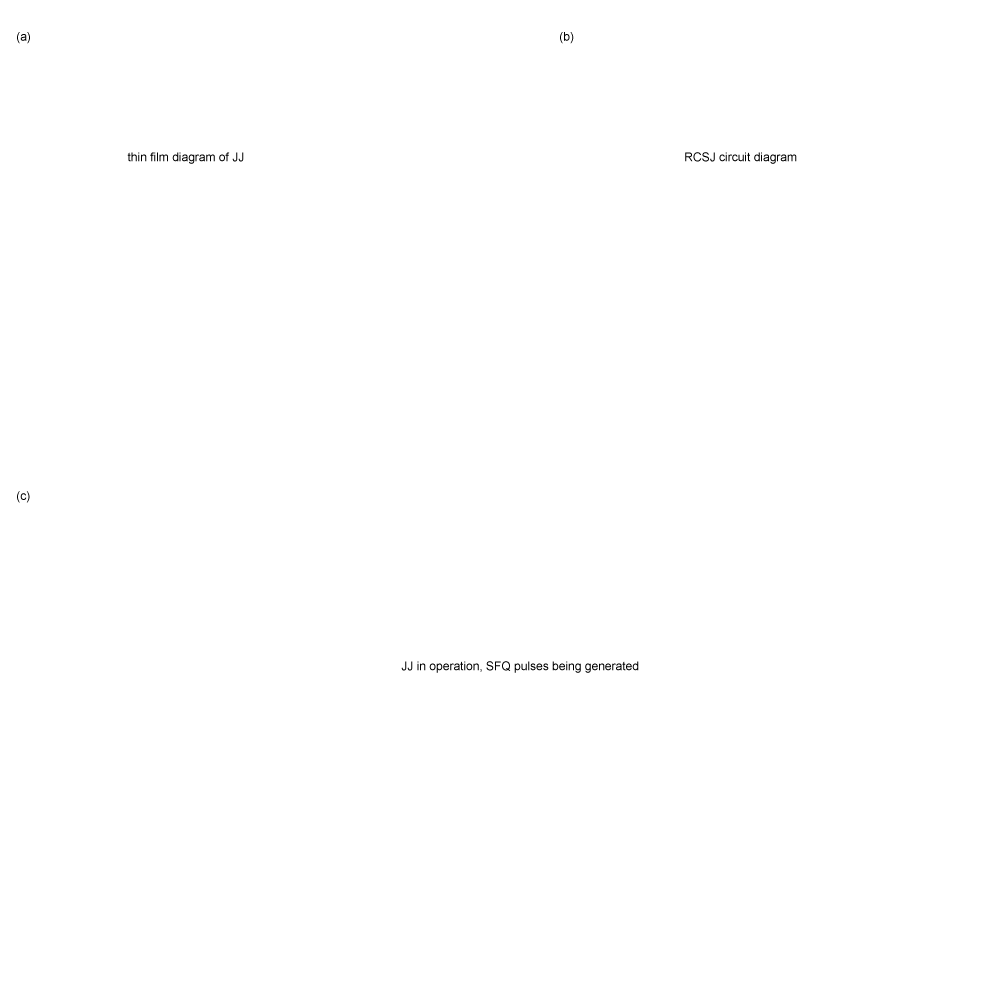
\includegraphics[width=8.6cm]{figures/jj.png}}
	\captionof{figure}{\label{fig:jj}Caption for JJ.}
\end{figure}
A JJ is created when two superconducting wires are separated by a thin tunneling barrier, as shown in Fig.\,\ref{fig:jj}(a). Excellent resources exist that describe the beautiful physics of JJs pedagogically \cite{ti1996,vatu1998,ka1999}, and it is our intention here to describe only very basic aspects of JJ operation relevant to the computing technology under discussion. 

When realized in hardware, any Josephson junction has some shunting capacitance and resistance, leading to the effective circuit shown in Fig.\,\ref{fig:jj}(b), which is referred to as the resistively and capacitively shunted junction (RCSJ) model. While a JJ can, in general, be either voltage biased or current biased, for simplicity we restrict our attention to current-biased junctions as they are more relevant to the operations at hand. One can see that in this model of the junction, there are three conduction paths in parallel. Perhaps the most important aspect of a JJ when used as a classical information-processing element is the fact that the junction has a critical current. This means the central, superconducting path can carry a current $I\le I_{\mathrm{c}}$ with exactly zero resistance and therefore zero voltage acorss the junction. However, if the current bias exceeds $I_{\mathrm{c}}$, the fraction $\Delta I = I-I_{\mathrm{c}}$ cannot be carried through the superconducting channel, and instead must be carried through the parallel conduction pathways, with DC components being shunted through the resistor. Under a bias exceeding $I_{\mathrm{c}}$, a voltage develops across the junction, and in general, this voltage will vary with time, even if the bias is constant, as we will describe in more detail shortly. 

One of the reasons JJs are so fascinating is that depending on the choice of circuit parameters, JJs can demonstrate many behaviors. Because a JJ has an intrinsic inductance, the circuit effective JJ circuit of Fig.\,\ref{fig:jj}(b) can operate as an $L-R-C$ oscillator circuit, leading to ringing behavior. Alternatively, with other parameter choices, the junction can demonstrate latching behavior, wherein a junction biased above its critical current will enter the resistive state and stay there until the current bias is dropped well below the critical current, thus exhibiting hysteresis. For the information processing applications under consideration, it is more advantageous to operate near critical damping.

Let us now consider the operation of a simple circuit employing a single JJ...

Need to touch on speed, flux quantization (need to introduce SFQ terminology, fluxon), JTL, flux storage, energy, $\Phi_0$, integral Vdt

\subsection{Superconducting digital logic}
Here we briefly review the history of using superconductors in digital computing. More detail can be found in Ref.\,\cite{li2012}. The origin of superconducting computing is nearly concurrent with the origin of the rest of digital computing. In that post WWII context, the first components developed were switches for digital systems. The goal was to implement a von Neumann architecture, the same pursuit as vacuum tubes and transistors. In was in this setting that Buck developed a switch wherein a superconducting wire with high critical field is wrapped around a superconducting wire with lower critical field. A current passing through the coil wire could be used to break superconductivity in the core wire. Such an element could be used for switching and current amplification. Dudley Buck referred to this device as a cryotron.

The cryotron was a strong candidate as a switch for binary computing when compared to vacuum tubes, but with the development of integrated circuits this bulk component was not competitive for scaling. Yet in the late 1960s and early 1970s, IBM developed an integrated circuit element based on JJs that behaved like Buck's cryotron \cite{an1980}. At that time, the materials for implementing superconducting integrated circuits were immature, and the device concepts for information processing were also under development. IBM chose to use Pb alloys as the material platform, and they chose to implement a latching logic \cite{lise1991}. This material platform was problematic, and nearly all contemporary efforts in superconducting logic utilize Nb as the predominant material for wiring and JJs (superconducting qubits are primarily based on Al). The latching logic IBM employed used the voltage across a JJ to represent information. As described above, a current-biased JJ can develop a voltage if the current bias exceeds $I\le I_{\mathrm{c}}$, and with a certain choice of the RCSJ circuit parameters, that junction can remain latched in the voltage state even after the current bias drops below $I\le I_{\mathrm{c}}$. Both the choice of Pb as a material platform and the choice to employ voltage-state logic ended up being problematic for IBM, and by the early 1980s IBM ceased its effort in superconducting digital logic.

The effort at IBM began before silicon microelectronic technology had far surpassed other approaches to digital logic, Moore's law had only recently been formulated \cite{mo1965}, and it certainly was not obvious which hardware would dominate for electronic computing. One of the motivations to use superconducting circuits was that they were simpler to fabricate than semiconducting circuits. Additionally, due to the intrinsic dynamics of JJs, they could be made to operate at extremely high speed with low energy per operation. Materials improvements led to the development of JJs based on Nb with AlO$_{x}$ as a tunneling barrier, and several efforts continued to explore JJ-based circuits for computing. In particular, the work by Likharev and others in the late 1980s and early 1990s developed a new type of logic for digital computing (see Refs.\,\cite{lise1991} and \cite{buli2001} for technical details and Ref.\,\cite{li2012} for a retrospective). Within this framework, the state of flux within a superconducting loop represents information: an empty loop represents a binary zero; a loop with one fluxon represents a binary one. This form of logic is referred to as flux-state logic, and it overcomes many of the weaknesses of voltage-state logic. Likharev and colleagues referred to this approach as rapid single-flux-quantum logic, and developed a family of gates to implement digital computing. Within this framework, a clock is distributed across all gates in the system, and logical operations proceed based on whether or not flux is present in certain loops during each clock cycle. 

The foundational work on flux-state logic \cite{lise1991,buli2001,li2012} occurred during the prime years of silicon microelectronic scaling. For this reason, it was difficult to foster a large effort in a competing technology, leading Likharev to later lament the oppressive impact incurred on other technologies as ``CMOS continued its victorious march.'' \cite{}. Yet interest in superconducting electronics for computing has continued, particularly in Japan, and as the scaling of silicon transistor technology has reached new barriers, attention has returned. In the US, the resurgence led to the IARPA Cryogenic Computing Complexity program, started in 2014, to develop high-performance superconducting digital computers. This effort, however, has not quickly led to circuits outperforming CMOS for digital computing. There are four reasons for this. We list them in order of severity. The first reason is that it is difficult to implement large arrays of compact memory cells with superconducting electronics \cite{}. This is very problematic when implementing the von Neumann architecture, as these digital efforts have aspired to do. The secondary reason is that distribution of a high-speed clock across many logic gates encounters obstacles, and the timing jitter of the gates leads to errors if the clock is too fast, largely eliminating speed advantages relative to CMOS. The third reason is that a superconducting system resides inside a cryostat. A high-performance computer will need extensive I/O, and this cannot be achieved straightforwardly with co-axial cables due to the high heat load such cables transfer from room temperature the the 4.2\,K stage where computation is performed. Optical approaches are being developed to overcome this challenge \cite{}, but optical sources or modulators often require on the order of a volt to encode a bit, while the SFQ pulses produced by JJs are on the order of a millivolt. This introduces the fourth problem limiting the success of superconducting electronics for digital computing: it is difficult for a superconducting circuit to change the state of a CMOS circuit. That is to say, it is difficult for a superconducting circuit to achieve sufficient voltage to switch the gate of a silicon transistor. Even if one intends to develop superconducting electronics to outperform silicon electronics specifically in the domain of digital logic, it is helpful (and perhaps vital) that the superconducting system be able to interface bi-directionally with semiconductors so the superconducting system can leverage the tremendous infrastructure of semiconductor integrated circuits. 

\vspace{3em}
still need in this section:
\begin{itemize}
\item description of RQL
\item description of AQFP, extreme energy efficiency, Landauer limit
\end{itemize}

\vspace{3em}
recent work on basic science of MJJs: cama2018,kamu2018,bakl2018
search bib for MJJ

\vspace{3em} 
discussion of superconducting electronics for sensing/particle detection

\vspace{3em}
Superconducting circuits can perform Boolean logic well enough to control networks of loop neurons and possibly qubits, but superconducting electronics are not poised to displace CMOS electronics for logic, particularly not in lightweight applications such as IoT and edge computing that have become so influential to the development of hardware for AI. 

\subsection{Superconducting optoelectronic neural systems may overcome challenges of digital systems}
Let us refer to these challenges with superconducting electronics as: 1) the memory problem; 2) the clock problem; 3) the I/O problem; and 4) the volt problem. We will argue below that a new type of cryotron, implemented in a compact, on-chip, thin-film device can overcome the volt problem, but only if one accepts slower speed than superconducting digital logic seeks, an acceptable trade-off in a neural system. Solving the volt problem this way enables us to generate light, thereby solving the ``O'' part of the I/O problem. The ``I'' part of the problem is solved by utilizing superconducting photon detectors, compact circuit elements developed since 2000 and integrated with photonic circuits within the last decade. With integrated light sources and detectors, superconducting systems can send and receive near-infrared photons over optical fibers, relieving the heat load of co-axial cables, and solving the volt problem at semiconductor photodetectors on the room-temperature side. The asynchronous nature of spiking neural systems eliminates the clock problem, provided synaptic, dendritic, and neuronal integration times can be made longer than the jitter of the circuits. Finally, while the memory problem is the most severe for superconducting digital systems, the prospects for memory in superconducting neural systems are one of the most exciting aspects of the technology. As discussed in Sec.\,\ref{sec:neuroscience}, memory in neural systems involves short-term plasticity, long-term plasticity (STDP, for example), and metaplasticity (that adapts the rate with which synapses change). We find that JJ circuits very naturally implement these functions, and the distributed nature of synaptic memory avoids the difficulty of creating large arrays of addressable superconducting memory elements. 

We will describe these superconducting optoelectronic circuits in more detail in Sec.\,\ref{sec:optoelectronicNeurons}. Let us first turn our attention to JJ circuits that implement neural functions without optical communication.

\subsection{Neurons based on Josephson junctions}
The development of superconducting digital electronics in the 1980s and 1990s was concurrent with the second wave of excitement regarding neural networks. Thus, several research groups developed circuits based on JJs to behave as neurons in ANNs, primarily in Japan. Following two conference proceedings in 1989 \cite{ai1989,og1989}, the first articles regarding JJ circuits for ANNs were published in 1991 \cite{hago1991,hiak1991}. The objective of the circuits was to perform the weighted summation and thresholding operations required in the computational primitives of ANNs. The circuits employed were similar to those utilized in superconducting digital logic, as were the basic concepts, such as using an up-down counter to implement synaptic weights \cite{hiak1991}. From the beginning, attention was paid to sculpting a sigmoidal transfer function to implement back-propagation as well as alternative circuits for achieving Hebbian-type learning \cite{hago1991}. The intrinsic threshold of a JJ upon being driven above its critical current was naturally used for thresholding \cite{hago1991}, and mutual inductors were identified as promising for addition of synaptic signals and fan-in \cite{hiak1991}. Little analysis was dedicated to anticipating scaling of such systems, although Ref.\,\onlinecite{hiak1991} claimed that achievable fan-out would be ``sufficiently large to implement large scale neural networks,'' and that ``fan-in is essentially unlimited.'' While the first assertion depends on one's definition of ``large scale'', subsequent analysis indicates that fan-out is a serious fundamental challenge for superconducting electronics, and fan-in reaches practical limitations due to the properties of mutual inductors, as we will discuss in more detail below.

Subsequent designs and experimental demonstrations were presented by Mizugaki et al. in 1994 \cite{mina1994a,mina1994b} and 1995 \cite{mina1995}. These circuits employed SQUIDs in various configurations for synaptic and neuronal responses. Again, digital concepts were employed, such as establishing the bit depth of possible synaptic weight values by adding additional DC SQUIDs. The focus remained on achieving feed-forward ANNs. Regarding fan-out, the intention was to use direct connections via superconducting wires to communicate between neurons. As stated in Ref.\,\onlinecite{mina1994a}, ``If it is necessary for a neuron circuit to drive a lot of another neurons, we can use biased JTLs...though the use of JTLs might reduce the integration scale.'' 

In 1997 Rippert and Lomatch at Northwestern University proposed neural circuits using similar principles of SFQ pulse generation rate representing activation, but new innovations were introduced regarding learning \cite{rilo1997}. The emphasis was still on ANNs rather than spiking neurons, and digital circuits were employed wherein higher-bit-depth synapses were achieved by adding junctions. This work began to explore Hebbian learning based on the temporal coincidence between two fluxons incident upon a JJ. In their circuit design, the coincidence window is determined by the temporal width of fluxons as well as the JJ bias current, and could achieve values of 1\,ps to 5\,ps. Reference \onlinecite{rilo1997} was the first to introduce a mechanism for metaplasticity in superconducting synapses wherein synaptic efficacy is updated through a Hebbian process, and the rate of Hebbian update is modified by additional circuits that adapt the Hebbian circuits. This work was before the term ``metaplasticity'' had become common in the neuroscience literature, but after the 1982 introduction of the BCM learning rule \cite{bico1982} that some consider the first example in computational neuroscience of a metaplastic synaptic mechanism \cite{cube2012}.

Efforts in superconducting neural circuits continued in Japan through the 2000s and 2010s \cite{koko2005,onko2009,hias2006,hias2007,onma2011,yaum2013}. The emphasis remained on ANNs implemented with circuits originally designed for digital logic. References \onlinecite{koko2005} and \onlinecite{onko2009} continued to explore and demonstrate the approach with up/down counters to represent a membrane potential with the output rate of fluxons representing the neuron's activation. Networks of these circuits were simulated solving a combinatorial optimization problem in Ref.\,\onlinecite{onma2011}, and more attention was paid to generating an accurate sigmoid function for back-propagation in Ref.\,\onlinecite{yaum2013}. In 2013 in Italy, a small network of SQUID-based neurons was demonstrated and used to implement an XOR gate when trained through examples using an genetic algorithm in Ref.\,\onlinecite{chca2013} .

Throughout Refs.\,\onlinecite{hago1991,hiak1991,mina1994a,mina1994b,mina1995,rilo1997,koko2005,onko2009,onma2011,yaum2013}, a neuron's activation was represented by the rate of production of fluxons, which becomes the time-averaged output current after low-pass filtering. By contrast, Refs.\,\onlinecite{hias2006} and \onlinecite{hias2007} proposed designs for leaky integrate-and-fire neurons that sum fluxons and produce a single flux quantum upon reaching threshold, much more in the spirit of single-flux-quantum digital electronics. To my knowledge, this was the first proposal to use superconducting circuits for spiking neurons. Input fluxons were stored in superconducting loops, and the number of input fluxons required to reach threshold was set in hardware by the number of JJ storage loops in the integrator. The leak rate was established by adding a resistance to one of the loop, giving exponential current decay with an $L/r$ time constant. Fan-out was envisioned to occur through JTLs and splitters, while fan-in was envisioned to utilize confluence buffers. No scaling analysis regarding the possible number of connections was presented.

In 2010, Crotty, Schult and Segall at Colgate University proposed a different approach to integrate-and-fire neurons \cite{crsc2010}. Rather than focusing on achieving weighted summation and nonlinear activation for ANNs, this work was oriented toward using JJ circuits to model neurons and their dynamics. Toward this end, they also adapted a circuit from superconducting digital electronics. The neuron circuit proposed in Ref.\,\onlinecite{crsc2010} is based on the DC-to-SFQ converter. Segall and his colleagues identified a correspondence between the behavior of each of the two junctions in the circuit and ionic currents across a neuron's cell membrane, with one junction behaving like a Na$^+$ current producing the rise of an action potential, and another junction behaving like a K$^+$ current quenching the action potential and restoring the membrane potential to its resting level. It was estimated that a cortical column with $10^4$ neurons could be simulated with JJ circuits on a single chip, but an interconnection scheme was not proposed. Subsequent work from the Colgate group simulated \cite{segu2014} and experimentally realized \cite{sele2017} synchronization dynamics of a two coupled neurons. In these neurons, a pulse consisting of a single flux quantum represents an action potential, and an RC circuit achieves synaptic leak, resulting in neuronal firing up to 25\,GHz with $10^{-17}$\,J/spike. 

While 10\,aJ per action potential is low, some aspire to far lower operation. As mentioned in Sec.\,\ref{sec:superconductors}, there are multiple ways to use JJ circuits to implement digital logic. Correspondingly, there are multiple ways to use similar circuits to implement neural functions. While much of the work on superconducting neurons utilizes circuits most similar to SFQ logic circuits, an emerging branch utilizes AQFP circuits (see Sec.\,\ref{sec:superconductors}). The energy efficiency of AQFP circuits derives from the fact that the junctions involved are never driven above their critical current, and so never produce fluxons. Instead, the Josephson nonlinear inductance is employed to establish nonlinear current input/output relations. Utilization of adiabatic cells for ANNs was first introduced in 2016 by Schegolev et al. in Russia \cite{sckl2016}, and the ideas have been further developed in Refs.\,\onlinecite{klsc2018} and \onlinecite{sosc2018}, where the authors proposed to utilize MJJs for synapses in conjunction with adiabatic neurons.  Work from Katayama et al. in Japan \cite{kafu2018} has developed related concepts flux-biased SQUIDs to achieve a sigmoidal transfer function suitable for back-propagation for training ANNs.

As mentioned in Sec.\,\ref{sec:superconductors}, Josephson junctions with a ferromagnetic material in the tunneling barrier can be used as a memory element in superconducting circuits \cite{vevi2013}. The state of magnetic order can be used to tune the critical current across a broad range, and this can be used to steer a bias current. The use of MJJs as a synapse in superconducting neural circuits was first proposed in 2016 by Russek et al. \cite{ru2016} and has been subsequently demonstrated by Schneider et al. \cite{scdo2018} in 2018. Further theoretical analysis of the use of MJJs for establishing synaptic weights in ANNs based on similar SQUID neurons to those discussed above \cite{hiak1991} was presented Ref.\,\cite{scdo2018b}, wherein simulation of nine-pixel image classification was shown with 3\,ns inference time per image. 

While all superconducting electronic neural systems mentioned in the section have utilized circuits based on JJ and their associated nonlinearities and thresholding behavior, neuron circuits based on quantum phase-slip junctions (QPSJs) have also recently been proposed \cite{chgo2018}. QPSJs are the dual to JJs, and thus corresponding dual circuits can be conceived to perform neural functions. QPSJs also have thresholding behavior and may offer further advantages in energy efficiency. These devices are still being developed, and one technical challenge is that one-dimensional superconducting wave functions must be achieved, which requires lithography down to about 10\,nm, making initial demonstrations as well as future scaling potentially more difficult than with JJs.

\subsection{Strengths and weaknesses of JJ circuits for neural operation}
In Refs.\,\onlinecite{hago1991,hiak1991,mina1994a,mina1994b,mina1995,rilo1997,koko2005,onko2009,hias2006,hias2007,onma2011,yaum2013,crsc2010,segu2014,sele2017,sckl2016,klsc2018,sosc2018,ru2016,scdo2018,scdo2018b,chgo2018}, five arguments have been forth regarding why superconducting circuits might outperform semiconducting circuits for neural computing: 1) JJs are faster than transistors, so JJ neurons and synapses will be faster than their silicon counterparts; 2) JJs consume less energy per operation than transistors, so superconducting neural systems will be more energy efficient; 3) JJs are highly nonlinear and have native thresholding and spiking behavior, so synaptic and neuronal circuits based on JJs can be implemented simply with few JJs; 4) superconducting transmission lines are lossless, so communication in superconducting neural systems will be superior to semiconducting neural systems using normal metal interconnects; and 5) due to their low power density, superconducting devices can be stacked in three dimensions with multiple planes of JJs, whereas the difficulty of removing heat from transistors precludes multiple active layers in a CMOS process. While I am a proponent of using JJ circuits for synaptic and neuronal functions, these arguments do not all hold up to scrutiny. As a broad comment, nowhere in Refs.\,\onlinecite{hago1991,hiak1991,mina1994a,mina1994b,mina1995,rilo1997,koko2005,onko2009,hias2006,hias2007,onma2011,yaum2013,crsc2010,segu2014,sele2017,sckl2016,klsc2018,sosc2018,ru2016,scdo2018,scdo2018b,chgo2018}, is a system-level analysis of a large network presented. Neural systems are complex with many device and circuit interdependencies across various scales of the network. To analyze claims about full systems based on the performance of a device in an isolated context can be misleading. To further illustrate these issues, let us consider each of the above arguments.

\vspace{1em}
\textit{1) JJs are faster than transistors, so JJ neurons and synapses will be faster than their silicon counterparts.} \newline It is true that the intrinsic time constants of JJ are shorter than transistors. Yet the cutoff frequency of a transistor does not limit the speed of CMOS neural networks directly. Because CMOS neural networks have reached a sufficient stage of maturity, full, functional systems can be analyzed. We find that at the scale of 100,000 neurons, event rates are limited to 1\,kHz per neuron \cite{payu2017}, and by 100 million neurons it is limited to 10\,Hz \cite{kuwa2017}, and this poor scaling results from the communication infrastructure, not the elemental device speed. It may be possible that large networks of JJ neurons are faster than large networks of transistor neurons, but we cannot conclude this until we know how communication will occur in these networks.

\vspace{1em}
\textit{2) JJs consume less energy per operation than transistors, so superconducting neural systems will be more energy efficient.} \newline At the device level, this argument seems well-founded, especially if adiabatic principles of operation are employed. Yet again we must think at the system level. The power required to operate a system at 4\,K in a background at 300\,K can be modeled as
\begin{equation}
\label{eq:power_to_operate_cryo}
P_{\mathrm{tot}} = m P_{\mathrm{dev}} + P_{\mathrm{0}},
\end{equation}
where $P_{\mathrm{dev}}$ is the power dissipated by the devices comprising the system due to normal operation, and $P_{\mathrm{0}}$ is the power required simply to cool the devices below to the operating point, which is 4\,K for most superconducting systems under consideration for this form of computation. This power is at least 100\,W for contemporary cryogenic systems, and is often 1\,kW, even when there are zero neurons in the system. The slope $m$ represents watts of cooling power required to stay below 4\,K per watt of device power dissipated due to operation. The theoretical limit is given by the Carnot efficiency, and when cooling from 300\,K to 4\,K this number is 150 watts per watt. In practice, it is often approximated as 1000 watts per watt. Thus, if we plan to operate the artificial neural system on earth, we should budget 1\,kW of power just to turn it on, and we should budget an additional 1\,kW of system power for each watt dissipated by the devices. This clearly limits the application spaces where superconducting systems are candidates to outperform semiconducting systems with regard to power consumption. Much of modern AI hardware aspires to play a role in small, deployable devices. Superconductors will never be useful in cell phones, the internet of things, or edge computing. Systems based on JJs may be more efficient than systems based on transistors, but this will only become relevant for systems large enough that the term $P_{\mathrm{0}}$ is tolerable. The domain of superconductors in neuromorphic supercomputing. High-$T_{\mathrm{c}}$ materials are unlikely to change this situation because the materials involved make fabrication of dense, integrated circuits very difficult, and operating of JJs at higher temperature is very noisy, even if the underlying material has a high $T_{\mathrm{c}}$ \cite{lise1991} (check this ref). 
  
  \vspace{1em}
\textit{3) JJs are highly nonlinear and have native thresholding and spiking behavior, so synaptic and neuronal circuits based on JJs can be implemented simply with few JJs.} \newline To me, this is the most compelling argument in favor of superconducting neural systems. Josephson junctions are ideal for performing the synaptic, dendritic, and neuronal behaviors we seek. This is most apparent when implementing spiking neurons that fully utilize the time domain. Most of the work to date in superconducting neural circuits has focused on generating nonlinear transfer functions, essentially for steady-state operation in feed-forward neural networks \cite{hago1991,hiak1991,mina1994a,mina1994b,mina1995,rilo1997,koko2005,onko2009,onma2011,yaum2013,sckl2016,klsc2018,sosc2018,ru2016,scdo2018,scdo2018b,chgo2018}, but we will argue in Sec.\,\ref{sec:superconductingOptoelectronic} that JJ circuits similar to the spiking neurons of Segall and co-workers \cite{crsc2010,segu2014,sele2017} can perform many desirable synaptic, dendritic, and neuronal functions going far beyond simple, point-neurons.

\vspace{1em}
\textit{4) Superconducting transmission lines are lossless, so communication in superconducting neural systems will be superior to semiconducting neural systems using normal metal interconnects.} \newline The dissipationless nature of superconducting wires is an extraordinary benefit to neural computing, digital logic, and quantum computing alike. But dissipationless transmission lines alone are not sufficient to enable an interconnection network, particularly when spiking is involved. The major problem with communication on metal wires is not resistance, but capacitance, as described in Sec.\,\ref{sec:electronics}. Likewise, superconducting interconnects must contend with problems related to inductance. If the output of a neuron is one or more fluxons generated by a JJ, the current associated with each fluxon will be $\Phi_0/L$, where $L$ is the total inductance of the output lines being fed by the JJ. As more connections are added, the inductance gets larger, the current gets smaller, and the neuron eventually cannot source enough current to directly feed all of its synaptic connections. One solution to this problem is to use JTLs and pulse splitters to provide gain as a pulse porpagates through and branches across the interconnection network. Other approaches to fan-out are discussed in Sec.\,\ref{sec:superconducting_interconnects}, but it is likely that an active interconnection network of JTLs and splitters will be required to achieve communication from one spiking neuron to many synaptic connections. Active transmission lines dissipate power, and so arguments related to the lossless nature of superconducting transmission lines are not applicable. Again, one must propose an interconnection network adequate at the system level to assess the full benefits of lossless communication lines. It is not clear that routing of fluxonic signals from JJ neurons across large networks can be achieved without resorting to address-event representation, as is done by CMOS. If AER proves necessary, superconducting circuits will have much more difficult road ahead than CMOS, because AER places severe demands on memory, and superconducting circuits struggle with dense memory.

For certain feed-forward superconducting ANNs, particularly those based on AQFP circuits, it is not necessary for a neuron to produce an output that switches a junction, and passive transmission lines with high inductance may suffice. In this case, the high inductance will lead to reduced speed when changing the inputs to the network, so the interconnection network must be analyzed in conjunction with the inference latency, and speed/scaling trade-offs will be present.

\vspace{1em}
\textit{5) Due to their low power density, superconducting devices can be stacked in three dimensions with multiple planes of JJs, whereas the difficulty of removing heat from transistors precludes multiple active layers in a CMOS process.} \newline This could be another tremendous advantage of superconducting circuits for long-term scaling. The power density of JJ circuits is low enough that many layers could be stacked while maintaining the ability to conduct heat to a bath of liquid helium, particularly when the circuits are participating in temporally sparse neural activity. However, in practice it is difficult to produce wafers with multiple planes of JJs \cite{to2016}, although there is plenty of room for development through future research. Three-dimensional integration of complex JJ neural circuits appears possible in principle, and it remains to be seen how far it can go in practice, but if successful could bring exceptional advantages for large-scale systems.

\vspace{1em}
In this section we reviewed 30 years of work on superconducting neural circuits, and we described their strengths as well as their weaknesses. 

\vspace{1em}
\begin{itemize}
\item mina1994a anticipated problems with superconducting lines, JTLs, and scaling
\item early works used digital concepts, adding active circuits to increase synaptic bit depths, hwereas we now plan to use purely passive Lr loops, enabled by high-kinetic-inductance materials
\item neuronal firing: mina1994a, mina1995, hagu1991 all use time-averaged output of SFQs from JJ as signal representing activation (not 1 fluxon action potential)
\item advantages of superconductors for 3D integration seen in hiak1991
\item temporal coincidence: compare/contrast with rilo1997 where use $\Delta t$ of JJ. also metaplasticity
\end{itemize}

\section{\label{sec:superconductingOptoelectronic}Superconducting optoelectronic systems}

%\cite{kafe2015} Waveguide integrated superconducting single-photon detectors with high internal quantum efficiency at telecom wavelengths

These detectors are wires of superconducting material \cite{mave2013}, and they can be straightforwardly patterned atop on-chip dielectric waveguides \cite{shbu2017b,x,y,z}. The nanowire thickness is 4\,nm-10\,nm, its width is 80\,nm-350\,nm, and the interaction length along the waveguide can be as short as 10\,\textmu m. The wire is current biased in parallel with a resistive load (Fig.\,\ref{fig:snspd}), .

Because the detectors are superconducting, they draw very near zero power in the steady state. 



\begin{itemize}

\item general concept: communication between neurons is photonic; when a neuron spikes it must either generate or modulate light; throughout, speed, size, power all co-optimized

\item first key choice: generate or modulate

\item modulate:
\begin{itemize}
\item requires cw light running at all times ($x_{dB/cm} = 1; y_{dB/s} = 100*x_{dB/cm}*c; q_{dB} = 3; t_s = q_{dB}/y_{dB/s}$, for 1\,dB/cm propagation loss, 3\,dB of the light is lost every 100\,ps)
\item requires frequency tuning, most likely
\item cross talk of neurons on the same bus
\end{itemize}

\item generate:
\begin{itemize}
\item requires light source at every neuron
\item requires unprecedented optoelectronic integration, million sources and a billion detectors on a wafer
\item must be very low capacitance
\item seems like only a silicon light source will suffice, but this would require cryogenic operation
\end{itemize}

\item second key choice: establish synaptic weight in the photonic or electronic domain?

\item photonic domain:
\begin{itemize}
\item This choice has several important ramifications for hardware and information processing. Regarding information processing, it is usually assumed that neural communication is digital: the presence or absence of an action potential is a binary one or zero, and the amplitude of the action potential is not encoding information. When adjusting the synaptic weight in the photonic domain, this is not the case. The number of photons reaching a neuron through a synaptic connection becomes an analog variable, and it is subject to shot noise, in addition to any noise mechanisms present in the detector. The signal-to-noise ratio of shot noise improves with $\sqrt(N_{\mathrm{ph}})$, where in this case $N_{\mathrm{ph}}$ is the average number of photons, so establishing weights in the photonic domain introduces an energy/noise tradeoff. Setting weights in the photonic domain also has the disadvantage that photons are discarded by attenuation at weak synaptic weights. Thus, by setting synaptic weights in the photonic domain, we place a burden on light sources to produce large numbers of photons to minimize shot noise, and we discard photons when they are attenuated at weak synapses. In this mode of operation, light is used for communication, but it is also used for the important computational operation of applying the synaptic weight.
\item these objections notwithstanding, to our knowledge, all except one optoelectronic neural approach proposed to date sets weight in photonic domain
\item specific instances: mzi (no STDP, poor spatial scaling, cross-talk); wdm (limited number of channels, cross-talk with rings on master ring, demands on sources); mzi and wdm (thermal tuning hopeless for scaling, no plasticity mechanisms proposed); phase change synapses (at least don't dissipate steady state, still power lost due to variable attentuation, small footprint, Hebbian learning possible, but STDP not likely, meta, short term also doesn't look promising)
\end{itemize}

\item electronic domain:
\begin{itemize}
\item By contrast, if we establish synaptic weights in the electronic domain, light is used exclusively for communication, and communication remains entirely digital. The presence of an optical signal can be used to represent an all-or-none communication event. In this case, the detector and associated electronics must be able to achieve a variable synaptic response to identical photonic pulses based on the configuration of the electronic aspects of the circuits. In this case, we expect that a neuron will send, on average, $N_{\mathrm{ph}}$ photons to each of its downstream synaptic connections. Due to shot noise, each downstream connection will receive $N_{\mathrm{ph}}\pm\sqrt{N_{\mathrm{ph}}}$ photons, and the detector circuit must be configured to implement a synaptic response if a threshold of $N_{\mathrm{th}}$ photons is detected. After detection, the electronic response must vary depending on the synaptic weight, independently of the precise number of photons that was detected. It is in this electronic response that the signal becomes analog again. Whereas setting the synaptic weights in the photonic domain places a larger burden on light sources, setting the synaptic weights in the electronic domain places a larger burden on detector circuits. One must achieve a detector circuit that converts light pulses to electrical current or voltage, and the amount of electrical signal must be largely independent of the number of photons in the pulse, depending instead on reconfigurable electrical properties of the circuit, such as bias currents or voltages. These reconfigurable bias currents or voltages then represent the synaptic weights, and the task of a neuron's light source is simply to provide a roughly constant number of photons to each of its downstream synaptic connections. For energy efficiency, the number of photons necessary to evoke a synaptic response from the detector ($N_{\mathrm{th}}$) should be made as low as possible to make the job of the light source as easy as possible. $N_{\mathrm{th}}$ cannot be made lower than one, as the electromagnetic field is quantized into integer numbers of photons.
\item only know of one system where electronic domain has been proposed: soens
\item basic functionality
\item stdp
\item meta
\item homeo
\item short-term
\end{itemize}

\item neuronal computation: reaching threshold
\begin{itemize}
\item differentiate between state-based and spiking
\item main considerations here are energy/power
\item how much energy is required to generate a pulse or drive a modulator? 
\item how much light must be made/moved to drive all downstream synaptic connections? 
\item how fast can pulses be generated (refractory period)? 
\item how long can neurons remember (leak rate)? 
\item what is range of spike rates? what is expected power?
\end{itemize}

\item somewhere in here, comparison of detectors (going cold costs 500x for carnot, but gains 2000x for detector sensitivity)
\item related, comparison of sources (going cold reduces how many photons must be made, but most importantly, if it means a silicon light source can work for this project, it is a game changer)

\item inhibition, gotta have a plan

\item dendritic processing
\begin{itemize}
\item intermediate nonlinearities
\item direction attention with inhibition
\item sequence detection
\item how can any of this happen in the photonic domain?
\end{itemize}

\item room temp vs cryo
\begin{itemize}
\item sources (cryo enables Si sources. for large-scale integration, process simplicity brings tremendous advantage)
\item detectors (A SiGe photodetectors needs about $10^4$ photons in 100\,ps to respond; efficiency of SNSPDs, low-noise of SNSPDs, simplicity of fabrication, and excellent operation in conjunction with JJs)

\end{itemize}

\end{itemize}

\section{\label{sec:scaling}Large-scale optoelectronic systems}

\subsection{Criteria for assessing cognitive neural hardware}
\begin{itemize}

\item network metrics
\begin{itemize}
\item total number of neurons in network
\item degree distribution
\item clustering coefficient on different scales
\item average network path length
\item modularity analysis
\item rentian analysis
\end{itemize}

\item synaptic metrics
\begin{itemize}
\item range of achievable synaptic weights
\item number of achievable synaptic weights
\item max synaptic state retention time
\item analysis of short-term plasticity responses (filter properties, energy consumed, area)
\item analysis of stdp (range of values, update rates, energy required, time window control, area required)
\item analysis of metaplasticity (mechanisms, range of rates, energy required, area required)
\item total size of synapse
\end{itemize}

\item dendritic metrics
\begin{itemize}
\item analysis of dendritic intermediate nonlinear processing (range of time scales, I/O (gain) curves, energy, num synapses per dendrite, operations performed)
\item analysis of dendritic sequence detection (time scales, number of synapses involved, energy)
\item available logic operations (Boolean, time of last firing, multisynaptic)
\item number of values achievable in readout
\item size of dendrites
\end{itemize}

\item neuronal metrics
\begin{itemize}
\item total number of dendrites
\item total number of synapses
\item analysis of the rentian fan-in of the dendrito-synaptic arbor
\item dynamic properties of threshold
\item refractory period
\item integration time (if different from dendritic integration)
\item energy of neuronal firing
\item timing jitter of neuronal firing
\end{itemize}

\item communication metrics
\begin{itemize}
\item total system bandwidth (at neuronal level, also including dendritic level where neuronal data rates are multiplied by information available to first layer of dendrites after any additional synaptic fanout)
\item I/O 
\end{itemize}

\item system operation metrics
\begin{itemize}
\item operating temperature
\item power consumption
\item max spike events per second
\item power consumed during max spike events per second
\item power density
\item temperature variation during operation
\item total system size
\end{itemize}

\item system production metrics
\begin{itemize}
\item equipment required (i.e., technology node)
\item device yield/tolerance to variation
\item time required
\item packaging strategy
\item total material consumed
\item total cost to produce 
\end{itemize}

\end{itemize}

\begin{itemize}
\item unprecedented integration of photonics and electronics in a scalable process that can be implemented with existing infrastructure--change a few implant conditions, swap out a few sputtering targets, improve BEOL dielectrics for photonics
\item communication on various length scales, multi-planar on wafers, wafer-to-wafer vertical and lateral, fiber white matter
\item feasibility of brain scale
\item why si if no transistors?
\begin{itemize}
\item III-V substrates should be pursued as well. Our group is working on this, initial anecdata indicates similar efficiency
\item big problem is fab. wafers are harder to scale, material harder to purify, oxide not as good for waveguide cladding. Similar consideration to mosfet gate. Overall manufacturability
\item may eventually use transistors for perhaps faster refractory period
\end{itemize}
\item ultimate limits
\end{itemize}


For general networks, the algorithm by which partitions are identified can be made mathematically rigorous from a network theory perspective \cite{oz1992,oz2004}. For the analysis at hand, we consider the partitions of the network we have assigned in the hierarchy. For example ... (minicolumns, mesocolumns, macrocolumns on a wafer(s); multi-columnar modules, ...) 
\subsection{Achieving hierarchical modularity}

\subsection{Integrated systems across temperature stages}

\subsection{Optimal environment for operation: the asteroid belt}



\section{\label{sec:applications}Application spaces}

\begin{itemize}
\item original applications of computing
\begin{itemize}
\item cryptography
\item weather
\item bombs
\item numerical solution to arbitrary diff eqs
\item from Turing, AI
\item now, apply to nearly all aspects of modern life
\end{itemize}
\item what others in the field are pursuing
\begin{itemize}
\item LASSO \cite{dasr2018}
\item fast control \cite{prsh2017}
\end{itemize}
\item here, following neuroscience applications 
\begin{itemize}
\item vision systems
\item language processing
\item motor control
\item may lead to Turing's vision of an AGI one can interact with
\end{itemize}
\item others, unique to large-scale neural systems and/or superconducting optoelectonic
\begin{itemize}
\item internet monitoring/simulation
\item sociological simulation
\item genetic analysis/evo devo
\item neuroscience and dynamical systems
\item quantum/neural hybrid systems (Bayesian discussion)
\end{itemize}
\end{itemize}

\subsection{Hybrid systems}

Modules for specialized processing: deep learning, quantum, high-speed inference, sensory organs

\subsubsection{Neural-deep learning hybrid systems}
Deep learning modules may provide types of sensory inputs, visual system design can borrow from CNNs and bio, olfactory with combs, etc. (cite personal communication)

\subsubsection{Classical-quantum-neural hybrid systems}
Quantum systems and neural systems have complimentary information processing capabilities. Quantum systems are fundamentally probabilistic, while neural systems are excellent for sampling probability distributions. Schemes to utilize quantum information are usually statistical, while populations of neurons can perform optimal Bayesian inference on samples drawn from statistical distributions. This reasoning leads us to consider the potential to utilize a neural system to perform quantum state tomography on large-scale quantum systems. The goals of the project are to construct a neural system capable of: 1) measuring the state of a network of qubits at the Heisenberg limit; 2) inverting the physical measurement through Bayesian inference to arrive at a quantum state reconstruction; and 3) reporting the reconstructed state over a classical communication channel as the qubits evolve in time, all implemented in scalable hardware.

Quantum information processing requires the ability to determine an unknown quantum state from a series of measurements performed on an ensemble of identically prepared systems. Performing measurements on many interacting qubits places severe demands on measurement hardware. To characterize a large quantum system, the number of measurements that must be performed can become intractably large if care is not taken to optimize the measurement protocol [1,2]. Additionally, the computational challenge of reconstructing the full quantum state from the set of measurements is formidable for large quantum systems. Developing hardware with classical, quantum, and neural capabilities presents an alternate route to develop scalable measurement techniques to extract Heisenberg-limited information [3] from a complex quantum system, to devise a method for a full quantum state to be efficiently reconstructed from measured data, and to ensure that the hardware implementation of this measurement/analysis procedure communicates efficiently to room temperature. 

At present, the various elements of scalable quantum state tomography are maturing and beginning to combine. In hardware, control and measurement circuits operating at cryogenic temperature are being developed. Josephson circuits capable of detecting single microwave photons present an exciting new avenue for scalable qubit characterization [4], yet racks of control and readout electronics are still employed for interfacing to relatively small quantum systems. Regarding reconstruction of quantum states from measured data, statistical methods involving Bayesian inference have been developed in the context of quantum tomography over the last 30 years [5-9]. It has been shown that by reoptimizing the measurements to be performed as information about the quantum state is acquired, the total number of measurements can be reduced [10]. Modern techniques in machine learning have been applied to the problem, showing that a neural network can perform quantum state tomography on highly entangled states of a hundred qubits [11]. The neural network employed in the tomographic analysis of Ref. 11 is a conventional, feed-forward neural network implemented in software. The related field of spiking neural networks has found that populations of spiking neurons naturally perform Bayesian inference [12-14]. Networks of spiking neurons can be trained so the average firing rate of the population represents the expectation value of an observable, and the variance of the firing rates of the neurons represents the uncertainty. Bayesian analysis has been applied to a series of weak measurements to track the trajectory of a single qubit, but cumbersome measurement hardware infrastructure was utilized [15]. Software neural nets have been used to perform tomography on 100-qubit systems, but the measurements were performed conventionally [11]. The adaptive Bayesian formalism has been applied to a two-qubit system to minimize the number of measurements required for full state reconstruction, but explicit numerical calculations were performed on conventional computers between each measurement [2]. Spiking neural networks have been used to perform Bayesian inference on statistical distributions [16], but the systems under observation have all been classical [14]. It has been shown that neural networks can emulate quantum computation [17-19], can accurately measure quantum systems [20], and can perform quantum state tomography [11]. The proposed hybrid hardware would combine these advances in a measurement apparatus performing Heisenberg-limited measurements, conducting Bayesian inference in real time as information is received, and using all knowledge about the quantum system for optimization of measurement protocol and full state reconstruction. The metrological hardware we propose to develop would prepare highly entangled states of many qubits, perform the measurements and information processing necessary for tomography, and communicate the results of state reconstruction to room temperature with near-infrared photons over optical fiber [21].

This concept remains in the domain of thought experiments, but we will describe a route to make it real. We propose to model and construct the classical-quantum-neural (CQN) hybrid system depicted schematically in Fig. 1. The system comprises a classical control module, a quantum module containing a network of coupled qubits, and a neural module interfacing with both the classical and quantum systems. The envisioned operation of the CQN system is as follows. The classical system prepares the quantum system in a particular state. The quantum state is set by a static many-body Hamiltonian and a series of qubit drive pulses. The classical system also provides the neural system with information representing the static and drive Hamiltonians. The classical system generates microwave signals to probe the quantum system. We envision the measurement signals perform a series of weak measurements on a time scale short relative to the qubit decoherence and relaxation times [15], but projective measurements could be employed as well. The ability of weak measurements to give information as a function of time while a quantum state evolves fits nicely with the dynamical operation of spiking neurons. The output from these measurements is a faint microwave signal, and information about the state of the qubits is encoded in this signal. The neural system comprises an input layer, a computational reservoir, and an output layer. The input layer receives the faint photonic signals, and the dynamical state of the reservoir evolves in response to the varying signals received from the quantum system. To function as proposed, the input layer of the neural network should represent expectation values of the qubits in the quantum system, and the operation of the network should be to invert that information into a hypothesis regarding the density matrix [6,9], encoded in spike trains by the output neurons. Mathematically, we usually assume we know the density matrix and can therefore calculate the expectation value of any operator. In practice, one measures expectation values and infers the density matrix from the data. This is the inversion operation that will be performed by the neural system.

Superconducting circuits appear capable of realizing this CQN system. We propose to develop the quantum system based on transmon qubits operated in the dispersive regime, probed via microwave signals along transmission lines. Josephson arbitrary waveform synthesis will be utilized to generate the microwave qubit control and measurement signals, and a superconducting FPGA based on flux-quantum logic and magnetic Josephson junction memory elements will control the operation of the entire apparatus. The neural system will receive the microwave signals transmitted from the classical system through the quantum system, and therefore the input synapses to the neural system must respond to faint microwave signals to perform Heisenberg-limited observation of the quantum system. As the size of the quantum system grows, so must the neural system. To achieve the required communication across the large neural system, photonic connectivity is required, making superconducting optoelectronic loop neurons [21] promising as device primitives for the neural system. The optical signals from these neurons bring the added advantage that information is transduced to optical, and can be readily coupled to fiber for transmission out of the cryostat for further processing with CMOS circuits.
 
References: 
[1] C. Granade, J. Combes, and D.G. Cory, “Practical Bayesian tomography”, New J. Phys. 18 (2016).
[2] G.I. Struchalin, I.A. Pogorelov, S.S. Straupe, K.S. Kravtsov, I.V. Radchenko, and S.P. Kulik, “Experimental adaptive quantum tomography of two-qubit states”, Phys. Rev. A 93 (2016). 
[3] A.A. Clerk, M.H. Devoret, S.M. Girvin, F. Marquardt, and R.J. Schoelkopf, “Introduction to quantum noise, measurement, and amplification”, arXiv:0810:4729 (2010).
[4] A. Opremcak, I.V. Pechenezhskiy, C. Howington, B.G. Christensen, M.A. Beck, and R. McDermott, “Measurement of a superconducting qubit with a microwave photon counter”, Science 361 1239 (2018).
[5] K.R.W. Jones, “Principles of quantum inference”, Annals of Physics 207 (1991).
[6] K.R.W. Jones, “Fundamental limits upon the measurement of state vectors”, Phys. Rev. A 50 (1994).
[7] R. Derka, V. Buzek, G. Adam, and P.L. Knight, “From quantum Bayesian inference to quantum tomography”, arXiv:quant-ph/9701029 (1997). 
[8] R. Schack, T.A. Brun, and C.M. Caves, “Quantum Bayes Rule”, Phys. Rev. A 64 (2001).
[9] R. Blume-Kohout, “Optimal, reliable estimation of quantum states”, New. J. Phys. 12 (2010).
[10] F. Huszar and N.M.T. Houlsby, “Adaptive Bayesian quantum tomography”, Phys. Rev. A 85 (2012).
[11] G. Torlai, G. Mazzola, J. Carrasquilla, M. Troyer, R. Melko, and G. Carleo, “Neural-network quantum state tomography”, Nat. Phys. 14 (2018).
[12] W.J. Ma, J.M. Beck, P.E. Latham, and A. Pouget, “Bayesian inference with probabilistic population codes”, Nature Neuroscience 11 (2006).
[13] T. Yang and M.N. Shadlen, “Probabilistic reasoning by neurons”, Nature 447 (2007).
[14] J.M. Beck, W.J. Ma, R. Kiani, T. Hanks, A.K. Churchland, J. Roitman, M.N. Shadlen, P.E. Latham, and A. Pouget, “Probabilistic population codes for Bayesian decision making”, Neuron 60 (2008).
[15] K.W. Murch, S.J. Weber, C. Macklin, and I. Siddiqi, “Observing single quantum trajectories of a superconducting quantum bit”, Nature 502 (2013).
[16] M.J. Barber, J.W. Clark, and C.H. Anderson, “Neural representation of probabilistic information”, Neural Computation 15 (2006).
[17] C. Wetterich, “Quantum computing with classical bits”, arXiv:1816.05960 (2018).
[18] C. Pehle, K. Meier, M. Oberthaler, and C. Wetterich, “Emulating quantum computation with artificial neural networks”, arXiv:1810.10335 (2018). 
[19] G. Carleo and M. Troyer, “Solving the quantum many-body problem with artificial neural networks”, Science 355 (2017). 
[20] D.T. Lennon, H. Moon, L.C. Camenzind, L. Yu, D.M. Zumbuhl, G.A.D. Briggs, M.A. Osborne, E.A. Laird, and N. Ares, “Efficiently measuring a quantum device using machine learning”, arXiv:1810.10042 (2018). 
[21] J.M. Shainline, S.M. Buckley, A.N. McCaughan, J. Chiles, A. Jafari-Salim, R.P. Mirin, and S.W. Nam “Circuit designs for superconducting optoelectronic loop neurons”, J. Appl. Phys. 124 (2018).

\subsubsection{SOENs as the central cognitive hub}
This hardware can interface readily with semiconductor electrical or optoelectronic logic or neural systems operating at 300\,K or 4\,K; photonic deep neural networks as well as photonic qubits; and superconducting deep neural deep neural networks as well as superconducting qubits. It is my perspective that the superconducting optoelectronic spiking neural network will serve to integrate information from all these input modalities into a coherent cognitive dynamical state. 

\vspace{3em}
discuss different hardware at different temperature stages

\vspace{3em}
discuss top down and bottom up

\begin{equation}
\label{eq:density_matrix}
\langle \mathcal{O}\rangle = \mathrm{Tr}(\mathcal{O}\rho)
\end{equation}


\section{\label{sec:outlook}Outlook}

\begin{itemize}

\item circle back to Turing and von Neumann, their interests in machine intelligence and modeling computation after the brain
\item circle back to digital vs neural, superconducting optoelectronics brings communication and spiking nonlinearities

\item why go to all the trouble?
\begin{itemize}
\item this technology will only be pursued if it can do something that nothing else can do
\item but it can, and what it can do is very important
\begin{itemize}
\item exceptional complexity for experiments in network information, neuroscience models
\item quantum/neural hybrid systems
\item scaling beyond what is possible with other methods, perhaps the smartest machines on the planet
\item computing has shaped economy and society since its inception
\item powerful scientific tool
\item foundational questions about thought and consciousness amongst the most intriguing and important in modern science
\end{itemize}

\end{itemize}

\end{itemize}

\vspace{3em}
In the 1840s, Lovelace contemplated the possibility of artificial machines that could think. She concluded systems such as the Analytical Engine would never be capable of thinking. In Turing's famous paper introducing the Turing test \cite{tu1950}, he refuted her position. Turing did not argue that machines would be able to think, but rather that they would be able so faithfully mimic a thinking creature that we could not tell the difference. He begins ``Computing Machinery and Intelligence'' with the sentence, ``I propose to consider the question, `Can machines think?' '' But in that paper, he asserted that this question is ``...too meaningless to deserve discussion.'' He chose instead to focus on an imitation game wherein an interrogator is in a separate room from a man and a machine, and the interrogator must determine which of the two is human and which is artificial by asking a series of questions. If the machine can fool the interrogator, it passes the Turing test. He phrases the modified question as: ``Is it true that by modifying this computer to have an adequate storage, suitably increasing its speed of action, and providing it with an appropriate programme...'' a digital computer can pass the Turing test. Turing argues that digital machines certainly will have this capability, predicting that by the end of the 20th century the idea that machines can think would be commonly accepted, largely due to increased speed and memory capacity of computing devices. He refutes Lovelace's assertion that ``The Analytical Engine has no pretensions to \textit{originate} anything.'' However, Lovelace was specifically considering a specific mechanical apparatus, and had no capacity to envision how electronics based on vacuum tubes would change computing, let alone silicon microelectronics. She did not see how far hardware could evolve. Maxwell did not establish the relationship between electricity, magnetism, and light until 1861 \cite{}, superconductivity would not be discovered until 1911 \cite{on1911}, and Josephson junctions were not invented until xxxx \cite{}, and it would be into the 21st century before ``superconducting single-photon detector'' became a household term \cite{}. 

I think Lovelace was correct that a mechanical apparatus like the Analytical Engine will never be capable of original thought, and I also think Turing was correct that eventually it will be commonly accepted that machines can think, although I do not agree that it is primarily a matter of increasing memory capacity and speed of execution that will lead to AI. The serial following of instructions must be replaced by the ``efficient language'' based on concepts of the nervous system, as anticipated by von Neumann in 1949, and to make this replacement, new hardware must be conceived. Silicon transistors and memory have been and will continue to be profoundly successful at performing the operations required of a Turing machine, but a Turing machine will not achieve the highest intelligence once hardware and architectures have evolved to the asymptotic limit. Perhaps Turing and Lovelace would both update their positions if they could share our vantage point early in the 21st century. We have now witnessed the explosion of silicon technology, the seeming inevitability of Moore's Law and Dennard scaling, and a steady deepening in our knowledge of cognitive science through advances in experimental techniques and persistent investigation. Turing backed away from the question, ``Can machines think?'', but I contend that is exactly the question we should be trying to answer in the 21st century. 


\vspace{3em}
Ada Lovelace contemplated artificial intelligence, as did Alan Turing. Turing also proposed modeling computation on the workings of the brain, as did John von Neumann. It has long been our intention to distill the way we think into operations that can be performed in hardware. When the principles of cognitive science are considered alongside the practicalities of engineering, this device physicist is inclined toward a new platform for cognitive hardware. The performance gains are sufficient that we accept cryogenic operation, and we thus gain access to silicon light sources, single-photon detectors, Josephson junctions, and dissipationless storage loops.

With this hardware, we can control time constants across a broad range at the device scale, enabling each neuron to participate in a broad range of dynamical states. The dendritic tree of each neuron can perform myriad computations to decipher complex inputs. Plasticity mechanisms adapt networks to fractal structures to enable efficient transfer of information across spatial and temporal scales. Communication has no delays until the scale of very large networks, indicating that such systems could achieve network-wide oscillations sampling beyond trillions of neurons contained within the fiber-optic light cone. A neuron can send a single photon to a distant region of the network and incite a new neuronal avalanche that may change the trajectory of the network dynamical state, yet the network is stable and balanced through plasticity and inhibition.

How shall we contemplate a vast network of optoelectronic neurons spread across the surface of an asteroid, with network-wide information exchange a thousand times faster than one of our minicolumns can converge? The impacts to science, technology, and the fate of humanity are considerable indeed. The hardware and architecture sketched here may prove physically or practically intractable. But such a technology is not obviously unattainable. At this early stage, uncertainty is high, but the ramifications are so great that the subject merits further scientific inquiry.

\vspace{3em}
Did you define cognition?



We conjecture that Lovelace and Turing were both right. She was right that computing machines as they were known to her, and with the serial processing Turing proposed, really are not up to the challenge of thinking. And he was right that a machine can be capable of thought and learning like a child, but to do so, a modality of operation significantly different from the sequential instruction execution of the Turing machine must be employed.


\vspace{3em}
Working in the field of beyond-CMOS computing hardware, one quickly absorbs the mantra: never underestimate CMOS. Working the the field of hardware for AI, one quickly absorbs the wisdom: never underestimate the brain. We recognize the audacity in proposing hardware to outperform CMOS for any task. Yet we think the arguments presented here make the case that it is worth pursuing silicon-based technology with superconductors, light sources, and waveguides instead of transistors and electrical interconnects for cognitive neural systems. Does this mean we are confident such hardware will lead to beyond-human intelligence? Not at all. We understand CMOS, and we know what its limitations are likely to be. But the brain maintains important secrets, even after hundreds of years of inquiry. We have laid out an architecture that achieves fractal scaling over many orders of magnitude, and appears promising for enabling communication across the hierarchy at speed far greater than biological systems. And we have tried to respect the complexity of synaptic, dendritic, and neuronal functionalities in our circuit concepts. But it is possible that the subtleties of neuronal devices and architectures are more clever than we presently comprehend, and the structures we have discussed\textemdash from circuits to systems\textemdash will not achieve the nuanced information processing that leads to advanced cognition. For example, at the device level, synapses communicate with many neurotransmitters that can be modulated independently and affect information processing differently. At the architecture level, the thalamus coordinates information processing and enables access to the global neuronal workspace in a masterful manner that unifies the signals from many brain regions into a coherent cognitive moment. It is not clear that the circuits presented here will achieve comparable complexity, and it is not clear that we will soon understand how, with optoelectronic systems, to implement something like the thalamocortical complex that integrates information across the entire network architecture. It is our perspective that progress beyond the present state requires a significant experimental effort. Hardware must be devised, and networks must be observed. Only then will we find the limits of what can be made and how well it can process information.

\vspace{4em}
Misc. notes:

\vspace{4em}
\begin{itemize}
\item origins of modern computing intertwined with WWII
\item Turing: interests, universal computation, computability, Turing machine, serial, cryptography
\item von Neumann: interests, universal computation, numerical investigation of numerous physical problems, numerically solving differential equations, digital computing, memory storing data and instructions, von Neumann bottleneck
\item Turing: ``...all digital computers are in a sense equivalent.'' \cite{tu1950}
\item cryptography leads to creation of Turing machines one side of the Atlantic, numerical analysis of nuclear weapons leads to creation of Turing machines on the other (Dyson, pg 257)
\item Shannon: communication, information in data streams, again focus is on serial information processing
\item computing hardware: vacuum tubes, punched cards lead to silicon microelectronics, si uniquely suited to accomplishing digital computing, von Neumann architecture still going strong in si
\item communication hardware: ethernet for pretty big networks, fiber-optic cables replacing telegraphs under the atlantic
\item silicon photonics is where these two meet: light for commmunication, electronics for computation, maintaining the von Neumann architecture, WDM across the von Neumann bottleneck
\item Turing's discussion of ingenuity and intuition (Dyson pg. 252): digital all ingenuity, brute force search; neuro brings intuition back and honors its role; populations of neurons enable intuition to be based on Bayesian inference rather than random guesses.
\item Turing says ``ingenuity replaced by patience''. This is very much what happens in digital neuro. Brute search takes to long to enable neural information processing.
\item computing, communication theory, and cryptography all advanced significantly during and in response to WWII. The 80 years from 1938 to 2018 have seen the emergence of transformative technologies in these fields. Much contemporary work follows in these veins. For example, the goals of a universal quantum computer are very similar to Turing's universal calculator, with the addition of quantum physics to dramatically increase the speed of certain algorithms. Because quantum states are fragile and subject to decoherence, quantum systems strike us as very poorly suited to perform the serial operations of a Turing processor requiring writing and reading to reliable memory. Nevertheless, the requirement for cryptography in a world where trust is unfounded is sufficient motivation for many to pursue quantum computers, if for no other reason than to perform Schor's algorithm.
\item Grover's search algorithm is another motivator, again following Turing's line of reasoning to replace intuition with ingenuity, and ingenuity with brute search. The problem is the physics and hardware we have at our disposal make it very difficult to realize machines capable of performing these operations efficiently. 
\item In addition to limitations resulting from the fact that it is hard to implement quantum computers in hardware, some problems simply do not map well onto Turing machines, no matter the machine's complexity. Embracing the duality of ingenuity and intuition, as a neural system does, is increasingly useful for solving many of our present problems, including those of national security and defense, and extending into realms of medicine and science.
\item ``The paradox...to understand.'' \cite{dy2012} pg. 263.
\end{itemize}

\vspace{3em}
To put the present discussion of cognitive neural systems in context, we must revisit the origin of computing. Nearly all modern computing is based on digital (binary) information processed in a von Neumann architecture, which was devised as a means to realize a Turing machine in electronic hardware.

\vspace{3em}
Turing's 1936 paper, indisputably a record of historical brilliance, has been so impactful in part due to the simplicity of the concept. It is tractable to contemplate the potential operations of a single read/write head following one-dimensional instructions. Describing this model, Turing was able to produce formal proofs about the universality of the apparatus. Yet questions of efficiency remained. 

It is far less tractable to mathematically model the capabilities of a system of a hundred billion interconnected dynamical nodes in a network of high topological dimension, as we find in the brain. It would not have been sensible to pursue neuromorphic computing systems until the limits of the Turing machine were reached, particularly considering Turing proved his machine could determine the result of any computable function.

By following the evolutionary history of the concept of a Turing machine followed by the implementation with the von Neumann architecture, it is natural to pursue neural systems with many processors following the instructions to compute the results of the equations used to model neurons. The downside of this approach to numerical emulation of neural systems is the inefficiency relative to the performance achieved by hardware embodying neural operations based on the physics of the constituent devices.

\vspace{2em}
Silicon photonics provides three primary dielectric materials that can be used for these passive waveguides: Si, SiN, and SiO$_2$. The indices of refraction of these materials are 3.5, 2.0, and 1.5, respectively, for $\lambda$ close to 1550\,nm. These are the three primary dielectrics used in CMOS technology as well. 

\vspace{2em}
At different times, a neuron firing is known by other neurons to mean different things.

\vspace{3em}
electronics has had a simple roadmap: make is smaller. this is no longer adequate, and new methods of information procession and architectures are required. AI poised to permeate every industry, 3 trillion dollar market

\vspace{3em}
Dynamical pattern of a given clulster determined by the specifics of its graph structure and device time constants

\vspace{3em}
address Turing's comment that one cannot know if a machine is thinking

\vspace{3em}
metrological advantage: you can see which neurons fire by looking at them with a camera. compare to the difficulty of obtaining high-speed data from many neurons in vivo.

\vspace{3em}
Whatever avalanche just occurred, it is always slightly less probably to have a slightly larger avalanche, and slightly more probably to have a slightly smaller avalanche. This scaling is limited on teh small side by the fact that no avalanche can have fewer than one neuron involved and on the large side by the size of the network.

\vspace{3em}
membrane time constant dynamic with current

\vspace{3em}
role of oscillations in STDP

\vspace{3em}
Reasons to publish (addressing concerns of Bostrom)

1. New/early/infancy; significant development required, both concept and hardware
2. If soens ever did prove feasible, crossover would be Bostrom's slow category
3. Will require concerted effort, probably at least 100s of people, money, foundry
4. A specific hardware proposal has the potential to offer a useful case study, perhaps leading to preparedness
5. I am an employee of the Federal Government in service of the US taxpayers, and I have an obligation to publish my research.
6. If a superintelligence powerful enough to rapidly overcome us decides in fact to do so, it may have good reason to do so
7. I strongly doubt if a fast takeover transpires. That would
8. If such a technology is a threat, the sooner we are aware of it's potentiality the better

Reasons to expect soens to be slow in achieving superintelligence (at least decades for superintelligence; more rapid, interesting progress on smaller scale on time scale of year or so)

1. Need new hardware just to determine if these circuit concepts will perform well and scale, at least 10 years for maturity
2. Need device and architecture improvements, theory and experimental capabilities, breakthroughs in understanding how to use such systems
3. Expensive, at least \$1B for human-brain scale
4. Progress will come in distinct hardware generations. We can ensure we don't produce the next iteration until we are ready
5. It will take a movement of historical proportions to realize beyond-human intelligence with soens, there is no risk of stumbling abruptly across the finish line

\vspace{3em}
other concepts to address:
\begin{itemize}
\item neuromodulators
\item gap junctions
\end{itemize}

\vspace{3em}
define deep learning in the sense that Hinton originally intended. Liquid-state machines, LSTM are not deep learning, and do make use of time domain
\cite{lebe2015,gobe2016}

\vspace{3em}
introduce neural elephant and neuromorphic elephant, figures for each

\vspace{3em}
key themes:
\begin{itemize}
\item neural information processing shows remarkable and powerful nuance from the devices to coding strategies to the architecture
\item the evolution of hardware has been driven to avoid nuance all together (binary)
\item attempting to simulate nuance by stepping through differential equations with a digital machine is inefficient
\item hardware must evolve significantly to exploit similar principles of information processing
\item superconducting optoelectronic hardware appears uniquely capable of the device complexity, communication infrastructure, and scalable architecture
\end{itemize}

\vspace{3em}
Folks to contact:
\begin{itemize} 
\item Likharev
\item Furber
\item Modha
\item Srinivasa
\item Davies
\item Segall
\item Tait
\item Prucnal
\item Harris
\item Miller
\item Aimone
\item Kadin
\item Van Duzer
\end{itemize}
	
\vspace{3em}
waves of popularity: neural networks, superconducting electronics, optical computing	
	
\vspace{3em}
Universality applies to Turing machines, neural nets (Siegelman and Sontag \cite{siso1991}), and dynamical systems (Maass \cite{}, Dambre et al., \cite{dave2012})	

\vspace{3em}
Our goal is not to draw from this literature review an exact blueprint of a thinking machine, but rather to attempt a compilation of general principles from neuroscience, dynamical systems, and computing to inform foundational decisions regarding the physics that should be built in to hardware for artificial intelligence.
	
\newpage
\appendix

\section{\label{sec:superconducting_interconnects}Superconducting Interconnects}
It is not explicitly necessary that the output of each neuron be able to switch a junction at a downstream synapse, but it is advantageous from an information processing viewpoint. Otherwise, interactions between synaptic events are limited to the few-picosecond duration of an SFQ pulse, and this restricts a neuron's ability to process information across a broad range of time scales. To get a feel for possible fan-out capacity, let us assume neuron's output JJ must switch a JJ at each receiving synapse and that 10\,\textmu A is required to do so. Consider two scenarios. First, the current from the neuron is split evenly by a passive, superconducting tree. A typical junction used for digital logic will produce 100\,\textmu A upon switching, meaning the inductance of the tree must stay below 10\,pH. Typical niobium wires have 500\,fH per square and must be approximately 1\,\textmu m wide to carry this current, so typical distances from a neuron to its synapses must be about 20\,\textmu m.


\vspace{3em}
proof of Turing equivalence of recurrent neural nets \cite{kisi1996} and can approximate arbitrary finite state automata \cite{omgi1994}. These statements taken from \cite{vesc2007}

\vspace{3em}
our synapse designs can be perfect in the sense defined on pg 42 of \cite{li1997} if a single DR loop is employed for single-spike filtering

\vspace{3em}
Between neurons in the brain, ``connections are hard-wired in the sense that each connection is made by a dedicated wire, the axon, so that, unlike processors in a computer network, there is no competition for communication bandwidth.'' \cite{ko1997}

\vspace{3em}
``...synapses continually adapt to their input, only signalling relative chages, which means that the system can respond in a highly sensitive manner to a constantly and widely varying external an dinternal environmentt. This is entirely different from digital computers that enforce a strict segregation between memory [] and computation. Indeed, they are carfully designed to avoid adaptation and other usage-dependent effects from occurring.'' \cite{ko1997}

\vspace{3em}
``...current thinking about computation in the nervous system has the brain as a hybrid computer. Individual nerve cells convert the incoming streams of digital pulses into spatiall distributed variables []. This transformation involves highly dynamic synapses that adapt to their input. Information is then processed in the analog domain, using a number of linear and nonlinear operations [] implemented in the dendritic cable structure....'' \cite{ko1997} In the brain, memory resides in many locations: synapses, dendrites, the cell membrane, and in the pattern of dynamical activity. 

\vspace{3em}
As Cristof Koch wrote in 1997 regarding biological neural systems, ``...we are left with a feeling of awe for the amazing complexity of nature. Loops within loops across many spatial and temporal scales.'' \cite{ko1997} 

\vspace{3em}
jj threshold plays the role of voltage-gated ion channels in some cases. this is essentially what Segall has described \cite{crsc2010}.

\vspace{3em}
memory: 
\begin{itemize}
\item differentiate between memory stored in dynamical state (generally relatively short term, LSTM, reservoirs); and plasticity mechanisms (STDP, metaplasticity, dendritic plasticity) that adapt the network; and short-term plasticity, which acts at the shortest time scale and filters input trains
\item none of these is the same as the concept of memory in digital computing where you can set down a bit and go back to pick it up again later
\end{itemize}

\vspace{3em}
Hodgkin-Huxley nobel prize

\vspace{3em}
back-prop in the brain:
\begin{itemize}
\item top-down may be providing error signal
\item the brain anticipates/models reality and compares sensory data to internal model. perhaps some form of back prop resides therein
\item \cite{scbe2017}
\end{itemize}

\vspace{3em}
recurrent vs feed-forward, context of visual system where both are employed
\begin{itemize}
\item feed-forward in early visual system like a CNN
\item projects to high-dimensional space
\item that high-dimensional representation projects onto a highly-recurrent network
\item cite Swanson, others Re visual system
\end{itemize}

\vspace{3em}
As early as 1891 Ram\'{o}n y Cajal understood that dendrites are a neuron's input devices, and axons carry the output \cite{hoko2006}.

\vspace{3em}
First layer of hierarchy is computation and communication within each neuron. Second layer is between neurons, and only here do we introduce optical communication. This is accomplished with silicon light sources. Perhaps there is a scale at which more efficient light sources are required, for example, by large hub nodes serving millions of connections. For these, perhaps III-V sources can be utilized. If so, I suspect they will be implemented primarily in specialized modules. Certain brain regions, perhaps comprising tens of thousands of wafers, will utilize silicon light sources for intra-modular communication. Globally influential modules, like the thalamus, could be manufactured in a differe, more expensive process with brighter light sources. As long as only one such module is needed per $x$ local modules, and the price of manufacturing the modules with III-V sources is $x$ more expensive, it may be economically and technologically feasible. As long as both types of modules transmit and receive input to and from standard optical fibers, they will be able to communicate. Such considerations only become pertinent beyond the extremely large neuromorphic scale, which we define loosely as far beyond human intelligence. 

\bibliographystyle{unsrt}
\bibliography{hardware_for_general_intelligence}

%\end{multicols}

\end{document}